\section{Group -- Electric Load Center-Generator Specifications}\label{group-electric-load-center-generator-specifications}

This group of input objects is related to electric power serving the facility. EnergyPlus has models for various types of electric generators and power conditioning devices that might be part of the electric power system serving the building being modeled. Buildings with simple utility electric power service will not necesarily need any of the models in this group. All EnergyPlus models that have any electric power consumption are assumed to have a straightforward connection to utility grid service and no extra input is needed. The models in this group of inputs are useful for facilities that more complex electric power service such as:

\begin{itemize}
\tightlist
\item
  Utility service is at a voltage higher than used in the building and a transformer conditions power coming into to the building as part of the facility.
\item
  On site generators produce electricity within the facility. For example solar photovoltaic panels or natural gas powered electric generators.
\item
  On site electric storage devices.
\end{itemize}

For facilities that own their transformer, and the utility services is metered on the high voltage side, the \hyperref[electricloadcentertransformer]{ElectricLoadCenter:Transformer} object can be used, and may be the only input object needed.

All other applications involving on-site generation or storage will require at least one \hyperref[electricloadcenterdistribution]{ElectricLoadCenter:Distribution} to describe the arrangement and control of a set of electric power devices. Each of these load centers is like a subpanel connected to the main electrical panel for the facility. The main panel is assumed to exist whenever the rest of the model includes something that consumes electricity (and does not require any input object). Each \hyperref[electricloadcenterdistribution]{ElectricLoadCenter:Distribution} input object describes what devices are on a subpanel connected to the main panel, as well as how they are controlled, dispatched, and arranged to provide some service related to the facility's electric power. The \hyperref[electricloadcenterdistribution]{ElectricLoadCenter:Distribution} object manages and calls the individual generator models that are connected to it by being listed in an \hyperref[electricloadcentergenerators]{ElectricLoadCenter:Generators} object, such as natural gas powered turbines, photovoltaic panels, wind turbines, etc. Unlike elsewhere in EnergyPlus where there are loops, branches, or generic equipment lists that allow describing custom arrangements, the electric power service modeling is restricted to a collection of predefined arrangements, called ``buss types.'' Many on site generation and storage configurations common in buildings can be modeled using just one \hyperref[electricloadcenterdistribution]{ElectricLoadCenter:Distribution} object. However, by combining multiple load centers with different equipment and operations schemes, it is possible to model more complex configurations. (Note that when using multiple \hyperref[electricloadcenterdistribution]{ElectricLoadCenter:Distribution} objects, the order of the \hyperref[electricloadcenterdistribution]{ElectricLoadCenter:Distribution} objects within the input file determines the order in which they are called to interact with the main panel.)

The following diagram shows some of the devices and arrangements that can be modeled using the inputs in this group.

\begin{figure}[htbp]
\centering
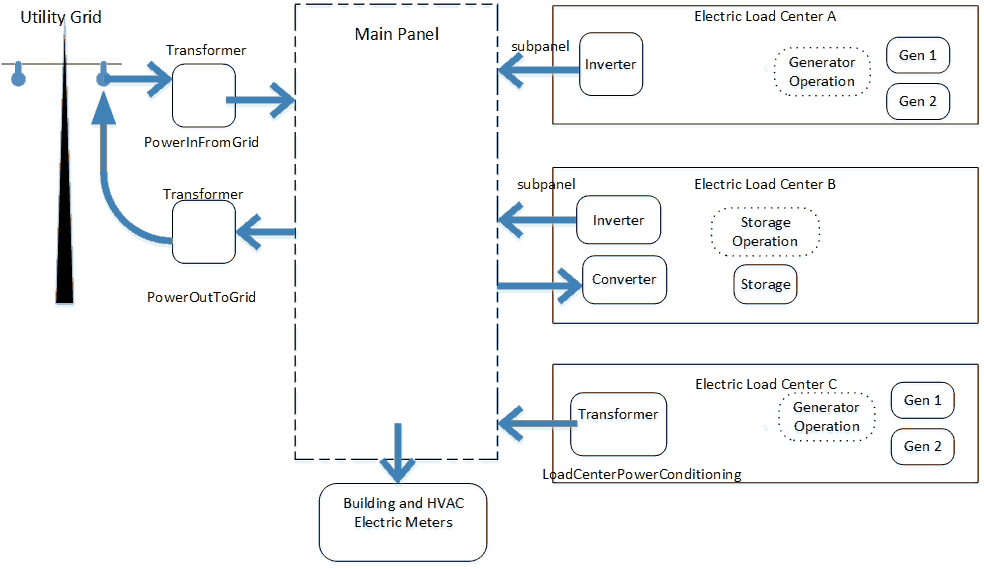
\includegraphics{media/ElectPowerServiceOverview.png}
\caption{PowerServiceOverview}
\end{figure}

\subsection{ElectricLoadCenter:Transformer}\label{electricloadcentertransformer}

This object is used to model the energy losses of transformers when they are used to transfer electricity from the grid to a building (as distribution transformers) or transfer electricity from onsite generators to the grid. Distribution transformers reduce the voltage on utility distribution lines (34.5 kV or less) to a lower secondary voltage (600 V or less) suitable for customer equipment. According to the medium used for cooling and insulation, distribution transformers can be classified into liquid-immersed and dry type transformers. According to the input voltages, distribution transformers can be classified into medium-voltage (between 600 V and 34.5kV) and low-voltage transformer (less than 600 V). The transformers used to output the surplus electricity from onsite generators to the grid usually match the cogeneration voltage to the grid. This object can be used for all types of distribution transformers and the transformers used to output electricity from onsite generators to the grid, but the model defaults applies to the low-voltage dry type transformers because they are the most common type found in commercial and industrial facilities.

Energy losses in transformers consist of the no load (core) loss and the load (winding) loss. The no load loss comes primarily from the switching of the magnetic fields in the core material. It is roughly constant and exists continuously in the core material as long as the transformer is energized. The load loss comes from the electrical resistance in the windings when there is a load on the transformer. The load loss is proportional to the load squared with a small temperature correction. The energy losses at a given load depend on the transformer's performance. This object provides the user two alternative ways to indicate the transformer's performance. First, the user can provide the no load loss and load loss at rated conditions. Second, the user can provide the nameplate efficiency and the corresponding reference conditions. The detailed algorithms to calculate the energy losses are described in the Engineering Reference.

The user needs to specify which loads are connected to the transformer. This is achieved in different manners depending on the transformer usage. For a distribution transformer, the user needs to provide a number of electric meters wired to that transformer. The input object can currently accommodate up to ten meters, but it is extensible by modifying the Energy+.idd entry. For a transformer used to output electricity from onsite generators to the grid, the user needs to indicate the transformer name in the served electric load center.

\subsubsection{Inputs}\label{inputs-014}

\paragraph{Field: Availability Schedule Name}\label{field-availability-schedule-name-005}

This alpha field contains the schedule name (ref. Schedule objects) that contains information on the availability of the transformer. A schedule value greater than 0 (usually 1 is used) indicates that the transformer is available to convert AC power from one voltage to another. A value less than or equal to 0 (usually 0 is used) denotes that the transformer is not available. If this field is blank, the schedule has values of 1 for all time periods.

\paragraph{Field: Transformer Usage}\label{field-transformer-usage}

This field indicates one of the three supported transformer application types: PowerInFromGrid, PowerOutToGrid, and LoadCenterPowerConditioning. A PowerInFromGrid type of transformer is used to step down voltage from the electricity grid to the building. The transformer with this type of use is somewhat free standing and does not need to be referenced in any \hyperref[electricloadcenterdistribution]{ElectricLoadCenter:Distribution} object. There should be only one PowerInFromGrid transformer in the model. A PowerOutToGrid type of transformer is used to match voltage from the building to the electricity grid. This conditions power exported out of the facility and feed back into the grid. This type of transformer will only be needed if the building ever exports power and the building and grid connection have different voltages. There should be only one PowerOutToGrid transformer in the model and it will serve all the surplus electricity produced by electric load center(s). A LoadCenterPowerConditioning type of transformer is used to match voltage between an electic load center (subpanel) and the facility's main panel. Each electric load center can have its own transformer to condition power fed into the main panel. For electric load centers that also draw power from the main panel, to charge storage, the transformer is assumed to operate in both directions (at the same performance). This type of transformer should be named in an \hyperref[electricloadcenterdistribution]{ElectricLoadCenter:Distribution} object.

\paragraph{Field: Zone Name}\label{field-zone-name-005}

This field contains the name of the thermal zone where the transformer is located. Entering a valid name of zone here will direct EnergyPlus to include the transformer's losses as heat gains to the named thermal zone. If the transformer is not within a thermal zone, this field can be left blank and the thermal energy associated with transformer losses is removed from the building model.

\paragraph{Field: Radiative Fraction}\label{field-radiative-fraction}

This field contains the fraction of transformer's losses that enter the zone as long-wave thermal radiation. This numeric filed should have a value between 0.0 and 1.0. The balance of the losses is convective. This field is not used if the previous field for zone name is left blank.

\paragraph{Field: Rated Capacity}\label{field-rated-capacity}

This field defines the rated capacity of the transformer in VA.

\paragraph{Field: Phase}\label{field-phase}

This field indicates whether the transformer is a single phase or three phase type. The two alternative values are 1 or 3. The default is 3. This field is currently not used in the model.

\paragraph{Field: Conductor Material}\label{field-conductor-material}

This field specifies the winding material used by the transformer. There are two options: Copper and Aluminum. The choice will determine the thermal coefficient of resistance used to calculate the temperature correction factor for the transformer load losses. The default is Aluminum.

\paragraph{Field: Full Load Temperature Rise}\label{field-full-load-temperature-rise}

This numeric field defines the temperature rise of the windings above the ambient temperature, when the transformer is loaded at its nameplate rating. For liquid-immersed distribution transformers, the full load temperature rise usually takes the value of \SI{65}{\celsius}. For dry-type transformers, the temperature rise usually takes three optional values: 80, 115 and \SI{150}{\celsius}. This field accepts any value between the minimum (\SI{50}{\celsius}) and the maximum (\SI{180}{\celsius}). The default is \SI{150}{\celsius}.

\paragraph{Field: Fraction of Eddy Current Losses}\label{field-fraction-of-eddy-current-losses}

This field defines the fraction of load losses resulting from the eddy currents. Transformer's load losses comprise two parts: the ohmic loss due to the current flowing in the resistance of the windings and the eddy and stray losses due to the eddy currents. This field indicates the fraction of the load losses due to the eddy currents. This numeric field should have a value between 0.0 and 1.0. The default is 0.1.

\paragraph{Field: Performance Input Method}\label{field-performance-input-method-000}

This alpha field contains the method by which the user will specify the transformer performance: RatedLosses or NominalEfficiency. If this field is left blank in the input data file, the default input method is assumed to be RatedLosses. If the method NominalEfficiency is selected, the user must enter the fields for the nameplate efficiency and the corresponding reference conditions as described below. If the method RatedLosses is selected, then the fields for rated no load loss and load loss must be entered as described below.

\paragraph{Field: Rated No Load Loss}\label{field-rated-no-load-loss}

This field defines the no load loss (W) at rated load and conditions. The no load loss is roughly constant and exists whenever the transformer is energized. The no load loss is also called the core loss. This field is used only if the field of Performance Input Method is specified as RatedLosses.

\paragraph{Field: Rated Load Loss}\label{field-rated-load-loss}

This field defines the load loss (W) at rated load and conditions. The load loss varies with the square of the load being served by the transformer. The load loss is also called the winding loss because the load loss occurs in the primary and secondary windings around the core. This field is used only if the field of Performance Input Method is specified as RatedLosses.

\paragraph{Field: Nameplate Efficiency}\label{field-nameplate-efficiency}

This field contains the value for transformer efficiency at a given per unit load and specified reference temperature. This field is used only if the field of Performance Input Method is specified as NominalEfficiency. The default is 0.98.

\paragraph{Field: Per Unit Load for Nameplate Efficiency}\label{field-per-unit-load-for-nameplate-efficiency}

This field defines the percentage of the rated capacity at which the nameplate efficiency is measured. According to the NEMA (National Electrical Manufactures Association) Standard TP-1, the per unit load takes the value of 0.35 for dry-type distribution transformers and it takes the value of 0.50 for liquid-filled distribution transformers. The default is 0.35.

\paragraph{Field: Reference Temperature for Nameplate Efficiency}\label{field-reference-temperature-for-nameplate-efficiency}

This field defines the conductor temperature at which the nameplate efficiency is measured. This field is used only if the field of Performance Input Method is specified as NominalEfficiency . According to the NEMA Standard TP-1, the reference temperature takes the value of \SI{75}{\celsius} for dry-type distribution transformers and it takes the value of \SI{55}{\celsius} for liquid-filled distribution transformers. The default is \SI{75}{\celsius}.

\paragraph{Field: Per Unit Load for Maximum Efficiency}\label{field-per-unit-load-for-maximum-efficiency}

This field defines the percentage of the rated capacity at which the maximum efficiency is obtained. This field is used only if the field of Performance Input Method is specified as NominalEfficiency . A blank field indicates that it takes the same value as the per unit load for nameplate efficiency.

\paragraph{Field: Consider Transformer Loss for Utility Cost}\label{field-consider-transformer-loss-for-utility-cost}

This field indicates whether the transformer losses are considered to calculate utility cost. This field applies to a PowerInFromGrid type of transformer. In some cases, the transformer losses are required but they are not part of the energy consumption for utility cost calculation. For example, the transformer is owned by the utility company but it locates in the building. In this case, it might be desired to model transformer energy losses for HVAC operation but the energy losses will not be accounted for utility cost.

\paragraph{Field: Electric Meter 1-10 Name}\label{field-electric-meter-1-10-name}

A transformer may serve different loads such as plug loads, some lighting loads, and some HVAC equipment loads. These fields apply to a PowerInFromGrid type of transformer. The user needs to specify which loads are connected to the transformer. For example the HVAC and Plant equipment might use a higher voltage than the building and only the building loads need power conditioning. This is achieved by providing a list of electric meters wired to the transformer. The input object can currently accommodate up to ten meters, but it is extensible by modifying the Energy+.idd entry. Any valid electric meter name can be used here to wire to the transformer loads. Many different meters are automatically generated by the program and will depend on the objects used throughout the input file. The typical process of determining the exact name to enter in this field involves doing an initial run of EnergyPlus and then examining the *.mdd file which will list the meters and their resulting names. A custom meter is also supported. The meter must have electricity as its resource type.

An example input of the ElectricLoadCenter:Transformer input is:

\begin{lstlisting}

ElectricLoadCenter:Transformer,
  Transformer 1,                       !-Name
  Always On,                           !- Availability Schedule Name
  PowerInFromGrid,                     !- Transformer Usage
  ,                                    !- Zone Name
  ,                                    !-Radiative Fraction
  15000,                               !- Nameplate Rating {VA}
  3,                                   !- Phase
  Aluminum,                            !- Conductor Material
  150,                                 !- Full Load Temperature Rise { &deg;C}
  0.1,                                 !- Fraction of Eddy Current Losses
  NominalEfficiency,                   !- Performance Input Method
  ,                                    !- Rated No Load Loss {W}
  ,                                    !- Rated Load Loss {W}
  0.985,                               !- Nameplate Efficiency
  0.35,                                !- Per Unit Load for Nameplate Efficiency
  75,                                  !- Reference Temperature for Nameplate Efficiency { &deg;C}
  ,                                    !- Per Unit Load for Maximum Efficiency
  Yes,                                 !- Consider Transformer Loss for Utility Cost
  Electricity:Building;                !- Meter 1 Name


  Schedule:Compact,
  Always On,                             !- Name
  Fraction,                               !- ScheduleType
  Through: 12/31,                   !- Field #1
  For: AllDays,                       !- Field #2
  Until: 24:00,                       !- Field #3
  1.0;                                         !- Field #4
\end{lstlisting}

\subsubsection{Outputs}\label{outputs-010}

\begin{itemize}
\item
  HVAC,Average,Transformer Efficiency{[]}
\item
  HVAC,Average,Transformer Output Electricity Rate {[}W{]}
\item
  HVAC,Sum,Transformer Output Elecric Energy {[}J{]}
\item
  HVAC,Average,Transformer Input Electricity Rate {[}W{]}
\item
  HVAC,Sum,Transformer Input Electricity Energy {[}J{]}
\item
  HVAC,Average,Transformer No Load Loss Rate {[}W{]}
\item
  HVAC,Sum,Transformer No Load Loss Energy {[}J{]}
\item
  HVAC,Average,Transformer Load Loss Rate {[}W{]}
\item
  HVAC,Sum,Transformer Load Loss Energy {[}J{]}
\item
  HVAC,Average,Transformer Thermal Loss Rate {[}W{]}
\item
  HVAC,Sum,Transformer Thermal Loss Energy {[}J{]}
\item
  HVAC,Sum,Transformer Distribution Electric Loss Energy {[}J{]}
\item
  HVAC,Sum,Transformer Cogeneration Electric Loss Energy {[}J{]}
\end{itemize}

\paragraph{Transformer Efficiency}\label{transformer-efficiency}

This output field is the efficiency at which the distribution transformer changes alternating current from the higher primary voltage to a lower secondary voltage. The efficiency is calculated for each HVAC system timestep being simulated, and the results are averaged for the timestep being reported.

\paragraph{Transformer Output Electricity Rate {[}W{]}}\label{transformer-output-electric-power-w}

\paragraph{Transformer Output Elecric Energy {[}J{]}}\label{transformer-output-elecric-energy-j}

These outputs are the total electricity power or energy provided by the transformer. They are equal to the metered loads which are wired to the transformer. These values are calculated for each HVAC system timestep being simulated, and the results are averaged (for power) or summed (for energy) for the timestep being reported.

\paragraph{Transformer Input Electricity Rate {[}W{]}}\label{transformer-input-electric-power-w}

\paragraph{Transformer Input Electricity Energy {[}J{]}}\label{transformer-input-electric-energy-j}

These outputs are the total electricity power or energy fed into the transformer. These values are calculated for each HVAC system timestep being simulated, and the results are averaged (for power) or summed (for energy) for the timestep being reported.

\paragraph{Transformer No Load Loss Rate {[}W{]}}\label{transformer-no-load-loss-rate-w}

\paragraph{Transformer No Load Loss Energy {[}J{]}}\label{transformer-no-load-loss-energy-j}

These outputs are the no load loss occurred in the transformer. These values are calculated for each HVAC system timestep being simulated, and the results are averaged (for rate) or summed (for energy) for the timestep being reported.

\paragraph{Transformer Load Loss Rate {[}W{]}}\label{transformer-load-loss-rate-w}

\paragraph{Transformer Load Loss Energy {[}J{]}}\label{transformer-load-loss-energy-j}

These outputs are the load loss occurred in the transformer. These values are calculated for each HVAC system timestep being simulated, and the results are averaged (for rate) or summed (for energy) for the timestep being reported.

\paragraph{Transformer Thermal Loss Rate {[}W{]}}\label{transformer-thermal-loss-rate-w}

\paragraph{Transformer Thermal Loss Energy {[}J{]}}\label{transformer-thermal-loss-energy-j}

These outputs are the total energy losses occurred in the transformer. They are equal to the sum of the no load loss and the load loss. These values are calculated for each HVAC system timestep being simulated, and the results are averaged (for rate) or summed (for energy) for the timestep being reported.

\paragraph{Transformer Distribution Electric Loss Energy {[}J{]}}\label{transformer-distribution-electric-loss-energy-j}

This output is the total energy losses occurred in the transformer when it is used for input power from grid to building. It is set as zero if the transformer is used to transfer energy from onsite power generators to the electricity grid. This output is also added to a meter with ResourceType = Electricity, GroupKey = System.

\paragraph{Transformer Cogeneration Electric Loss Energy {[}J{]}}\label{transformer-cogeneration-electric-loss-energy-j}

This output is the total energy losses occurred in the transformer when it is used for input onsite cogeneration to the grid. It is set as zero if the transformer is used to transfer the electricity grid to building. This output is also added to a meter with ResourceType = ElectricityProduced, EndUseKey = Cogeneration, GroupKey = System.

\subsection{ElectricLoadCenter:Distribution}\label{electricloadcenterdistribution}

ElectricLoadCenter:Distribution objects are used to include on-site electricity generators and or storage in a simulation. The electric load center dispatches both generators and storage according to operation schemes and tracks and reports the amount of electricity generated and purchased. When using on-site generators, the program provides various reports for the electricity used, generated on site, stored, exported etc. There are two separate operation schemes, one for generators and a second for storage, and they can be different. The generator operation is managed before the storage operation. Facility electrical demand tracking is done by the internal or custom meters used by EnergyPlus for reporting. The thermal demand tracking uses internal load calculations from the plant simulation. The dispatching of different generators is based on expectations based on their nominal/rated electric power output. If the current conditions are such that the generator model determines that generation was higher or lower, then the results of the dispatch may differ from expectations.

Multiple different ElectricLoadCenter:Distribution objects can be included in an input file. A great deal of flexibility is available by mixing different load centers and operating schemes. If multiple load centers are used, the supervisory control will dispatch generators sequentially across the load centers. Therefore, the order of these input objects in the IDF file becomes important with the generators associated with first load center in the file being the first to be managed. A certain amount of caution is needed to avoid conflicting operating schemes.

\subsubsection{Inputs}\label{inputs-1-012}

\paragraph{Field: Name}\label{field-name-013}

This alpha field contains the identifying name for the electric load center.

\paragraph{Field: Generator List Name}\label{field-generator-list-name}

This alpha field contains the identifying name for the list of generators in the set defined in an \hyperref[electricloadcentergenerators]{ElectricLoadCenter:Generators} object. All the generators connected to this load center need to be of the same type in terms of all AC or all DC. Currently the only DC generators are photovoltaic panels, the others are all AC. A facility with both AC and DC generators will need to use seperate ElectricLoadCenter:Distribution objects. The generator list named here can only be associated with one load center. This field can be left blank if there are no generators.

\paragraph{Field: Generator Operation Scheme Type}\label{field-generator-operation-scheme-type}

This alpha field specifies the type of operating scheme for the generator set. The available operating schemes are Baseload, DemandLimit, TrackElectrical, TrackSchedule, TrackMeter, FollowThermal, and FollowThermalLimitElectrical. The Baseload scheme operates the generators at their rated (requested) electric power output when the generator is scheduled ON (ref. \hyperref[electricloadcentergenerators]{ElectricLoadCenter:Generators}). The Baseload scheme requests all generators scheduled ON (available) to operate, even if the amount of electric power generated exceeds the total facility electric power demand. The DemandLimit scheme limits the amount of purchased electrical from the utility to the amount specified in the input object. The DemandLimit scheme tries to have the generators meet all of the demand above the purchased electric limit set by the user in the next field. The TrackElectrical scheme tries to have the generators meet all of the electrical demand for the building. The TrackSchedule scheme tries to have the generators meet all of the electrical demand determined in a user-defined schedule. The TrackMeter scheme tries to have the generators meet all the electrical demand from a meter, which could also be a user-defined custom meter.

The DemandLimit, TrackElectrical, TrackSchedule, and TrackMeter schemes will sequentially load the available generators. All demand not met by available generator capacity (or storage) will be met by purchased electrical. Therefore, if DemandLimit, TrackElectrical, TrackSchedule, or TrackMeter is utilized and the available generators are not enough to meet demand, then purchased electrical will offset the difference. If a generator is needed in the simulation for a small load and it is less than the minimum part load ratio the generator will operate at the minimum part load ratio and the excess will either reduce demand or the excess energy will be available for returning to the electric grid.

The FollowThermal and FollowThermalLimitElectrical schemes are for heat following cogeneration and run the generators to meet the thermal demand. The FollowThermal schemes allow excess electrical generation to be exported to the grid, while the FollowThermalLimitElectrical scheme restricts generator output to a maximum of the building's current electrical demand (so that no electricity is exported). The thermal demand is determined from the plant modeling and depends on the flow requested by other components on the demand side of the plant loop, the loop temperatures, and the loop temperature set point. The electric load center converts the thermal load to an electrical load using a nominal ratio of the thermal to electrical power production for each generator. For these schemes, the generator needs to be connected to the supply side of a plant loop and components that request hot water need to be on the demand side of the plant loop. This is different than the usual configuration for electrical following schemes where the generator is put on the demand side and request flow for the purposes of cooling the generator. Therefore a switch from one of the electrical-based operating schemes to one of the thermal-based operating schemes requires a substantial change in plant topology.

If the load center includes electrical storage, then the choice of generator operating schemes will also affect how storage is managed. The generator operation scheme and dispatch is modeled before the storage operation scheme so that the current generator production is available for use with the storage operation scheme.

\paragraph{Field: Demand Limit Scheme Purchased Electric Demand Limit}\label{field-demand-limit-scheme-purchased-electric-demand-limit}

This numerical field is the user input for the demand limit above which the generators will try and meet the entire electrical load on the building minus the photovoltaic array if available.

\paragraph{Field: Track Schedule Name Scheme Schedule Name}\label{field-track-schedule-name-scheme-schedule-name}

This alpha field is the user input for the name of a schedule defined elsewhere in the input file that contains values for the demand loads placed on the generator(s). The schedule values should be in Watts.

\paragraph{Field: Track Meter Scheme Meter Name}\label{field-track-meter-scheme-meter-name}

This alpha field is the user input for the name of a meter. Any valid meter name can be used here to control the loads that the generator(s) will try to meet. Many different meters are automatically generated by the program and will depend on the objects used throughout the input file. The typical process of determining the exact name to enter in this field involves doing an initial run of EnergyPlus and then examining the *.rdd file which will list the meters and their resulting names. The *.mtd file will also be useful to understand what exactly is included in a meter. The user can also use the Output:CustomMeter objects to redefine meter names and to control what electrical loads are included on them in a flexible manner.

\paragraph{Field: Electrical Buss Type}\label{field-electrical-buss-type}

This alpha field is used to describe how the electric load center is configured with respect to any power conditioning and/or storage equipment. There are five configurations available for load centers that are selected using one of these keywords: AlternatingCurrent, AlternatingCurrentWithStorage, DirectCurrentWithInverter, DirectCurrentWithInverterDCStorage, or DirectCurrentWithInverterACStorage. This input informs the program which of the five pre-configured arrangements is to be used for this load center. The following diagrams show the kinds of devices and how they are arranged for each of the buss types.

\begin{itemize}
\tightlist
\item
  AlternatingCurrent. This type of load center is for adding one or more on-site generators that produce AC power. If the voltage does not match a transformer can be included but is not needed. AlternatingCurrent is the default.
\end{itemize}

\begin{figure}[htbp]
\centering
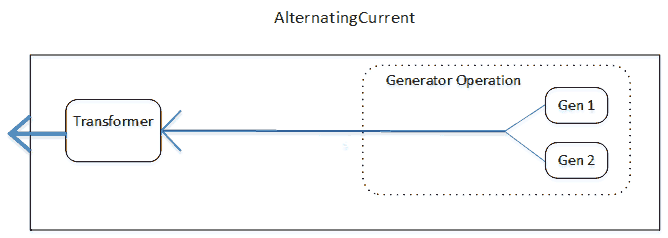
\includegraphics{media/ACBussDiagram.png}
\caption{LoadCenterBussType}
\end{figure}

\begin{itemize}
\tightlist
\item
  AlternatingCurrentWithStorage. This type of load center is for adding one or more on-site generators that produce AC power and one on-site electric storage device that uses AC power. The connection between the load center and the main building panel is bidirectional so that storage can be charged by drawing from the grid. Transformer is optional.
\end{itemize}

\begin{figure}[htbp]
\centering
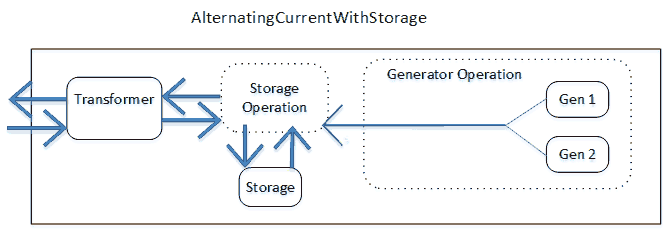
\includegraphics{media/ACStorageBussDiagram.png}
\caption{LoadCenterBussType}
\end{figure}

\begin{itemize}
\tightlist
\item
  DirectCurrentWithInverter. This type of load center is for adding one or more on-site generators that produce DC power, typically photovoltaic panels. An inverter is needed to convert generated power from DC to AC. Transformer is optional.
\end{itemize}

\begin{figure}[htbp]
\centering
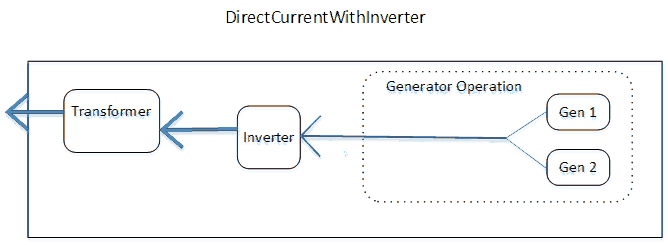
\includegraphics{media/DCInverterBussDiagram.png}
\caption{LoadCenterBussType}
\end{figure}

\begin{itemize}
\tightlist
\item
  DirectCurrentWithInverterDCStorage. This type of load center is for adding one or more on-site generatros the produce DC power and one on-site storage device that uses DC power. An inverter is needed to convert power from DC to AC and is located between the storage and where the subpanel feeds into the main panel. The connection between the load center and the main building panel is bidirectional so that storage can be charged by drawing from the grid. An AC to DC converter is needed if the storage operation scheme is such that the control might draw power from the main facility panel into the load center in order to charge storage. Transformer is optional.
\end{itemize}

\begin{figure}[htbp]
\centering
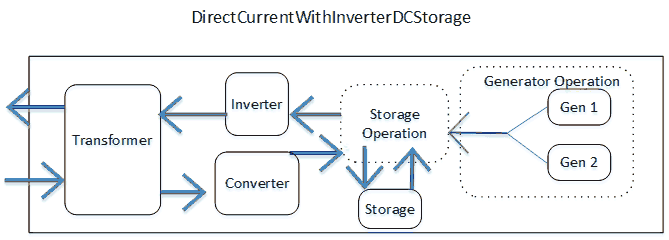
\includegraphics{media/DCInverterWithDCStorageBussDiagram.png}
\caption{LoadCenterBussType}
\end{figure}

\begin{itemize}
\tightlist
\item
  DirectCurrentWithInverterACStorage. This type of load center is for adding one or more on-site generatros the produce DC power and one on-site storage device that uses AC power. The connection between the load center and the main building panel is bidirectional so that storage can be charged by drawing from the grid. The inverter is located between the generators and the storage device. Transformer is optional.
\end{itemize}

\begin{figure}[htbp]
\centering
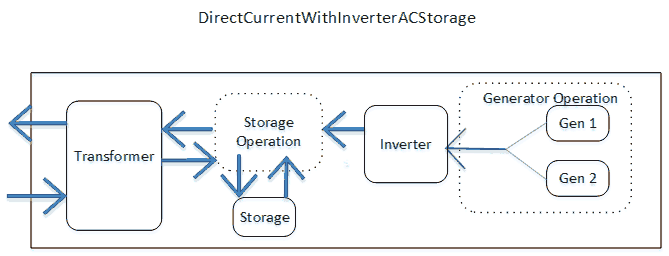
\includegraphics{media/DCInverterWithACStorageBussDiagram.png}
\caption{LoadCenterBussType}
\end{figure}

\paragraph{Field: Inverter Object Name}\label{field-inverter-object-name}

This field is used to identify the inverter connected to this load center (if any). This field is only used if the Electrical Buss Type is set to DirectCurrentWithInverter, DirectCurrentWithInverterDCStorage, or DirectCurrentWithInverterACStorage and should contain the user-defined name of an inverter object. There are three types of inverter models available -see \hyperref[electricloadcenterinvertersimple]{ElectricLoadCenter:Inverter:Simple}, \hyperref[electricloadcenterinverterlookuptable]{ElectricLoadCenter:Inverter:LookUpTable}, \hyperref[electricloadcenterinverterfunctionofpower]{ElectricLoadCenter:Inverter:FunctionOfPower}, or \hyperref[electricloadcenterinverterpvwatts]{ElectricLoadCenter:Inverter:PVWatts}. Enter the name of one of these types of inverter objects defined elsewhere in the input file.

\paragraph{Field: Electrical Storage Object Name}\label{field-electrical-storage-object-name}

This field is used to identify the electrical storage connected to this load center (if any). This field is only used if the Electrical Buss Type is set to AlternatingCurrentWithStorage, DirectCurrentWithInverterDCStorage or DirectCurrentWithInverterACStorage. Enter the name of an ElectricLoadCenter:Storage:* object defined elsewhere in the input file.

\paragraph{Field: Transformer Object Name}\label{field-transformer-object-name}

This field is used to identify the transformer connected to this load center (if any). This field can be used for any electrical buss types. Enter the name of an \hyperref[electricloadcentertransformer]{ElectricLoadCenter:Transformer} object defined elsewhere in the input file. The transformer should have use type set to LoadCenterPowerConditioning.

\paragraph{Field: Storage Operation Scheme}\label{field-storage-operation-scheme}

This field is used to select the operation scheme used to govern how storage charge and discharge is controlled. There are four options: TrackFacilityElectricDemandStoreExcessOnSite, TrackMeterDemandStoreExcessOnSite, TrackChargeDischargeSchedules, or FacilityDemandLeveling.

TrackFacilityElectricDemandStoreExcessOnSite indicates that storage control will follow the facility power demand (meter Facility:Electricity) while accounting for any on-site generation. Only excess on site generation gets stored. This is the legacy control behavior before version 8.5 and is the default.

TrackMeterDemandStoreExcessOnSite indicates that storage discharge control will follow an electric meter named in the field called Storage Control Track Meter Name. This scheme is similar TrackFacilityElectricDemandStoreExcessOnSite except that instead of the main facility electric meter, the control is based off of a user-selected meter.

TrackChargeDischargeSchedules indicates that control will follow the charging and discharging power and schedules defined in the fields called Maximum Storage Charge Grid Supply Power, Storage Charge Grid Supply Power Fraction Schedule Name, Design Storage Discharge Grid Export Power, and Storage Discharge Grid Export Fraction Schedule Name.

FacilityDemandLeveling indicates that storage control will attempt to control the facility's power demand drawn from the utility service to a prescribed level. The target utility demand is entered in the fields called Storage Control Utility Demand Limit and Storage Control Utility Demand Limit Fraction Schedule Name. This scheme first accounts for any on-site generation and during times of high use will discharge storage to reduce facility grid demand to meet the target level and during times of low use will charge storage from the grid to increase facility grid demand to meet the target level. This scheme allows controlling the load factor as long as the storage capacity and rates are not limiting what is possible. Negative schedule values can be used so that a negative demand target is exporting power out to the grid.

\paragraph{Field: Storage Control Track Meter Name}\label{field-storage-control-track-meter-name}

This field is the name of a meter to use when a custom meter is to be used. This is required when Storage Operation Scheme is set to TrackMeterDemandStoreExcessOnSite.

\paragraph{Field: Storage Converter Object Name}\label{field-storage-converter-object-name}

This field is the name of an \hyperref[electricloadcenterstorageconverter]{ElectricLoadCenter:Storage:Converter} object defined elsewhere in the input file that describes the performance when converting AC to DC when charging DC storage from grid supply. This field is required when using DC storage (buss type DirectCurrentWithInverterDCStorage) with grid supplied charging power (Storage Operation Scheme is set to TrackChargeDischargeSchedules or FacilityDemandLeveling.) Although some inverter devices are bidirectional a separate converter object is needed to describe AC to DC performance.

\paragraph{Field: Maximum Storage State of Charge Fraction}\label{field-maximum-storage-state-of-charge-fraction}

This numeric field specifies the fraction of storage capacity used as an upper limit for controlling charging. Charging will be constrained so that charging will stop the once this limit is reached. This fraction is the state of charge of the storage device where 1.0 is completely full and 0.0 is completely empty. This allows supervisory control over charging to model behavior intended to protect the battery from damage. The legacy behavior prior to version 8.5 was to charge to full capacity and therefore the default is 1.0.

\paragraph{Field: Minimum Storage State of Charge Fraction}\label{field-minimum-storage-state-of-charge-fraction}

This numeric field specifies the fraction of storage capacity used as lower limit for controlling discharging. Discharging will be constrained so that discharging will stop once this limit is reached. This fraction is the state of charge of the storage device where 1.0 is completely full and 0.0 is completely empty. This allows supervisory control over discharging to model behavior intended to protect the battery from damage. The legacy behavior prior to version 8.5 was to discharge to empty and therefore the default is 0.0.

\paragraph{Field: Design Storage Control Charge Power}\label{field-design-storage-control-charge-power}

This field is the design maximum rate that electric power can be charged into storage, in Watts. This field is used as an upper limit for most storage control operation schemes. However for TrackChargeDischargeSchedules, this is the design value for how much power to use when charging and it is multipled by the power fraction schedule in the next field. Required field when using Storage Operation Schemes set to FacilityDemandLeveling or TrackChargeDischargeSchedules.

\paragraph{Field: Storage Charge Power Fraction Schedule Name}\label{field-storage-charge-power-fraction-schedule-name}

This field contains the name of a schedule that controls the timing and magnitude of charging storage. This is a required field if Storage Operation Scheme is set to TrackChargeDischargeSchedules. Schedule values should be fractions from 0.0 to 1.0, inclusive. This schedule will need to be coordinated with the discharging schedule named below.

\paragraph{Field: Design Storage Control Discharge Power}\label{field-design-storage-control-discharge-power}

This field is the design maximum rate that electric power can be discharged from storage. This field is used as an upper limit for most storage control operation schemes. However for TrackChargeDischargeSchedules, this is the design value for how much power to draw when discharging and it is multiplied by the power fraction schedule in the next field. Required field when using Storage Operation Schemes set to FacilityDemandLeveling or TrackChargeDischargeSchedules.

\paragraph{Field: Storage Discharge Power Fraction Schedule Name}\label{field-storage-discharge-power-fraction-schedule-name}

This field contains the name of a schedule that controls the timing and magnitude of discharging storage. Required field if Storage Operation Scheme is set to TrackChargeDischargeSchedules. Schedule values should be fractions from 0.0 to 1.0, inclusive. This schedule will need to be coordinated with the charging schedule named above.

\paragraph{Field: Storage Control Utility Demand Target}\label{field-storage-control-utility-demand-target}

This field contains the design demand target in Watts. This field is used when the storage operation scheme is set to FacilityDemandLeveling. This becomes the target utility service demand power for discharge control. This design value is multiplied by the fraction schedule named in the next field. This is more than an upper limit, it is also going to call for extra electric power to raise demand up to the target and put the extra power into on-site storage. This field is required for FacilityDemandLimit storage operation scheme.

\paragraph{Field: Storage Control Utility Demand Target Fraction Schedule Name}\label{field-storage-control-utility-demand-target-fraction-schedule-name}

This field is the name of schedule that modifies the utility demand power target over time. Schedule values should be fractions from -1.0 to 1.0, inclusive. Negative values indicate export to grid. This field is required if Storage Operation Scheme is set to FacilityDemandLeveling.

Examples of this object are:

\begin{lstlisting}

ElectricLoadCenter:Distribution,
  SOFC Electric Load Center,      !- Name
  Micro-Generators,               !- Generator List Name
  Baseload,                       !- Generator Operation Scheme Type
  0.0,                            !- Demand Limit Scheme Purchased Electric Demand Limit {W}
  ,                               !- Track Schedule Name Scheme Schedule Name
  ,                               !- Track Meter Scheme Meter Name
  AlternatingCurrent,             !- Electrical Buss Type
  ,                               !- Inverter Object Name
  ;                               !- Electrical Storage Object Name


  ElectricLoadCenter:Distribution,
  Electric Load Center,       !- Name
  Backup Generators,             !- Generator List Name
  DemandLimit,                         !- Generator Operation Scheme Type
  10000.0,                                 !- Demand Limit Scheme Purchased Electric Demand Limit {W}
  ,                                               !- Track Schedule Name Scheme Schedule Name
  ,                                               !- Track Meter Scheme Meter Name
  AlternatingCurrent,           !- Electrical Buss Type
  ,                                               !- Inverter Object Name
  ;                                               !- Electrical Storage Object Name
\end{lstlisting}

\subsubsection{Outputs}\label{outputs-1-008}

There are three levels of results reporting related to electric load centers and generators. The top level of reporting provides results across the whole building and all the different electric load centers and generators. The second level of reporting provides results for individual load centers. The third level is for each type of generator (see individual generator descriptions). This section discusses the first two levels.

Even if no ElectricLoadCenter:Distribution object is included, the following whole-building summary output variables are also available for all simulations that have any electricity consuming equipment.

\begin{itemize}
\tightlist
\item
  HVAC,Average,Facility Total Purchased Electricity Rate {[}W{]}
\item
  HVAC,Sum,Facility Total Purchased Electricity Energy {[}J{]}
\item
  HVAC,Average,Facility Total Surplus Electricity Rate {[}W{]}
\item
  HVAC,Sum,Facility Total Surplus Electricity Energy {[}J{]}
\item
  HVAC,Average,Facility Net Purchased Electricity Rate {[}W{]}
\item
  HVAC,Sum,Facility Net Purchased Electricity Energy {[}J{]}
\item
  HVAC,Average,Facility Total Building Electric Demand Power {[}W{]}
\item
  HVAC,Average,Facility Total HVAC Electric Demand Power {[}W{]}
\item
  HVAC,Average,Facility Total Electric Demand Power {[}W{]}
\item
  HVAC,Average,Facility Total Produced Electricity Rate {[}W{]}
\item
  HVAC,Sum,Facility Total Produced Electricity Energy {[}J{]}
\end{itemize}

These output variables all use a default keyword Whole Building.

\paragraph{Facility Total Purchased Electricity Rate {[}W{]}}\label{facility-total-purchased-electric-power-w}

\paragraph{Facility Total Purchased Electricity Energy {[}J{]}}\label{facility-total-purchased-electric-energy-j}

These outputs are the total of electricity purchased for the entire facility in both power and energy units. This value is always positive and indicates the amount of energy that is purchased from the utility.

\paragraph{Facility Total Surplus Electricity Rate {[}W{]}}\label{facility-total-surplus-electric-power-w}

\paragraph{Facility Total Surplus Electricity Energy {[}J{]}}\label{facility-total-surplus-electric-energy-j}

These outputs are the total excess electricity exported and sent out to the electrical grid in both power and energy units. This value is always positive and indicates the surplus electric power (from generation and/or storage discharge) exceeds the whole-building demand and electricity is being fed from the facility into the grid.

\paragraph{Facility Net Purchased Electricity Rate {[}W{]}}\label{facility-net-purchased-electric-power-w}

\paragraph{Facility Net Purchased Electricity Energy {[}J{]}}\label{facility-net-purchased-electric-energy-j}

These outputs are the net electricity purchased in both Power and Energy units. This value can be either positive or negative. Positive values are defined as electricity purchased from the utility. Negative values are defined as surplus electricity fed back into the grid.

\paragraph{Facility Total Building Electric Demand Power {[}W{]}}\label{facility-total-building-electric-demand-power-w}

This output variable includes all of the electric demand from the building (non-HVAC) portion of the simulation, which would contain lights, electrical equipment, exterior lights and equipment, etc.

\paragraph{Facility Total HVAC Electric Demand Power {[}W{]}}\label{facility-total-hvac-electric-demand-power-w}

This output variable includes all of the electric demand from the HVAC portion of the simulation, which would contain fans, electric coils, pumps, chillers, cooling towers, etc.

\paragraph{Facility Total Electric Demand Power {[}W{]}}\label{facility-total-electric-demand-power-w}

This is the total of the whole Building and HVAC electric demands.

\paragraph{Facility Total Produced Electricity Rate {[}W{]}}\label{facility-total-produced-electric-power-w}

\paragraph{Facility Total Produced Electricity Energy {[}J{]}}\label{facility-total-produced-electric-energy-j}

These outputs are the total generator and photovoltaic electricity produced on-site for the entire model, and they are in both Power and Energy units. When the electric power production system includes power conversion devices including DC to AC inverters, AC to DC converters, or transformers, the power conversion losses are included as negative values in these reports. When electrical storage is used with on-site production, the electricity put into storage is decremented from production and the electricity removed storage is added to production. This means that losses from a round trip through electrical storage decrease on-site electricity production.

Each ElectricLoadCenter also collects results from the individual generators that are connected to that load center. The keywords for these reports are the unique names of ElectricLoadCenter:Distribution objects. The output variables available at the ElectricLoadCenter level are:

\begin{itemize}
\tightlist
\item
  HVAC,Average,Electric Load Center Produced Electricity Rate {[}W{]}
\item
  HVAC,Sum,Electric Load Center Produced Electricity Energy {[}J{]}
\item
  HVAC,Average,Electric Load Center Supplied Electricity Rate {[}W{]}
\item
  HVAC,Average,Electric Load Center Drawn Electricity Rate {[}W{]}
\item
  HVAC,Average,Electric Load Center Produced Thermal Rate {[}W{]}
\item
  HVAC,Sum,Electric Load Center Produced Thermal Energy {[}J{]}
\item
  HVAC,Average,Electric Load Center Requested Electricity Rate {[}W{]}
\end{itemize}

\paragraph{Electric Load Center Produced Electricity Rate {[}W{]}}\label{electric-load-center-produced-electric-power-w}

\paragraph{Electric Load Center Produced Electricity Energy {[}J{]}}\label{electric-load-center-produced-electric-energy-j}

These outputs are the sum of electrical energy and power produced by the generators attached to a particular load center. This could be DC or AC depending on the type of buss. The power actually delivered by the load center may be adjusted by power conversion losses from an inverter or transformer or by interaction with the any electrical storage.

\paragraph{Electric Load Center Supplied Electricity Rate {[}W{]}}\label{electric-load-center-supplied-electric-power-w}

This output is the power fed from the electric load center into the main distribution panel, in Watts. This power is generated or discharged by on site equipment and has been adjusted to account for any power conversion by an inverter and/or transformer on the load center.

\paragraph{Electric Load Center Drawn Electricity Rate {[}W{]}}\label{electric-load-center-drawn-electric-power-w}

This output is the power fed from the main distribution panel into the load center, in Watts. This power draw is typically only for charging storage with power from either the grid or another load center.

\paragraph{Electric Load Center Produced Thermal Rate {[}W{]}}\label{electric-load-center-produced-thermal-rate-w}

\paragraph{Electric Load Center Produced Thermal Energy {[}J{]}}\label{electric-load-center-produced-thermal-energy-j}

These outputs are the sum of the thermal energy and power produced by the generators attached to a particular load center. The keywords for these reports are the unique names of ElectricLoadCenter:Distribution objects.

\paragraph{Electric Load Center Requested Electricity Rate {[}W{]}}\label{electric-load-center-requested-electric-power-w}

This output variable is the average electric power supply (in watts) requested of the load center by the facility's main distribution panel, for the time step being reported. This is used by the load center generator and storage operation control logic when determining how to run the generators and/or storage devices. For the baseload generator operating scheme, this output variable should equal the sum of the power supply requests for the available generators associated with this load center (ref. ElectricLoadCenter:Generators). In other cases, this output could be different from the sum of the power supply requests for the generators associated with this load center. For example, a generator might be requested to provide a certain amount of power but can only provide a fraction of the requested amount. In this case the load center will detect this shortfall and include it when calculating the power request for the next available generator. Therefore, the sum of the power supply requests for the individual generators associated with this load center (ref. ElectricLoadCenter:Generators) could be greater than the Electric Load Center Requested Electric Power output variable.

\subsection{ElectricLoadCenter:Generators}\label{electricloadcentergenerators}

The ElectricLoadCenter:Generators object is used to provide a list of the generators to include in the simulation. The list includes the names and types of all the generators along with separate availability schedules, the rated power output, and thermal-to-electrical power ratio for each. Sets of five input fields are repeated for each generator. If more than 30 generators are needed, EnergyPlus will auto-extend to suit the needs but other interfaces (such as the IDF Editor may not). The user can always modify the Energy+.idd file to accommodate the extra fields necessary, but it is likely the next release of EnergyPlus will overwrite any user modifications.

\subsubsection{Inputs}\label{inputs-2-011}

\paragraph{Field: Name}\label{field-name-1-011}

This alpha field contains the identifying name for the generators in the set.

\paragraph{FieldSet: Name, Object Type, Rated Power Output, Availability, Thermal Ratio up to 30}\label{fieldset-name-object-type-rated-power-output-availability-thermal-ratio-up-to-30}

Each generator is specified by a set of 5 input fields that contain an identifying name, a keyword that indicates the type of generator, the rated output of the generator, the availability schedule of the generator, and the thermal to electrical power production ratio.

\paragraph{Field: Generator \textless{}x\textgreater{} Name}\label{field-generator-x-name}

This alpha field contains the identifying name for the first generator in the list.

\paragraph{Field: Generator \textless{}x\textgreater{} Object Type}\label{field-generator-x-object-type}

This alpha field contains the keyword for the type of generator. The available types include:

\begin{itemize}
\item
  \hyperref[generatorinternalcombustionengine]{Generator:InternalCombustionEngine}
\item
  \hyperref[generatorcombustionturbine]{Generator:CombustionTurbine}
\item
  \hyperref[generatorphotovoltaic-000]{Generator:Photovoltaic}
\item
  \hyperref[generatorpvwatts]{Generator:PVWatts}
\item
  \hyperref[generatorfuelcell]{Generator:FuelCell}
\item
  \hyperref[generatormicrochp]{Generator:MicroCHP}
\item
  \hyperref[generatormicroturbine]{Generator:MicroTurbine}
\item
  \hyperref[generatorwindturbine]{Generator:WindTurbine}
\end{itemize}

These keywords are the names of the input objects for the type of generator.

\paragraph{Field: Generator \textless{}x\textgreater{} Rated Electric Power Output}\label{field-generator-x-rated-electric-power-output}

This numeric field contains the nominal electric power output to be requested from generator 1. It is normally equal to the rated power output of the generator in Watts. This value is used only for supervisory control and generator dispatch; the actual power output for each time step is determined by the generator models. This value affects how much a generator is loaded (i.e., requested electric power output) and can also impact the operation of an electric storage unit (e.g., LoadCenter:Storage:Simple) if one is connected to the associated load distribution center (ref. \hyperref[electricloadcenterdistribution]{ElectricLoadCenter:Distribution}). Refer to Electrical Storage in the EnergyPlus Engineering Reference for more details regarding this input field and its relationship with electric storage.

\paragraph{Field: Generator \textless{}x\textgreater{} Availability Schedule Name}\label{field-generator-x-availability-schedule-name}

This alpha field is used as an identifying field for the generator availability schedule. If not blank, this field must contain the name of a schedule defined elsewhere in the input file. A schedule value of \textless{} = 0.0 indicates the generator is not available, while a schedule value \textgreater{} 0.0 indicates that the generator is available to operate. If this field is blank, the schedule has values of 1 for all time periods.

\paragraph{Field: Generator \textless{}x\textgreater{} Rated Thermal to Electrical Power Ratio}\label{field-generator-x-rated-thermal-to-electrical-power-ratio}

This numeric field contains the ratio of the rated thermal output to the rated electric output. It is required and used if the operation scheme is set to \textbf{FollowThermal} or \textbf{FollowThermalLimitElectrical}. This nominal ratio is only used for control and dispatch decisions. This value should be generally consistent with the more detailed performance input for the individual generator component models but it is not used in those component models.

An example IDF showing how this object is used is provided below:

\begin{lstlisting}

ElectricLoadCenter:Generators,
  Backup Generators,             !- Name
  Cat Diesel,                           !- Generator 1 Name
  Generator:InternalCombustionEngine,   !- Generator 1 Object Type
  50000,                                     !- Generator 1 Rated Electric Power Output
  ON PEAK GENERATOR SCHEDULE,   !- Generator 1 Availability Schedule Name
  ,                                               !- Generator 1 Rated Thermal to Electrical Power Ratio
  Solar Turbine,                     !- Generator 2 Name
  Generator:CombustionTurbine,   !- Generator 2 Object Type
  30000,                                     !- Generator 2 Rated Electric Power Output
  OFF PEAK GENERATOR SCHEDULE,   !- Generator 2 Availability Schedule Name
  ,                                               !- Generator 2 Rated Thermal to Electrical Power Ratio
  Capstone C65,                       !- Generator 3 Name
  Generator:Microturbine,   !- Generator 3 Object Type
  65000,                                     !- Generator 3 Rated Electric Power Output
  MID PEAK GENERATOR SCHEDULE,   !- Generator 3 Availability Schedule Name
  ;                                               !- Generator 3 Rated Thermal to Electrical Power Ratio
\end{lstlisting}

\subsubsection{Outputs}\label{outputs-2-007}

A single output variable is available for each generator specified via this object as described below:

\begin{itemize}
\tightlist
\item
  HVAC,Average,Generator Requested Electricity Rate {[}W{]}
\end{itemize}

\paragraph{Generator Requested Electricity Rate {[}W{]}}\label{generator-requested-electric-power-w}

This output variable represents the average electric power supply in Watts that is being requested by the generator operation scheme from a specific generator for the time step being reported. In some instances the output value may be the Rated Electric Power Output specified for the generator in the ElectricLoadCenter:Generators object. If the generator is not available for a simulation time step (as indicated by its availability schedule), then the power supply request will be zero. The power supply request may be less than the rated electric power output if the overall electric power reduction target has already been met, partially or completely, by electric power produced by other generators. If an EnergyPlus Energy Management System is used to specify an electric power supply request for this generator, then that EMS request will be reflected in this output variable.

\subsection{ElectricLoadCenter:Inverter:Simple}\label{electricloadcenterinvertersimple}

This input object is used to model conversion from Direct Current (DC) to Alternating Current (AC) in an electric load center that contains photovoltaic modules. Such a load center has an array of photovoltaic modules that feed an inverter DC power and the inverter produces AC power. This input object is for the simplest inverter model and uses a fixed efficiency. There are two other types of inverters with more complex models described below.

\subsubsection{Inputs}\label{inputs-3-010}

\paragraph{Field: Name}\label{field-name-2-010}

This field contains a unique name for the inverter. The name entered must also be unique across all other types of inverters that may also be in the input file.

\paragraph{Field: Availability Schedule Name}\label{field-availability-schedule-name-1-003}

This field contains the name of a schedule that describes when the inverter is available. If the inverter is scheduled to not be available, by scheduling a value of 0, then it cannot produce AC power and will not consume ancillary power during standby. Any non-zero schedule value means the inverter is available to produce AC power and consume ancillary power during standby. If the Inverter is scheduled to be unavailable but it is being supplied with DC power anyway, then the energy is dissipated as heat. If this field is blank, the schedule has values of 1 for all time periods.

\paragraph{Field: Zone Name}\label{field-zone-name-1-003}

This field contains the name of the thermal zone where the inverter is located. Entering a valid name of zone here will direct EnergyPlus to include the inverter's losses as heat gains to the named thermal zone. If the inverter is not within a thermal zone, then this field can be left blank (and the thermal energy associated with inverter losses is removed from the building model).

\paragraph{Field: Radiative Fraction}\label{field-radiative-fraction-1}

This field contains the fraction of inverter thermal losses that enter the zone as long-wave thermal radiation. This should be a factor between 0.0 and 1.0. The balance of the losses is convective. This field is not used if the previous field for zone name is left blank.

\paragraph{Field: Inverter Efficiency}\label{field-inverter-efficiency}

This field contains the value for inverter efficiency. In the simple model, efficiency is a constant. This is the so-called 1-term model. Input data for different types of inverters is available at \url{http://www.gosolarcalifornia.org/equipment/inverter_tests/summaries} where the CEC Efficiency would be the value to enter here.

An example IDF showing how this object is used is provided below:

\begin{lstlisting}

ElectricLoadCenter:Inverter:Simple,
  Simple Ideal Inverter,     !- Name
  Always On,                             !- Availability Schedule Name
  ,                                               !- Zone Name
  0.0,                                         !- Radiative Fraction
  1.0;                                         !- Inverter Efficiency
\end{lstlisting}

\subsection{ElectricLoadCenter:Inverter:FunctionOfPower}\label{electricloadcenterinverterfunctionofpower}

This input object is used to model conversion from Direct Current (DC) to Alternating Current (AC) in an electric load center that contains photovoltaic modules. Such a load center has an array of photovoltaic modules that feed an inverter DC power and the inverter produces AC power. This input object is for an inverter model where efficiency is a function of normalized power.

\subsubsection{Inputs}\label{inputs-4-009}

\paragraph{Field: Name}\label{field-name-3-009}

This field contains a unique name for the inverter. The name entered must also be unique across all other types of inverters that may also be in the input file.

\paragraph{Field: Availability Schedule Name}\label{field-availability-schedule-name-2-001}

This field contains the name of a schedule that describes when the inverter is available. If the inverter is scheduled to not be available, by scheduling a value of 0, then it cannot produce AC power, nor contribute heat gains to the zone, and will not consume ancillary power during standby. Any non-zero schedule value means the inverter is available to produce AC power, contribute heat gains to the zone and consume ancillary power during standby. If this field is blank, the schedule has values of 1 for all time periods.

\paragraph{Field: Zone Name}\label{field-zone-name-2-001}

This field contains the name of the thermal zone where the inverter is located. Entering a valid name of zone here will direct EnergyPlus to include the inverter's losses as heat gains to the named thermal zone. If the inverter is not within a thermal zone, then this field can be left blank (and the thermal energy associated with inverter losses is removed from the building model).

\paragraph{Field: Radiative Fraction}\label{field-radiative-fraction-2}

This field contains the fraction of inverter thermal losses that enter the zone as long-wave thermal radiation. This should be a factor between 0.0 and 1.0. The balance of the losses is convective. This field is not used if the previous field for zone name is left blank.

\paragraph{Field: Efficiency Function of Power Curve Name}\label{field-efficiency-function-of-power-curve-name}

This field contains the name of curve representing the relationship between DC power input into the inverter and the efficiency with which that power is converted to AC. The curve can be either a \hyperref[curvelinear]{Curve:Linear}, \hyperref[curvequadratic]{Curve:Quadratic}, or \hyperref[curvecubic]{Curve:Cubic}. The curve's x value is DC power input normalized by the following field. The result of the curve should be power conversion efficiency expressed as a fraction between 0.0 and 1.0.

\paragraph{Field: Rated Maximum Continuous Input Power}\label{field-rated-maximum-continuous-input-power}

This field contains the rated power input in watts. This is value used to normalize input power for use with the curve named in the previous field. This is DC power from the PV arrays going into the inverter.

\paragraph{Field: Minimum Efficiency}\label{field-minimum-efficiency}

This field contains a minimum bound on the inverter efficiency. This value will be used as a limit on the curve's result.

\paragraph{Field: Maximum Efficiency}\label{field-maximum-efficiency}

This field contains a maximum bound on the inverter efficiency. This value will be used as a limit on the curve's result.

\paragraph{Field: Minimum Power Output}\label{field-minimum-power-output}

This field contains a lower limit on the AC power produced by the inverter. If the resulting power output would be below this level, then the inverter is assumed to not produce any power and is in standby mode. All DC power input is lost (unless it is going into storage).

\paragraph{Field: Maximum Power}\label{field-maximum-power}

This field contains an upper limit on the AC power produced by the inverter. If the resulting power output would be above this level, then the power produced is capped at this level with the rest of input power converted to losses (unless it is going into storage).

\paragraph{Field: Ancillary Power Consumed In Standby}\label{field-ancillary-power-consumed-in-standby}

This field contains the ancillary power in watts used by the inverter when not producing AC power. This is AC electricity consumed in standby mode. Standby mode occurs when the inverter is scheduled to be available but the incoming DC power is too low.

An example IDF showing how this object is used is provided below:

\begin{lstlisting}

ElectricLoadCenter:Inverter:FunctionOfPower,
  Curve Inverter,                   !- Name
  ALWAYS_ON,                             !- Availability Schedule Name
  ,                                               !- Zone Name
  0.3,                                         !- Radiative Fraction
  Inverter Curve,                   !- Efficiency Function of Power Curve Name
  15000,                                     !- Rated Maximum Continuous Input Power {W}
  0.0,                                         !- Minimum Efficiency
  1.0,                                         !- Maximum Efficiency
  200,                                         !- Minimum Power Output {W}
  20000,                                     !- Maximum Power Output {W}
  0.0;                                         !- Ancillary Power Consumed In Standby {W}
\end{lstlisting}

\subsection{ElectricLoadCenter:Inverter:LookUpTable}\label{electricloadcenterinverterlookuptable}

This input object is used to model conversion from Direct Current (DC) to Alternating Current (AC) in an electric load center that contains photovoltaic modules. Such a load center has an array of photovoltaic modules that feed an inverter DC power and the inverter produces AC power. This input object is for an inverter model where efficiency is interpolated using a look up table.

This object was designed for use with data contained in the Inverter Performance Test Summaries available at \url{http://www.gosolarcalifornia.org/equipment/inverter_tests/summaries}. All of the data needed for this object can be found there by make and model of inverter. The core of the data set is a 3x6 matrix of efficiency at different voltage and power levels. These form the look up table used in the model. Note that EnergyPlus PV models currently model only power and not the voltage and current situation. Therefore, only the nominal voltage data are used. This is the middle row of data in the Go Solar summaries.

\subsubsection{Inputs}\label{inputs-5-008}

\paragraph{Field: Name}\label{field-name-4-008}

This field contains a unique name for the inverter. The name entered must also be unique across all other types of inverters that may also be in the input file.

\paragraph{Field: Availability Schedule Name}\label{field-availability-schedule-name-3-001}

This field contains the name of a schedule that describes when the inverter is available. If the inverter is scheduled to not be available, by setting a value of 0, then it cannot produce AC power, nor contribute heat gains to the zone, and will not consume ancillary power during standby. Any non-zero schedule value means the inverter is available to produce AC power, contribute heat gains to the zone and consume ancillary power during standby. If this field is blank, the schedule has values of 1 for all time periods.

\paragraph{Field: Zone Name}\label{field-zone-name-3-000}

This field contains the name of the thermal zone where the inverter is located. Entering a valid name of zone here will direct EnergyPlus to include the inverter's losses as heat gains to the named thermal zone. If the inverter is not within a thermal zone, then this field can be left blank (and the thermal energy associated with inverter losses is removed from the building model).

\paragraph{Field: Radiative Fraction}\label{field-radiative-fraction-3}

This field contains the fraction of inverter thermal losses that enter the zone as long-wave thermal radiation. This should be a factor between 0.0 and 1.0. The balance of the losses is convective. This field is not used if the previous field for zone name is left blank.

\paragraph{Field: Rated Maximum Continuous Output Power}\label{field-rated-maximum-continuous-output-power}

This field contains the rated maximum continuous output power in watts.

\paragraph{Field: Night Tare Loss Power}\label{field-night-tare-loss-power}

This field contains the night tare loss in watts. This is modeled as ancillary power consumed during standby.

\paragraph{Field: Nominal Voltage Input}\label{field-nominal-voltage-input}

This field contains the nominal DC input voltage in volts. This is Vnom in the Go Solar test summaries.

\paragraph{Field: Efficiency at 10\% Power and Nominal Voltage}\label{field-efficiency-at-10-power-and-nominal-voltage}

This field contains the fractional efficiency at nominal voltage and 10\% power.

\paragraph{Field: Efficiency at 20\% Power and Nominal Voltage}\label{field-efficiency-at-20-power-and-nominal-voltage}

This field contains the fractional efficiency at nominal voltage and 20\% power.

\paragraph{Field: Efficiency at 30\% Power and Nominal Voltage}\label{field-efficiency-at-30-power-and-nominal-voltage}

This field contains the fractional efficiency at nominal voltage and 30\% power.

\paragraph{Field: Efficiency at 50\% Power and Nominal Voltage}\label{field-efficiency-at-50-power-and-nominal-voltage}

This field contains the fractional efficiency at nominal voltage and 50\% power.

\paragraph{Field: Efficiency at 75\% Power and Nominal Voltage}\label{field-efficiency-at-75-power-and-nominal-voltage}

This field contains the fractional efficiency at nominal voltage and 75\% power.

\paragraph{Field: Efficiency at 100\% Power and Nominal Voltage}\label{field-efficiency-at-100-power-and-nominal-voltage}

This field contains the fractional efficiency at nominal voltage and 100\% power.

An example IDF showing how this object is used is provided below:

\begin{lstlisting}

ElectricLoadCenter:Inverter:LookUpTable,
  PV Inverter,                         !- Name
  ALWAYS_ON,                             !- Availability Schedule Name
  ,                                               !- Zone Name
  0.25,                                       !- Radiative Fraction
  14000,                                     !- Rated Maximum Continuous Output Power {W}
  200.0,                                     !- Night Tare Loss Power {W}
  368,                                         !- Nominal Voltage Input {V}
  0.839,                                     !- Efficiency at 10% Power and Nominal Voltage
  0.897,                                     !- Efficiency at 20% Power and Nominal Voltage
  0.916,                                     !- Efficiency at 30% Power and Nominal Voltage
  0.931,                                     !- Efficiency at 50% Power and Nominal Voltage
  0.934,                                     !- Efficiency at 75% Power and Nominal Voltage
  0.930;                                     !- Efficiency at 100% Power and Nominal Voltage
\end{lstlisting}

\subsection{ElectricLoadCenter:Inverter:PVWatts}\label{electricloadcenterinverterpvwatts}

The ElectricLoadCenter:Inverter:PVWatts is intended to be used in an \hyperref[electricloadcenterdistribution]{ElectricLoadCenter:Distribution} with one or more \hyperref[generatorpvwatts]{Generator:PVWatts} objects. It is \textbf{not} compatible with other Generator objects, such as \hyperref[generatorphotovoltaic-000]{Generator:Photovoltaic}.

\subsubsection{Inputs}\label{inputs-electricloadcenterinverterpvwatts}

\paragraph{Field: Name}\label{field-name-electricloadcenterinverterpvwatts}

This field contains a unique name for the inverter. The name entered
must also be unique across all other types of inverters that may also be
in the input file.

\paragraph{Field: DC to AC Size ratio}\label{field-dc-to-ac-size-ratio-electricloadcenterinverterpvwatts}

The DC to AC size ratio is the ratio of the inverter's AC rated size to
the array's DC rated size. Increasing the ratio increases the system's
output over the year, but also increases the array's cost. The default
value is 1.10, which means that a 4 kW system size would be for an array
with a 4 DC kW nameplate size at standard test conditions (STC) and an
inverter with a 3.63 AC kW nameplate size.

For a system with a high DC to AC size ratio, during times when the
array's DC power output exceeds the inverter's rated DC input size, the
inverter limits the array's power output by increasing the DC operating
voltage, which moves the array's operating point down its
current-voltage (I-V) curve. PVWatts models this effect by limiting the
inverter's power output to its rated AC size.

The default value of 1.10 is reasonable for most systems. A typical
range is 1.10 to 1.25, although some large-scale systems have ratios of
as high as 1.50. The optimal value depends on the system's location,
array orientation, and module cost.

Default: 1.10

\paragraph{Field: Inverter Efficiency}\label{field-inverter-efficiency-electricloadcenterinverterpvwatts}

The inverter's nominal rated DC-to-AC conversion efficiency, defined as
the inverter's rated AC power output divided by its rated DC power
output.

Default: 0.96

\subsubsection{Outputs Description}\label{outputs-description-electricloadcenterinverterpvwatts}

\begin{itemize}
\item
  HVAC,Average,Inverter Produced AC Electricity Rate {[}W{]}
\item
  HVAC,Sum,Inverter Produced AC Electricity Energy {[}J{]}
\end{itemize}

\subsubsection{Outputs}\label{outputs-3-005}

Each inverter can report the following seven output variables.

\begin{itemize}
\tightlist
\item
  HVAC,Average,Inverter DC to AC Efficiency {[]}
\item
  HVAC,Average,Inverter DC Input Electricity Rate {[}W{]}
\item
  HVAC,Sum,Inverter DC Input Electricity Energy {[}J{]}
\item
  HVAC,Average,Inverter AC Output Electricity Rate {[}W{]}
\item
  HVAC,Sum,Inverter AC Output Electricity Energy {[}J{]}
\item
  HVAC,Average,Inverter Conversion Loss Power {[}W{]}
\item
  HVAC,Sum,Inverter Conversion Loss Energy {[}J{]}
\item
  HVAC,Sum,Inverter Conversion Loss Decrement Energy {[}J{]}
\item
  HVAC,Average,Inverter Thermal Loss Rate {[}W{]}
\item
  HVAC,Sum,Inverter Thermal Loss Energy {[}J{]}
\item
  HVAC,Average,Inverter Ancillary AC Electricity Rate {[}W{]}
\item
  HVAC,Sum,Inverter Ancillary AC Electricity Energy {[}J{]}
\end{itemize}

\paragraph{Inverter DC to AC Efficiency {[]}}\label{inverter-dc-to-ac-efficiency}

This is the efficiency with which DC power is converted to AC power by the inverter.

\paragraph{Inverter DC Input Elecric Power {[}W{]}}\label{inverter-dc-input-elecric-power-w}

\paragraph{Inverter DC Input Electricity Energy {[}J{]}}\label{inverter-dc-input-electric-energy-j}

These outputs are total electricity power or energy fed into the inverter. This is Direct Current from photovoltaics (or DC-based electrical storage) going into the inverter.

\paragraph{Inverter AC Output Electricity Rate {[}W{]}}\label{inverter-ac-output-electric-power-w}

\paragraph{Inverter AC Output Electricity Energy {[}J{]}}\label{inverter-ac-output-electric-energy-j}

These outputs are the total electricity power or energy produced by the inverter. This is Alternating Current going out of the inverter.

\paragraph{Inverter Conversion Loss Power {[}W{]}}\label{inverter-conversion-loss-power-w}

\paragraph{Inverter Conversion Loss Energy {[}J{]}}\label{inverter-conversion-loss-energy-j}

\paragraph{Inverter Conversion Loss Decrement Energy {[}J{]}}\label{inverter-conversion-loss-decrement-energy-j}

These outputs are the thermal power or energy losses in the inverter that stem from converting from DC to AC. The decrement energy is negative and is metered as ``PowerConversion'' on the ``ElectricityProduced'' resource.

\paragraph{Inverter Thermal Loss Rate {[}W{]}}\label{inverter-thermal-loss-rate-w}

\paragraph{Inverter Thermal Loss Energy {[}J{]}}\label{inverter-thermal-loss-energy-j}

These outputs are the thermal power or energy losses in the inverter that stem from converting from DC to AC plus any ancillary electric power.

\paragraph{Inverter Ancillary AC Electricity Rate {[}W{]}}\label{inverter-ancillary-ac-electric-power-w}

\paragraph{Inverter Ancillary AC Electricity Energy {[}J{]}}\label{inverter-ancillary-ac-electric-energy-j}

These outputs are the Alternating Current electricity consumed by the inverter. These are ancillary, or night tare loss, power uses by the inverter and modeled as if powered by the building's grid connection. These ancillary power draws generally occur when the inverter is not generating power but waiting in a standby mode ready to begin generating power.

\subsection{ElectricLoadCenter:Storage:Converter}\label{electricloadcenterstorageconverter}

This model is for converting AC to DC for grid-supplied charging of DC storage. The model is only for power conversion and does not consider voltage. There are two methods available for determining the efficiency with which power is converted. The efficiency is defined as the ratio of DC power output divided by AC power input. If the name of a zone is entered the power conversion losses will be added to the zone as internal heat gains. The converter is part of a single electric load center.

\subsubsection{Field: Name}\label{field-name-5-007}

This field contains a unique name for the AC to DC converter. This name will be referenced in an \hyperref[electricloadcenterdistribution]{ElectricLoadCenter:Distribution} object.

\subsubsection{Field: Availability Schedule Name}\label{field-availability-schedule-name-4-001}

This field contains the name of a schedule that describes when the power converter is available. If power conversion is not available then electric power from the grid cannot be used to charge storage. Any non-zero value means the converter is available. If this field is blank, the schedule has a value of 1 for all time periods and the converter is always available. Standby power consumption is on when converter is available and off when the converter is not available.

\subsubsection{Field: Power Conversion Efficiency Method}\label{field-power-conversion-efficiency-method}

This choice field is used to select which method is used to define the efficiency with which power is converted from AC to DC. There are two options: SimpleFixed or FunctionOfPower. - SimpleFixed indicates that power conversion efficiency is a constant with the value set in the next field. There is no need to size the converter (with a value in the field called Design Maximum Continuous Input Power) and varying levels of power do not affect the efficiency. SimpleFixed is the default. - FunctionOfPower indicates that the power conversion efficiency is a function of the level of power being converted. This method is intended to model the characteristic that converters tend to operate less efficiently when loaded well below their design size. The converter must be sized with a value in the Design Maximum Continuous Input Power and the functional relationship described in a performance curve or look-up table.

\subsubsection{Field: Simple Fixed Efficiency}\label{field-simple-fixed-efficiency}

This numeric field is used to set a constant efficiency for conversion of AC to DC at all power levels. This field is only used, and is required, when the Power Conversion Efficiency Method is set to SimpleFixed. The value must be greater than 0.0 and less than equal to 1.0. The default is 0.95.

\subsubsection{Field: Design Maximum Continuous Input Power}\label{field-design-maximum-continuous-input-power}

This numeric field describes the size of the power converter in terms of its design input power level, in Watts. This is the AC power going into the converter. This field is only used, and is required, when the Power Conversion Efficiency Method is set to FunctionOfPower. This input serves as an upper limit for the AC power input and is used to normalize power for use in the performance curve or table. The AC power being converted at any given time is divided by the value in this field.

\subsubsection{Field: Efficiency Function of Power Curve Name}\label{field-efficiency-function-of-power-curve-name-1}

This field is the name of a performance curve or table object that describes how efficiency varies as a function of normalized power. The single independent ``x'' variable input for the curve or table is the ratio of AC input power at a given time divided by design power in the previous field. The result of the curve should be the power conversion efficiency for that normalized power so that DC power output is the product of efficiency multiplied by the AC power input. Any of the single-variable performance curves or lookup table objects can be used to describe performance. This field is only used, and is required, when the Power Conversion Efficiency Method is set to FunctionOfPower.

\subsubsection{Field: Ancillary Power Consumed In Standby}\label{field-ancillary-power-consumed-in-standby-1}

This numeric field describes the ancillary power consumed by the converter when it is available but not converting power, in Watts. This field is optional and can be used with any of the efficiency methods. If this converter is really on mode of a bidirectional inverter, take care not to double count the ancillary consumption by including them in both this component and the inverter component.

\subsubsection{Field: Zone Name}\label{field-zone-name-4-000}

This field is the name of thermal zone where the converter is located. If this field is omitted then the converter is considered outdoors. The power lost during the conversion process is treated as heat gains and added the thermal zone named in this field. The split between radiation and convection can be controlled in the next input field.

\subsubsection{Field: Radiative Fraction}\label{field-zone-rad-fract}

This numeric field is the fraction of zone heat gains that are handled as infrared thermal radiation. This field is only used if a zone is named in the previous field. The portion of zone gains that are not radiative are added to the zone as convection. If a zone is named and this field left blank or omitted then all the zone heat gains will be convective.

An example IDF showing how this object is used is provided below:

\begin{lstlisting}

ElectricLoadCenter:Storage:Converter,
  Grid Charge Converter , !- Name
  ALWAYS\_ON , !- Availability Schedule Name
  SimpleFixed , !- Power Conversion Efficiency Method
  0.95 , !- Simple Fixed Efficiency
  , !- Design Maximum Continuous Input Power
  , !- Efficiency Function of Power Curve Name 20
  , !- Ancillary Power Consumed In Standby
  , !- Zone Name 0.25; !- Radiative Fraction
\end{lstlisting}

\subsection{Electric Load Center Converter Outputs}\label{electric-load-center-converter-outputs}

Each converter can report the following output variables

\begin{itemize}
\tightlist
\item
  HVAC,Average,Converter AC to DC Efficiency {[]}
\item
  HVAC,Average,Converter AC Input Electricity Rate {[}W{]}
\item
  HVAC,Sum,Converter AC Input Electricity Energy {[}J{]}
\item
  HVAC,Average,Converter DC Output Electricity Rate {[}W{]}
\item
  HVAC,Sum,Converter DC Output Electricity Energy {[}J{]}
\item
  HVAC,Average,Converter Electric Loss Power {[}W{]}
\item
  HVAC,Sum,Converter Electric Loss Energy {[}J{]}
\item
  HVAC,Sum,Converter Electric Loss Decrement Energy {[}J{]}
\item
  HVAC,Average,Converter Thermal Loss Rate {[}W{]}
\item
  HVAC,Sum,Converter Thermal Loss Energy {[}J{]}
\item
  HVAC,Average,Converter Ancillary AC Electricity Rate {[}W{]}
\item
  HVAC,Sum,Converter Ancillary AC Electricity Energy {[}J{]}
\end{itemize}

\subsubsection{Converter AC to DC Efficiency {[]}}\label{converter-ac-to-dc-efficiency}

This is the efficiency with which AC power is converted to DC power by the converter

\subsubsection{Converter AC Input Electricity Rate {[}W{]}}\label{converter-ac-input-electric-power-w}

\subsubsection{Converter AC Input Electricity Energy {[}J{]}}\label{converter-ac-input-electric-energy-j}

These outputs are the total electric power or energy fed into the converter. This is Alternating Current, or AC, drawn from the main panel into the load center.

\subsubsection{Converter DC Output Electricity Rate {[}W{]}}\label{converter-dc-output-electric-power-w}

\subsubsection{Converter DC Output Electricity Energy {[}J{]}}\label{converter-dc-output-electric-energy-j}

These outputs are the total electric power or energy leaving the converter. This is Direct Current, or DC, that will go into charging storage.

\subsubsection{Converter Electric Loss Power {[}W{]}}\label{converter-electric-loss-power-w}

\subsubsection{Converter Electric Loss Energy {[}J{]}}\label{converter-electric-loss-energy-j}

\subsubsection{Converter Electric Loss Decrement Energy {[}J{]}}\label{converter-electric-loss-decrement-energy-j}

These outputs are the conversion losses that result from inefficiencies in the conversion from AC to DC. The power and energy are positive while the decrement energy is negative and is metered on the ``PowerConversion'' end use for ``ElectricityProduced''.

\subsubsection{Converter Thermal Loss Rate {[}W{]}}\label{converter-thermal-loss-rate-w}

\subsubsection{Converter Thermal Loss Energy {[}J{]}}\label{converter-thermal-loss-energy-j}

These outputs are the power and energy losses that result from the inefficiencies in the conversion from AC to DC and the ancillary standby power.

\subsubsection{Converter Ancillary AC Electricity Rate {[}W{]}}\label{converter-ancillary-ac-electric-power-w}

\subsubsection{Converter Ancillary AC Electricity Energy {[}J{]}}\label{converter-ancillary-ac-electric-energy-j}

These outputs are the power and energy consumed in standby operation when the converter is not being used but is available and ready to be used. The ancillary power consumption is metered on the ``Cogeneration'' end use for ``Electricity.''

\subsection{ElectricLoadCenter:Storage:Simple}\label{electricloadcenterstoragesimple}

This input object is used to model storage of electricity in an electric load center. This can be used to model a battery or other forms of electrical storage in a simplified manner. The type of power, AC or DC, depends on the configuration chosen as the Electrical Buss Type in the \hyperref[electricloadcenterdistribution]{ElectricLoadCenter:Distribution} object.

\subsubsection{Inputs}\label{inputs-6-007}

\paragraph{Field: Name}\label{field-name-6-005}

This field contains a unique name for the electric storage device.

\paragraph{Field: Availability Schedule Name}\label{field-availability-schedule-name-5-000}

This field contains the name of a schedule that describes when the storage device is available. If storage is not available, by scheduling a value of 0, then no electrical energy can be stored or drawn from the device. Any non-zero schedule value means the devices is available. If this field is blank, the schedule has values of 1 for all time periods.

\paragraph{Field: Zone Name}\label{field-zone-name-5-000}

This field contains the name of the thermal zone where the storage device is located. Entering a valid name of a zone here will direct EnergyPlus to include the storage losses as heat gains to the name thermal zone. If the storage is not within a therma zone, then this field can be left blank.

\paragraph{Field: Radiative Fraction for Zone Heat Gains}\label{field-radiative-fraction-for-zone-heat-gains}

This field contains the fraction of storage losses that enter the zone as long-wave thermal radiation. This should be a factor between 0.0 and 1.0. The balance of the losses are convective. This field is not used if the previous field for zone name is left blank.

\paragraph{Field: Nominal Energetic Efficiency for Charging}\label{field-nominal-energetic-efficiency-for-charging}

This field contains the charging efficiency. This is the energetic efficiency of storing electrical energy in the storage device. A value of 1.0 means the device does not lose any energy when charging.

\paragraph{Field: Nominal Discharging Energetic Efficiency}\label{field-nominal-discharging-energetic-efficiency}

This field contains the discharging efficiency. This is the energetic efficiency of drawing electrical energy from the storage device. A value of 1.0 means the device does not lose any energy when drawing power.

\paragraph{Field: Maximum Storage Capacity}\label{field-maximum-storage-capacity}

This field describes the maximum amount of energy that can be stored in the device in Joules. Once the storage device is full, no additional energy can be stored in it.

\paragraph{Field: Maximum Power for Discharging}\label{field-maximum-power-for-discharging}

This field describes the maximum rate at which electrical power can be discharged from the storage device in watts.

\paragraph{Field: Maximum Power for Charging}\label{field-maximum-power-for-charging}

This field describes the maximum rate at which electrical power can be stored in the device in watts.

\paragraph{Field: Initial State of Charge}\label{field-initial-state-of-charge}

This field describes the value for the initial state of charge in Joules. This is used to model the storage device as having some amount of stored energy at the beginning of the simulation period.

An example IDF showing how this object is used is provided below:

\begin{lstlisting}

ElectricLoadCenter:Storage:Simple,
  Battery,                                 !- Name
  ALWAYS_ON,                             !- Availability Schedule Name
  ,                                               !- Zone Name
  0.0,                                         !- Radiative Fraction for Zone Heat Gains
  0.7,                                         !- Nominal Energetic Efficiency for Charging
  0.7,                                         !- Nominal Discharging Energetic Efficiency
  1.0E11,                                   !- Maximum Storage Capacity {J}
  50000,                                     !- Maximum Power for Discharging {W}
  25000,                                     !- Maximum Power for Charging {W}
  1.0E10;                                   !- Initial State of Charge {J}
\end{lstlisting}

\subsubsection{Outputs}\label{outputs-4-003}

Each electrical storage device can report the following seven output variables.

\begin{itemize}
\item
  HVAC,Average,Electric Storage Simple Charge State {[}J{]}
\item
  HVAC,Average,Electric Storage Charge Power {[}W{]}
\item
  HVAC,Sum,Electric Storage Charge Energy {[}J{]}
\item
  HVAC,Average,Electric Storage Discharge Power {[}W{]}
\item
  HVAC,Sum,Electric Storage Discharge Energy {[}J{]}
\item
  HVAC,Average,Electric Storage Thermal Loss Rate {[}W{]}
\item
  HVAC,Sum,Electric Storage Thermal Loss Energy {[}J{]}
\item
  HVAC,Sum,Electric Storage Production Decrement Energy {[}J{]}
\end{itemize}

\paragraph{Electric Storage Simple Charge State {[}J{]}}\label{electric-storage-simple-charge-state-j}

This output is the state of charge of the storage device. State of charge is the amount of electrical energy stored in the device at a point of time. The amount of energy stored in tracked in Joules.

\paragraph{Electric Storage Charge Power {[}W{]}}\label{electric-storage-charge-power-w}

\paragraph{Electric Storage Charge Energy {[}J{]}}\label{electric-storage-charge-energy-j}

These outputs are total electricity power or energy fed into the storage device. This is the rate or amount of charging.

\paragraph{Electric Storage Production Decrement Energy {[}J{]}}\label{electric-storage-production-decrement-energy-j}

This output is the total electricity energy decremented from electricity production because it has fed into the storage device. This output has the opposite sign of Electric Storage Charge Energy but is otherwise similar. This decrement output variable is also a meter associated with the resource type ElectricityProduced that reduces the metered electricity production to account for power that went into storage after production.

\paragraph{Electric Storage Discharge Power {[}W{]}}\label{electric-storage-discharge-power-w}

\paragraph{Electric Storage Discharge Energy {[}J{]}}\label{electric-storage-discharge-energy-j}

These outputs are total electricity power or energy drawn from the storage device. This is the rate or amount of discharging. The energy from storage output variable is also a meter associated with the resource type ElectricityProduced that increases the metered electricity production to account for power that has come back out of storage.

\paragraph{Electric Storage Thermal Loss Rate {[}W{]}}\label{electric-storage-thermal-loss-rate-w}

\paragraph{Electric Storage Thermal Loss Energy {[}J{]}}\label{electric-storage-thermal-loss-energy-j}

These outputs are the thermal power or energy losses from both charging and drawing electrical power in or out of the storage device. These losses are the result of inefficiencies in charging and drawing.

\subsection{ElectricLoadCenter:Storage:Battery}\label{electricloadcenterstorage-battery}

This object uses the kinetic battery model (KiBaM) to simulate rechargeable battery banks in an electrical load center. This model is intended to represent technologies such as lead-acid that encounter significant rate or kinetic limitations. The battery bank is a collection of one or more individual battery modules. Given the surplus or deficit power from the electrical system and the state of charge from the previous time step, this object can model the voltage, current, and energy losses with charging and discharging during each time step. The cumulative battery damage can be also modeled and reported at the end of each simulation run.

The kinetic battery model assumes that part of the battery's energy storage capacity is immediately available in discharging or charging while the rest is chemically bound. As a function of constant current, the battery capacity is related to three parameters: the maximum capacity at infinitesimal current, the capacity ratio of available charges, and the conversion ratio between available charges and bound charges. These parameters are usually obtained via curve fitting based on battery data sheets or test data.

Each individual battery module is modeled as a voltage source in series with an electrical resistance. KiBaM assumes that the internal resistance is constant and the open circuit voltage varies with the electric current, the state of charge and the operation mode (charging or discharging). For an individual battery module, the open circuit voltage at any time is correlated to the voltage at fully charged/discharged state and three other regression coefficients. These regression coefficients are usually obtained via curve fitting based on battery test data.

The object offers user the option to perform battery life calculation. If battery life is modeled, the user needs to provide a group of coefficients for the correlation between the number of cycles for battery failure and the corresponding cycle range. More detailed information can be found from the Engineering Reference.

\subsubsection{Inputs}

\paragraph{Field: Name}\label{field-name-7-004}

This alpha field contains the identifying name for the battery bank.

\paragraph{Field: Availability Schedule Name}\label{field-availability-schedule-name-6-000}

This alpha field contains the schedule name (ref. Schedule objects) that describes when the battery is available. A schedule value greater than 0 (usually 1 is used) indicates that electrical energy can be stored or drawn from the battery. A value less than or equal to 0 (usually 0 is used) denotes that the battery is not available. If this field is blank, the schedule has values of 1 for all time periods.

\paragraph{Field: Zone Name}\label{field-zone-name-6-000}

This field contains the name of the thermal zone where the battery is located. Entering a valid name of zone here will direct EnergyPlus to include the energy storage losses as heat gains to the named thermal zone. If the battery is not within a thermal zone, this field can be left blank and the thermal energy associated with storage losses is removed from the building model.

\paragraph{Field: Radiative Fraction}\label{field-radiative-fraction-4}

This field contains the fraction of storage losses that enter the zone as long-wave thermal radiation. This numeric filed should have a value between 0.0 and 1.0. The balance of the losses is convective. This field is not used if the previous field for zone name is left blank.

\paragraph{Field: Number of Battery Modules in Parallel}\label{field-number-of-battery-modules-in-parallel}

This field defines the number of modules connected in parallel in the battery bank.

\paragraph{Field: Number of Battery Modules in Series}\label{field-number-of-battery-modules-in-series}

This field defines the number of modules connected in series in the battery bank. The total number of modules in a battery bank is equal to the number of modules in parallel times the number of modules in series.

\paragraph{Field: Maximum Module Capacity}\label{field-maximum-module-capacity}

This field indicates the maximum capacity of one battery module. It is evaluated as the total Amp-hours available when a full battery is discharged at infinitesimal current. This capacity is for an individual battery module, not for the whole battery bank. The maximum capacity can be found from manufacture s data or derived from test data by curve fitting.

\paragraph{Field: Initial Fractional State of Charge}\label{field-initial-fractional-state-of-charge}

This field describes the initial state of charge in terms of the fraction of maximum capacity as defined in the previous field.

\paragraph{Field: Fraction of Available Charge Capacity}\label{field-fraction-of-available-charge-capacity}

The kinetic battery model assumes that battery is a two-tank electrical energy storage device: an available tank and a bound tank. The available tank can be immediately charged or discharged, while the bound tank can only be charged or discharged via the available tank. This field specifies the fraction of total charge in the battery that is part of the available tank. The ratio of available charge capacity to total capacity is a parameter usually derived from test data by curve fitting.

\paragraph{Field: Change Rate from Bound Charge to Available Charge}\label{field-change-rate-from-bound-charge-to-available-charge}

This field specifies the rate at which the charge flows between the available tank and the bound tank. It is a parameter used to calculate the conversion between available charge and chemically bound charge when charging and discharging the battery. This parameter is usually derived from test data by curve fitting.

\paragraph{Field: Fully Charged Module Open Circuit Voltage}\label{field-fully-charged-module-open-circuit-voltage}

This field indicates the open circuit voltage for a fully charged battery module. It can be found from manufacture s data or battery tests.

\paragraph{Field: Fully Discharged Module Open Circuit Voltage}\label{field-fully-discharged-module-open-circuit-voltage}

This field indicates the open circuit voltage for a fully discharged battery module. It can be found from manufacture s data or battery tests.

\paragraph{Field: Voltage Change Curve Name for Charging}\label{field-voltage-change-curve-name-for-charging}

This field specifies the name of a rectangular hyperbola type 2 performance curve (ref: \hyperref[curverectangularhyperbola2]{Curve:RectangularHyperbola2} in Performance Curves) that determines the change of open circuit voltage (\(\Delta E\) ) as a function of the battery state of charge in charging. The change of open circuit voltage is relative to a fully discharged battery.

The curve has the following form:

\begin{equation}
\Delta E = ({C_1}*X)/({C_2} + X) + {C_3}*X
\end{equation}

where X is the battery charge divided by the maximum capacity at a given current. More details can be found from the Engineering Reference.

\paragraph{Field: Voltage Change Curve Name for Discharging}\label{field-voltage-change-curve-name-for-discharging}

This field specifies the name of a rectangular hyperbola type 2 performance curve (ref: \hyperref[curverectangularhyperbola2]{Curve:RectangularHyperbola2} in Performance Curves) that determines the change of open circuit voltage (\(\Delta E\) ) as a function of the battery state of charge in discharging. The change of open circuit voltage is relative to a fully charged battery.

The curve has the following form:

\begin{equation}
\Delta E = ({C_1}*X)/({C_2} + X) + {C_3}*X
\end{equation}

where X is the removed charge divided by the maximum capacity at a given current. More details can be found from the Engineering Reference.

\paragraph{Field: Module Internal Electrical Resistance}\label{field-module-internal-electrical-resistance}

This field specifies the battery internal resistance in ohms. In theory, the electrical resistance within the battery varies with the state of charge and depends on whether it is in charging or discharging. In the kinetic battery model, the internal resistance is assumed as constant and the terminal voltage varies with current and state of charge. The internal resistance may be obtained from the battery manufacture or battery test data. Note that the field is for an individual module, not for the whole battery bank.

\paragraph{Field: Maximum Module Discharging Current}\label{field-maximum-module-discharging-current}

This field indicates the maximum current at which the battery can be discharged continuously. The limit on discharge current is usually defined by the battery manufacture to avoid battery damage. The limit is for an individual battery module.

\paragraph{Field: Module Cut-off Voltage}\label{field-module-cut-off-voltage}

This field specifies the minimum allowable voltage, below which the battery is generally regarded as empty. The cut-off voltage is usually defined by the battery manufacture and it is for an individual battery module.

\paragraph{Field: Module Charge Rate Limit}\label{field-module-charge-rate-limit}

This field specifies the limit on charging current relative to the remaining charge until the battery is full. This limit reflects the common practice that the charge rate is reduced as the battery gets more charged.

\paragraph{Field: Battery Life Calculation}\label{field-battery-life-calculation}

This field indicates whether the battery life model is activated in the simulation. If the battery life model is activated, the following five inputs on curve coefficients are required; otherwise, they are not used.

\paragraph{Field: Number of Cycle Bins}\label{field-number-of-cycle-bins}

This field specifies the number of equally ranged cycle bins in battery life simulation. If 10 bins are used, the cycle ranges will include 10\%, 20\%, \ldots{}, 100\%.

\paragraph{Field: Battery Cycle Life Curve Name}\label{field-battery-cycle-life-curve-name}

This field specifies the name of a double exponential decay curve (ref: \hyperref[curvedoubleexponentialdecay]{Curve:DoubleExponentialDecay} in Performance Curves) that correlates the cycles of battery failure (C\(_{F}\)) and fractional depth of discharge (R). The curve is:

\begin{equation}
{C_F} = {C_1} + {C_2}{e^{{C_3}R}} + {C_4}{e^{{C_5}R}}
\end{equation}

An example input of the ElectricLoadCenter:Storage: Battery input is:

\begin{lstlisting}

ElectricLoadCenter:Storage:Battery,
  Lead Acid Battery A,   !-Name
  Always On,                       !- Availability Schedule Name
  ,                                         !- Zone Name
  ,                                         !-Radiative Fraction
  1,                                       !- Number of Battery Modules in Parallel
  1,                                       !- Number of Battery Modules in Series
  86.1,                                 !- Maximum Module Capacity {Ah}
  1.0,                                   !- Initial Fractional State of Charge
  0.3747,                             !- Fraction of Available Charge Capacity
  0.5874,                             !- Change Rate from Bound Charge to Available Charge {hr$^{-1}$}
  12.60,                               !- Fully Charged Module Open Circuit Voltage {V}
  12.37,                               !- Fully Discharged Module Open Circuit Voltage {V}
  BatteryChargeCurve,     !- Voltage Change Curve Name for Charging
  BatteryDischargeCurve,!- Voltage Change Curve Name for Discharging
  0.0538,                             !- Module Internal Electrical Resistance {Ohm}
  100,                                   !- Maximum Module Discharging Current {A}
  10.2,                                 !- Module Cut-off Voltage {V}
  1,                                       !- Module Charge Rate Limit {1/hr}
  Yes,                                   !- Battery Life Calculation
  10,                                   !- Number of Cycle Bins
  BatteryCycleCurve;       !- Battery Cycle Life Curve Name

  Curve:RectangularHyperbola2,
  BatteryChargeCurve,     !- Name
  -0.2765,                           !- Coefficient1 C1
  -93.27,                             !- Coefficient2 C2
  0.0068,                             !- Coefficient3 C3
  0,                                       !- Minimum Value of x
  1.0,                                   !- Maximum Value of x
  -100,                                 !- Minimum Curve Output
  100;                                   !- Maximum Curve Output

  Curve:RectangularHyperbola2,
  BatteryDischargeCurve,     !- Name
  0.0899,                                   !- Coefficient1 C1
  -98.24,                                   !- Coefficient2 C2
  -0.0082,                                 !- Coefficient3 C3
  0,                                             !- Minimum Value of x
  1.0,                                         !- Maximum Value of x
  -100,                                       !- Minimum Curve Output
  100;                                         !- Maximum Curve Output

  Curve:DoubleExponentialDecay,
  BatteryCycleCurve,         !- Name
  1380,                                   !- Coefficient1 C1
  6834,                                   !- Coefficient2 C2
  -8.75,                                 !- Coefficient3 C3
  6747,                                   !- Coefficient4 C4
  -6.22,                                 !- Coefficient5 C5
  0,                                         !- Minimum Value of x
  1.0;                                     !- Maximum Value of x
\end{lstlisting}

\subsubsection{Outputs}\label{electricloadcenter-storagebattery-outputs}

\begin{itemize}
\item
  HVAC,Average, Electric Storage Operating Mode Index {[]}
\item
  HVAC,Average,Electric Storage Charge State{[}Ah{]}
\item
  HVAC,Average, Electric Storage Charge Fraction {[]}
\item
  HVAC,Average,Electric Storage Charge Power{[}W{]}
\item
  HVAC,Sum,Electric Storage Charge Energy {[}J{]}
\item
  HVAC,Average,Electric Storage Discharge Power{[}W{]}
\item
  HVAC,Sum,Electric Storage Discharge Energy {[}J{]}
\item
  HVAC,Average,Electric Storage Total Current{[}A{]}
\item
  HVAC,Average, Electric Storage Total Voltage {[}V{]}
\item
  HVAC,Average,Electric Storage Thermal Loss Rate {[}W{]}
\item
  HVAC,Average, Electric Storage Degradation Fraction {[]}
\item
  HVAC,Sum,Electric Storage Production Decrement Energy {[}J{]}
\item
  HVAC,Sum,Electric Storage Thermal Loss Energy {[}J{]}
\end{itemize}

\paragraph{Electric Storage Operating Mode Index {[]}}\label{electric-storage-operating-mode-index}

This output reports the battery mode of operation: 0 for idle; 1 for discharging; 2 for charging. It is expected that more operation modes would be added when a smart and active power dispatch controller is used in future.

\paragraph{Electric Storage Charge State {[}Ah{]}}\label{electric-storage-charge-state-ah}

The state of charge is expressed as the amount of charge stored in the battery at a point of time. It has the same unit as the maximum capacity. This value is given for an individual battery module

\paragraph{Electric Storage Charge Fraction {[]}}\label{electric-storage-charge-fraction}

This output is the ratio between the electrical storage state of charge and the maximum capacity.

\paragraph{Electric Storage Charge Power {[}W{]}}\label{electric-storage-charge-power-w-1}

\paragraph{Electric Storage Charge Energy {[}J{]}}\label{electric-storage-charge-energy-j-1}

These outputs are total electricity power or energy fed into the battery. This is the rate of amount of charging.

\paragraph{Electric Storage Production Decrement Energy {[}J{]}}\label{electric-storage-production-decrement-energy-j-1}

This output is the total electricity energy decremented from electricity production because it has fed into the battery. This output has the opposite sign of Electric Storage Charge Energy but is otherwise similar. This decrement output variable is also a meter associated with the resource type ElectricityProduced that reduces the metered electricity production to account for power that went into storage after production.

\paragraph{Electric Storage Discharge Power {[}W{]}}\label{electric-storage-discharge-power-w-1}

\paragraph{Electric Storage Discharge Energy {[}J{]}}\label{electric-storage-discharge-energy-j-1}

These outputs are total electricity power or energy drawn from the battery. This is the rate or amount of discharging. The energy from storage output variable is also a meter associated with the resource type ElectricityProduced that increases the metered electricity production to account for power that has come back out of storage.

\paragraph{Electric Storage Total Current {[}A{]}}\label{electric-storage-total-current-a}

This output is the current to or from the battery bank depending on whether the battery is in the state of charging or discharging. The value is positive for discharging and negative for charging.

\paragraph{Electric Storage Total Voltage {[}V{]}}\label{electric-storage-total-voltage-v}

This output is the total terminal voltage of the battery bank.

\paragraph{Electric Storage Thermal Loss Rate {[}W{]}}\label{electric-storage-thermal-loss-rate-w-1}

\paragraph{Electric Storage Thermal Loss Energy {[}J{]}}\label{electric-storage-thermal-loss-energy-j-1}

These outputs are the thermal power or energy losses from both charging and drawing electrical power in or out of the storage device. These losses are due to the battery internal resistance in charging and discharging.

\paragraph{Electric Storage Degradation Fraction {[]}}\label{electric-storage-degradation-fraction}

This output reports the fractional battery life used up at a point of time. For example, a value of 0.4 at the end of one year simulation means that the 40\% of the battery life is used up, so the battery needs to be replaced every two and a half years.

\subsection{Generator:InternalCombustionEngine}\label{generatorinternalcombustionengine}

The Internal Combustion (IC) Engine generator uses a modified Otto cycle. This generator model uses the electrical load and rated engine generator size to compute part-load ratios (PLR). Fuel energy input and recoverable jacket and lube oil heat are then computed. Finally, the recoverable exhaust heat is calculated.

Manufacturer's curves or tables must be obtained for IC engine generators to derive the equipment performance parameters that are specified in the quadratic curve fits. Note that simple transformation of the form of the manufacturer's curves may be required. Electric energy output/fuel energy input is related to the part-load ratio (i.e., electric/load generator capacity) with a polynomial. Recoverable jacket heat/fuel energy equipment, recoverable lube oil heat/fuel energy input equipment performance, total exhaust heat/fuel energy input equipment, exhaust gas temperature/fuel energy input equipment performance parameters are all specified with a quadratic curve fit.

When the heat recovery curve fits = 0.0, this means that no heat recovery is done on the IC engine generator exhaust gas; and no heat recovery is specified.

\subsubsection{Inputs}\label{inputs-7-007}

\paragraph{Field: Name}\label{field-name-8-004}

This alpha field contains the identifying name for the IC engine generator.

\paragraph{Field: Rated Power Output}\label{field-rated-power-output}

The design nominal capacity of the generator in Watts {[}W{]}.

\paragraph{Field: Electric Circuit Node Name}\label{field-electric-circuit-node-name}

This named node contains where the electric power is put in the program simulation for use by the electric equipment in the Load Center.

\paragraph{Field: Minimum Part Load Ratio}\label{field-minimum-part-load-ratio}

This field contains the minimum allowed operating fraction of full load. The input value must be \textgreater{} = 0.0 and \textless{} = 1.0.

\paragraph{Field: Maximum Part Load Ratio}\label{field-maximum-part-load-ratio}

This field contains the maximum allowed operating fraction of full load. The input value must be \textgreater{}0.0 and \textless{} = 1.0.

\paragraph{Field: Optimum Part Load Ratio}\label{field-optimum-part-load-ratio}

This alpha field contains the optimal operating fraction of full load. This is the part load ratio that gives the optimal production of electric power with the least amount of fuel usage.

\paragraph{Field: Shaft Power Curve Name}\label{field-shaft-power-curve-name}

This alpha field contains the name of the shaft power curve. The curve itself is specified separately using a curve object (ref: \hyperref[curvequadlinear]{Curve:QuadLinear}). The Shaft Power Curve is a quadratic equation that determines the electric output versus the fuel used. Used to calculate the electric energy output divided by the fuel energy consumption as a function of part-load ratio. The defining equation is:

\begin{equation}
ShaftPowerToFuelRatio = {C_1} + {C_2}RL + {C_3}R{L^2}
\end{equation}

where RL is the Ratio of Load to Rated Power Output.

\paragraph{Field: Jacket Heat Recovery Curve Name}\label{field-jacket-heat-recovery-curve-name}

This alpha field contains the name of the Recovery Jacket Heat curve. The curve itself is specified separately using a curve object (ref: \hyperref[curvequadlinear]{Curve:QuadLinear}). The Jacket Heat Recovery Curve is a quadratic equation that determines the ratio of recovery jacket heat to fuel energy. Used to calculate the recoverable jacket heat as a function of part-load ratio.

The defining equation is:

\begin{equation}
RecoveryJacketHeatToFuelRatio = {C_1} + {C_2}RL + {C_3}R{L^2}
\end{equation}

where RL is the Ratio of Load to Rated Power Output.

\paragraph{Field: Lube Heat Recovery Curve Name}\label{field-lube-heat-recovery-curve-name}

This alpha field contains the name of the Recovery Lube Heat curve. The curve itself is specified separately using a curve object (ref \hyperref[curvequadlinear]{Curve:QuadLinear}). The Lube Heat Recovery Curve is a quadratic equation that determines the ratio of recovery lube heat to fuel energy. Used to calculate the recoverable lube oil heat as a function of part-load ratio. The defining equation is:

\begin{equation}
RecoveryLubeHeatToFuelRatio = {C_1} + {C_2}RL + {C_3}R{L^2}
\end{equation}

where RL is the Ratio of Load to Rated Power Output.

\paragraph{Field: Total Exhaust Energy Curve Name}\label{field-total-exhaust-energy-curve-name}

This alpha field contains the name of the Total Exhaust Energy curve. The curve itself is specified separately using a curve object (ref \hyperref[curvequadlinear]{Curve:QuadLinear} object). The Total Exhaust Energy Curve is a quadratic equation that determines the ratio of total exhaust energy to fuel energy. Used to calculate the total exhaust heat as a function of part-load ratio. The defining equation is:

\begin{equation}
TotalExhaustToFuelRatio = {C_1} + {C_2}RL + {C_3}R{L^2}
\end{equation}

where RL is the Ratio of Load to Rated Power Output.

\paragraph{Field: Exhaust Temperature Curve Name}\label{field-exhaust-temperature-curve-name}

This alpha field contains the name of the Exhaust Temperature curve. The curve itself is specified separately using a curve object (ref \hyperref[curvequadlinear]{Curve:QuadLinear} object). The Exhaust Temperature Curve is a quadratic equation that determines the absolute exhaust temperature. Used to determine the exhaust gas temperature as a function of part-load ratio. The defining equation is:

\begin{equation}
AbsoluteExhaustTemperature = {C_1} + {C_2}RL + {C_3}R{L^2}
\end{equation}

where RL is the Ratio of Load to Rated Power Output.

\paragraph{U-Factor Times Area (UA) Curve}\label{u-factor-times-area-ua-curve}

The UA curve applies to the exhaust gas heat exchanger. The curve is an equation that determines the overall heat transfer coefficient for the exhaust gases with the stack. The heat transfer coefficient ultimately helps determine the exhaust stack temperature. The defining equation is:

\begin{equation}
UAToCapacityRatio = {C_1}GeneratorRatedPowerOutpu{t^{{C_2}}}
\end{equation}

The following two fields contain the coefficients for the equation.

\paragraph{Field: Coefficient 1 of U-Factor Times Area Curve}\label{field-coefficient-1-of-u-factor-times-area-curve}

This numeric field contains the first coefficient for the overall heat transfer coefficient curve.

\paragraph{Field: Coefficient 2 of U-Factor Times Area Curve}\label{field-coefficient-2-of-u-factor-times-area-curve}

This numeric field contains the second (exponential) coefficient for the overall heat transfer coefficient curve.

\paragraph{Field: Maximum Exhaust Flow per Unit of Power Output}\label{field-maximum-exhaust-flow-per-unit-of-power-output}

Maximum exhaust flow per unit capacity for the generator. The parameter sets an upper limit on exhaust gas flow and exhaust gas heat recovery for the generator. Units: kg/sec per kW capacity

\paragraph{Field: Design Minimum Exhaust Temperature}\label{field-design-minimum-exhaust-temperature}

This is the design engine stack saturated steam temperature in degrees C.

\paragraph{Field: Fuel Higher Heating Value}\label{field-fuel-higher-heating-value}

This numeric field contains the higher heating value of the fuel used in kJ/kg.

\paragraph{Field: Design Heat Recovery Water Flow Rate}\label{field-design-heat-recovery-water-flow-rate}

Design water volumetric flow rate through heat recovery loop in m\(^{3}\)/sec.

\paragraph{Field: Heat Recovery Inlet Node Name}\label{field-heat-recovery-inlet-node-name}

This alpha field contains the identifying name for the generator's heat recovery side inlet node.

\paragraph{Field: Heat Recovery Outlet Node Name}\label{field-heat-recovery-outlet-node-name}

This alpha field contains the identifying name for the generator's heat recovery side outlet node.

\paragraph{Field: Fuel Type}\label{field-fuel-type}

This alpha field determines the type of fuel that the generator uses. The default is Diesel. Valid values are: \textbf{NaturalGas}, \textbf{Propane}, \textbf{Diesel}, \textbf{Gasoline}, \textbf{FuelOilNo1}, \textbf{FuelOilNo2, OtherFuel1,} and \textbf{OtherFuel2}.

\paragraph{Field: Heat Recovery Maximum Temperature}\label{field-heat-recovery-maximum-temperature}

This field sets the maximum temperature that this piece of equipment can produce for heat recovery. The idea behind this field is that the current models do not take temperatures into account for availability and they just pass Q's around the loop without a temperature limit. This temperature limit puts an upper bound on the recovered heat and limits the max temperatures leaving the component.

As temperatures in the loop approach the maximum temperature, the temperature difference between the entering water and the surfaces in the piece of equipment becomes smaller. For the given heat recovery flow rate and that temperature difference the amount of heat recovered will be reduced, and eventually there will be no heat recovered when the entering water temperature is equal to the maximum temperature specified by the user in this field. The reduced amount of heat recovered will diminish if the temperature of the loop approach is the maximum temperature, and this will show up in the reporting. This allows the user to set the availability or the quality of the heat recovered for usage in other parts of the system or to heat domestic hot water supply.

The temperature is specified in degrees C.

An IDF example showing how it is used is provided below:

\begin{lstlisting}

Generator:InternalCombustionEngine,
  Cat Diesel,                           !- Name
  50000,                                     !- Rated Power Output {W}
  Generator Diesel Electric Node,   !- Electric Circuit Node Name
  0.15,                                       !- Minimum Part Load Ratio
  1.0,                                         !- Maximum Part Load Ratio
  0.65,                                       !- Optimum Part Load Ratio
  BG Shaft Power Curve,       !- Shaft Power Curve Name
  BG Recovery Jacket Heat Curve,   !- Jacket Heat Recovery Curve Name
  BG Recovery Lube Heat Curve,   !- Lube Heat Recovery Curve Name
  BG Total Exhaust Energy Curve,   !- Total Exhaust Energy Curve Name
  BG Exhaust Temperature Curve,   !- Exhaust Temperature Curve Name
  0.00952329,                           !- Coefficient 1 of U-Factor Times Area Curve
  0.9,                                         !- Coefficient 2 of U-Factor Times Area Curve
  0.00000063,                           !- Maximum Exhaust Flow per Unit of Power Output {(kg/s)/W}
  150,                                         !- Design Minimum Exhaust Temperature {C}
  45500,                                     !- Fuel Higher Heating Value {kJ/kg}
  0.0,                                         !- Design Heat Recovery Water Flow Rate {m3/s}
  ,                                               !- Heat Recovery Inlet Node Name
  ,                                               !- Heat Recovery Outlet Node Name
  Diesel;                                   !- Fuel Type

  Curve:Quadratic,
  BG Shaft Power Curve,       !- Name
  0.09755,                                 !- Coefficient1 Constant
  0.6318,                                   !- Coefficient2 x
  -0.4165,                                 !- Coefficient3 x**2
  0,                                             !- Minimum Value of x
  1;                                             !- Maximum Value of x

  Curve:Quadratic,
  BG Recovery Jacket Heat Curve,   !- Name
  0.25,                                       !- Coefficient1 Constant
  0,                                             !- Coefficient2 x
  0,                                             !- Coefficient3 x**2
  0,                                             !- Minimum Value of x
  1;                                             !- Maximum Value of x

  Curve:Quadratic,
  BG Recovery Lube Heat Curve,   !- Name
  0.15,                                       !- Coefficient1 Constant
  0,                                             !- Coefficient2 x
  0,                                             !- Coefficient3 x**2
  0,                                             !- Minimum Value of x
  1;                                             !- Maximum Value of x

  Curve:Quadratic,
  BG Total Exhaust Energy Curve,   !- Name
  0.1,                                         !- Coefficient1 Constant
  0,                                             !- Coefficient2 x
  0,                                             !- Coefficient3 x**2
  0,                                             !- Minimum Value of x
  1;                                             !- Maximum Value of x

  Curve:Quadratic,
  BG Exhaust Temperature Curve,   !- Name
  425,                                         !- Coefficient1 Constant
  0,                                             !- Coefficient2 x
  0,                                             !- Coefficient3 x**2
  0,                                             !- Minimum Value of x
  1;                                             !- Maximum Value of x
\end{lstlisting}

\subsubsection{Outputs}\label{outputs-5-002}

The output variables that are available for the IC engine generator are:

\begin{itemize}
\item
  HVAC,Average,Generator Produced Electricity Rate {[}W{]}
\item
  HVAC,Sum,Generator Produced Electricity Energy {[}J{]}
\item
  HVAC,Average,Generator Lube Heat Recovery Rate {[}W{]}
\item
  HVAC,Sum,Generator Lube Heat Recovery Energy {[}J{]}
\item
  HVAC,Average,Generator Jacket Heat Recovery Rate {[}W{]}
\item
  HVAC,Sum,Generator Jacket Heat Recovery Energy {[}J{]}
\item
  HVAC,Average,Generator Exhaust Heat Recovery Rate {[}W{]}
\item
  HVAC,Sum,Generator Exhaust Heat Recovery Energy {[}J{]}
\item
  HVAC,Average,Generator Total Heat Recovery Rate {[}W{]}
\item
  HVAC,Sum,Generator Total Heat Recovery {[}J{]}
\item
  HVAC,Average,Generator Exhaust Air Temperature {[}C{]}
\item
  HVAC,Average,Generator Heat Recovery Inlet Temperature {[}C{]}
\item
  HVAC,Average,Generator Heat Recovery Outlet Temperature {[}C{]}
\item
  HVAC,Average,Generator Heat Recovery Mass Flow Rate {[}kg/s{]}
\item
  HVAC,Average,Generator Fuel HHV Basis Rate {[}W{]}
\item
  HVAC,Sum,Generator Fuel HHV Basis Energy {[}J{]}
\item
  HVAC,Average,Generator \textless{}Fuel Type\textgreater{} Rate {[}W{]}
\item
  HVAC,Sum,Generator\textless{}Fuel Type\textgreater{} Energy {[}J{]}
\item
  HVAC,Average,Generator \textless{}Fuel Type\textgreater{} Mass Flow Rate {[}kg/s{]}
\end{itemize}

\paragraph{Generator Produced Electricity Rate {[}W{]}}\label{generator-produced-electric-power-w}

\paragraph{Generator Produced Electricity Energy {[}J{]}}\label{generator-produced-electric-energy-j}

These outputs are the electric power output from the electric generator. Energy is metered on Cogeneration:ElectricityProduced, ElectricityProduced:Plant, and ElectricityProduced:Facility.

\paragraph{Generator Lube Heat Recovery Rate {[}W{]}}\label{generator-lube-heat-recovery-rate-w}

\paragraph{Generator Lube Heat Recovery Energy {[}J{]}}\label{generator-lube-heat-recovery-energy-j}

\paragraph{Generator Jacket Heat Recovery Rate {[}W{]}}\label{generator-jacket-heat-recovery-rate-w}

\paragraph{Generator Jacket Heat Recovery Energy {[}J{]}}\label{generator-jacket-heat-recovery-energy-j}

\paragraph{Generator Exhaust Heat Recovery Rate {[}W{]}}\label{generator-exhaust-heat-recovery-rate-w}

\paragraph{Generator Exhaust Heat Recovery Energy {[}J{]}}\label{generator-exhaust-heat-recovery-energy-j}

\paragraph{Generator Produced Thermal Rate {[}W{]}}\label{generator-produced-thermal-rate-w}

\paragraph{Generator Produced Thermal Energy {[}J{]}}\label{generator-produced-thermal-energy-j}

For electric generators with heat recovery these outputs are the components of recoverable energy available. For the IC engine generator, the following heat recovery components are reported: Lube (engine lubricant), Jacket (engine coolant), and Exhaust (engine exhaust). These components are totaled together for Generator Produced Thermal Rate and Generator Produced Thermal Energy reports. Generator Lube Heat Recovery Energy, Generator Jacket Heat Recovery Energy, and Generator Exhaust Heat Recovery Energy are metered on HeatRecovery:EnergyTransfer, EnergyTransfer:Plant, and EnergyTransfer:Facility.

\paragraph{Generator Exhaust Air Temperature {[}C{]}}\label{generator-exhaust-air-temperature-c}

This is the exhaust temperature leaving the engine.

\paragraph{Generator Heat Recovery Inlet Temperature {[}C{]}}\label{generator-heat-recovery-inlet-temperature-c}

\paragraph{Generator Heat Recovery Outlet Temperature {[}C{]}}\label{generator-heat-recovery-outlet-temperature-c}

\paragraph{Generator Heat Recovery Mass Flow Rate {[}kg/s{]}}\label{generator-heat-recovery-mass-flow-rate-kgs}

These outputs are the heat recovery inlet and outlet temperatures and flow rate for generators with heat recovery.

\paragraph{Generator Fuel HHV Basis Rate {[}W{]}}\label{generator-fuel-hhv-basis-rate-w}

\paragraph{Generator Fuel HHV Basis Energy {[}J{]}}\label{generator-fuel-hhv-basis-energy-j}

These outputs are the generator's fuel energy and use rate. The energy content of the fuel is based on the higher heating value (HHV).

\paragraph{Generator \textless{}Fuel Type\textgreater{} Rate {[}W{]}}\label{generator-fuel-type-rate-w}

\paragraph{Generator \textless{}Fuel Type\textgreater{} Energy {[}J{]}}\label{generator-fuel-type-energy-j}

\paragraph{Generator \textless{}Fuel Type\textgreater{} Mass Flow Rate {[}kg/s{]}}\label{generator-fuel-type-mass-flow-rate-kgs}

If the fuel type is Diesel, then Diesel is shown as the fuel type. They are the diesel fuel input to the electric generator. Consumption is metered on Cogeneration:Diesel, Diesel:Plant, and Diesel:Facility.

If the fuel type is Natural Gas, then NaturalGas is shown as the fuel type. They are the natural gas fuel input to the electric generator. Consumption is metered on Cogeneration:NaturalGas, NaturalGas:Plant, and NaturalNaturalGas:Facility.

If the fuel type is Propane, then Propane is shown as the fuel type. They are the propane fuel input to the electric generator. Consumption is metered on Cogeneration:Propane, Propane:Plant, and Propane:Facility.

If the fuel type is Gasoline, then Gasoline is shown as the fuel type. They are the gasoline fuel input to the electric generator. Consumption is metered on Cogeneration:Gasoline, Gasoline:Plant, and Gasoline:Facility.

If the fuel type is FuelOilNo1, then FuelOilNo1 is shown as the fuel type. They are the fuel oil input to the electric generator. Consumption is metered on Cogeneration:FuelOilNo1, FuelOilNo1:Plant, and FuelOilNo1:Facility.

If the fuel type is FuelOilNo2, then FuelOilNo2 is shown as the fuel type. They are the fuel oil input to the electric generator. Consumption is metered on Cogeneration:FuelOilNo2, FuelOilNo2:Plant, and FuelOilNo2:Facility.

If the fuel type is OtherFuel1, then OtherFuel1 is shown as the fuel type. They are the fuel oil input to the electric generator. Consumption is metered on Cogeneration:OtherFuel1, OtherFuel1:Plant, and OtherFuel1:Facility.

If the fuel type is OtherFuel2, then OtherFuel2 is shown as the fuel type. They are the fuel oil input to the electric generator. Consumption is metered on Cogeneration:OtherFuel2, OtherFuel2:Plant, and OtherFuel2:Facility.

\subsection{Generator:CombustionTurbine}\label{generatorcombustionturbine}

EnergyPlus has two different models for combustion turbine style generators. This one stems for a model that was originally in the BLAST computer program. A newer model with a different formulation is also available -see the \hyperref[generatormicroturbine]{Generator:MicroTurbine} input object. The basic combustion-turbine cycle is the Brayton Cycle or open cycle, which consists of an adiabatic compression, constant pressure heating, and adiabatic expansion. The Combustion turbine model uses the electrical load and engine generator size to compute part-load ratios (PLR). Fuel energy input and recoverable lube oil heat are then computed. Finally, the recoverable exhaust heat is calculated.

Combustion turbine generators use performance parameters to compute fuel energy consumption as a function of part-load and ambient (entering) air temperature. Recoverable fuel energy equipment, recoverable lube oil heat/fuel energy input equipment performance, total exhaust heat/fuel energy input equipment, exhaust gas temperature/fuel energy input equipment performance parameters are all specified with a quadratic curve fit.

When the heat recovery curve fits = 0.0, this means that no heat recovery is done on the diesel generator exhaust gas; and no heat recovery is specified.

\subsubsection{Inputs}\label{inputs-8-005}

\paragraph{Field: Name}\label{field-name-9-004}

Unique name to identify this combustion turbine generator.

\paragraph{Field: Rated Power Output}\label{field-rated-power-output-1}

The design nominal capacity of the combustion turbine generator in Watts {[}W{]}.

\paragraph{Field: Electric Circuit Node Name}\label{field-electric-circuit-node-name-1}

This Named node contains where the electric power is put in the program simulation for use by the electric equipment in the Load Center.

\paragraph{Field: Minimum Part Load Ratio}\label{field-minimum-part-load-ratio-1}

This field contains the minimum allowed operating fraction of full load. The input value must be \textgreater{} = 0.0 and \textless{} = 1.0.

\paragraph{Field: Maximum Part Load Ratio}\label{field-maximum-part-load-ratio-1}

This field contains the maximum allowed operating fraction of full load. The input value must be \textgreater{}0.0 and \textless{} = 1.0.

\paragraph{Field: Optimum Part Load Ratio}\label{field-optimum-part-load-ratio-1}

This alpha field contains the optimal operating fraction of full load. This is the part load ratio that gives the optimal production of electric power with the least amount of fuel usage.

\paragraph{Field: Part Load Based Fuel Input Curve Name}\label{field-part-load-based-fuel-input-curve-name}

Needs a \hyperref[curvequadratic]{Curve:Quadratic} object to be specified.

Fuel Input = a + b*PLR + c*PLR**2

PLR = Ratio of Generator Load to Rated Power Output. This curve is multiplied to the Temperature Based Fuel Input Curve to determine Fuel Energy In.

\paragraph{Field: Temperature Based Fuel Input Curve Name}\label{field-temperature-based-fuel-input-curve-name}

Needs a \hyperref[curvequadratic]{Curve:Quadratic} object to be specified.

Fuel Input = a + b*AT + c*AT**2 where: AT = Ambient Delta T

\paragraph{Field: Exhaust Flow Curve Name}\label{field-exhaust-flow-curve-name}

The Total Exhaust Energy Curve is a quadratic equation that needs to be specified by a curve object. Used to calculate the total exhaust heat as a function of part-load ratio.

\paragraph{Field: Part Load Based Exhaust Temperature Curve Name}\label{field-part-load-based-exhaust-temperature-curve-name}

The Exhaust Temperature Curve is a quadratic equation that needs to be specified by a curve object. Used to determine the exhaust gas temperature as a function of part-load ratio.

\paragraph{Field: Temperature Based Exhaust Temperature Curve Name}\label{field-temperature-based-exhaust-temperature-curve-name}

The Exhaust Temperature Curve is a quadratic equation that needs to be specified by a curve object. Used to determine the exhaust gas temperature as a function of part-load ratio.

\paragraph{Field: Heat Recovery Lube Energy Curve Name}\label{field-heat-recovery-lube-energy-curve-name}

This alpha field contains the name of the Recovery Lube Heat curve. The curve itself is specified separately using a curve object (see Curve:Quadlinear object). The Recovery Lubricant Heat Curve is a quadratic equation that determines the ratio of recovery lube heat to fuel energy. Used to calculate the recoverable lube oil heat as a function of part-load ratio. The defining equation is:

\begin{equation}
RecoveryLubeHeatToFuelRatio = {C_1} + {C_2}RL + {C_3}R{L^2}
\end{equation}

where RL is the Ratio of Load to Rated Power Output.

\paragraph{U-Factor Times Area (UA) Curve}\label{u-factor-times-area-ua-curve-1}

The UA curve applies to the exhaust gas heat exchanger. The curve is an equation that determines the overall heat transfer coefficient for the exhaust gases with the stack. The heat transfer coefficient ultimately helps determine the exhaust stack temperature. The defining equation is:

\begin{equation}
UAToCapacityRatio = {C_1}GeneratorRatedPowerOutpu{t^{{C_2}}}
\end{equation}

The following two fields contain the coefficients for the equation.

\paragraph{Field: Coefficient 1 of U-Factor Times Area Curve}\label{field-coefficient-1-of-u-factor-times-area-curve-1}

This numeric field contains the first coefficient for the overall heat transfer coefficient curve.

\paragraph{Field: Coefficient 2 of U-Factor Times Area Curve}\label{field-coefficient-2-of-u-factor-times-area-curve-1}

This numeric field contains the second (exponential) coefficient for the overall heat transfer coefficient curve.

\paragraph{Field: Maximum Exhaust Flow per Unit of Power Output}\label{field-maximum-exhaust-flow-per-unit-of-power-output-1}

Maximum exhaust flow per unit capacity for diesel engines. The parameter sets an upper limit on exhaust gas flow and exhaust gas heat recovery for diesel engines. Units: kg/sec per kW capacity

\paragraph{Field: Design Minimum Exhaust Temperature}\label{field-design-minimum-exhaust-temperature-1}

This is the design engine stack saturated steam temperature in degrees C.

\paragraph{Field: Design Air Inlet Temperature}\label{field-design-air-inlet-temperature}

Design air inlet temperature in degrees C.

\paragraph{Field: Fuel Higher Heating Value}\label{field-fuel-higher-heating-value-1}

This numeric field contains the higher heating value of the fuel used in kJ/kg.

\paragraph{Field: Design Heat Recovery Water Flow Rate}\label{field-design-heat-recovery-water-flow-rate-1}

Design water volumetric flow rate through heat recovery loop in m\(^{3}\)/sec.

\paragraph{Field: Heat Recovery Inlet Node Name}\label{field-heat-recovery-inlet-node-name-1}

This alpha field contains the identifying name for the combustion turbine generator heat recovery side inlet node.

\paragraph{Field: Heat Recovery Outlet Node Name}\label{field-heat-recovery-outlet-node-name-1}

This alpha field contains the identifying name for the combustion turbine generator heat recovery side outlet node.

\paragraph{Field: Fuel Type}\label{field-fuel-type-1}

This alpha field determines the type of fuel that the generator uses. Valid choices are: \textbf{NaturalGas, Propane, Diesel, Gasoline, FuelOilNo1, FuelOilNo2, OtherFuel1} and \textbf{OtherFuel2}. The default is \textbf{NaturalGas}.

\paragraph{Field: Heat Recovery Maximum Temperature}\label{field-heat-recovery-maximum-temperature-1}

This field sets the maximum temperature that this piece of equipment can produce for heat recovery. The idea behind this field is that the current models do not take temperatures into account for availability and they just pass Q's around the loop without a temperature limit. This temperature limit puts an upper bound on the recovered heat and limits the max temperatures leaving the component.

As temperatures in the loop approach the maximum temperature, the temperature difference between the entering water and the surfaces in the piece of equipment becomes smaller. For the given heat recovery flow rate and that temperature difference the amount of heat recovered will be reduced, and eventually there will be no heat recovered when the entering water temperature is equal to the maximum temperature specified by the user in this field. The reduced amount of heat recovered will diminish if the temperature of the loop approach is the maximum temperature, and this will show up in the reporting. This allows the user to set the availability or the quality of the heat recovered for usage in other parts of the system or to heat domestic hot water supply.

The temperature is specified in degrees C.

\paragraph{Field: Outdoor Air Inlet Node Name}\label{field-outdoor-air-inlet-node-name-001}

This field is optional. It is used to explicitly define an outdoor air node for the inlet for combustion air stream. Defining an outdoor air node here allows using the height-dependent model for outdoor air conditions.

An IDF example showing how it is used is provided below:

\begin{lstlisting}

Generator:CombustionTurbine,
  Solar Turbine,                     !- Name
  30000,                                     !- Rated Power Output {W}
  GT gen Electric Node,       !- Electric Circuit Node Name
  0.15,                                       !- Minimum Part Load Ratio
  1.0,                                         !- Maximum Part Load Ratio
  0.65,                                       !- Optimum Part Load Ratio
  BG PL Based Fuel Input Curve,   !- Part Load Based Fuel Input Curve Name
  BG Temp Based Fuel Input Curve,   !- Temperature Based Fuel Input Curve Name
  BG Exhaust Flow Curve,     !- Exhaust Flow Curve Name
  BG PL Based Exhaust Temp Curve,   !- Part Load Based Exhaust Temperature Curve Name
  BG Temp Based Exhaust Temp Curve,   !- Temperature Based Exhaust Temperature Curve Name
  BG Tur Recovery Lube Heat Curve,   !- Heat Recovery Lube Energy Curve Name
  0.01907045,                           !- Coefficient 1 of U-Factor Times Area Curve
  0.9,                                         !- Coefficient 2 of U-Factor Times Area Curve
  0.00000504,                           !- Maximum Exhaust Flow per Unit of Power Output {(Kg/s)/W}
  150,                                         !- Design Minimum Exhaust Temperature {C}
  25,                                           !- Design Air Inlet Temperature {C}
  43500,                                     !- Fuel Higher Heating Value {kJ/kg}
  0.0,                                         !- Design Heat Recovery Water Flow Rate {m3/s}
  ,                                               !- Heat Recovery Inlet Node Name
  ,                                               !- Heat Recovery Outlet Node Name
  NaturalGas,                           !- Fuel Type
  ,                                               !- Heat Recovery Maximum Temperature {C}
  CT OA inlet;                         !- Outdoor Air Inlet Node Name

  Curve:Quadratic,
  BG PL Based Fuel Input Curve,   !- Name
  9.41,                                       !- Coefficient1 Constant
  -9.48,                                     !- Coefficient2 x
  4.32,                                       !- Coefficient3 x**2
  0,                                             !- Minimum Value of x
  1;                                             !- Maximum Value of x

  Curve:Quadratic,
  BG Temp Based Fuel Input Curve,   !- Name
  1.0044,                                   !- Coefficient1 Constant
  -0.0008,                                 !- Coefficient2 x
  0,                                             !- Coefficient3 x**2
  -30,                                         !- Minimum Value of x
  +30;                                         !- Maximum Value of x

  Curve:Quadratic,
  BG Exhaust Flow Curve,     !- Name
  0.05,                                       !- Coefficient1 Constant
  0.0,                                         !- Coefficient2 x
  0.0,                                         !- Coefficient3 x**2
  0,                                             !- Minimum Value of x
  1;                                             !- Maximum Value of x

  Curve:Quadratic,
  BG PL Based Exhaust Temp Curve,   !- Name
  450,                                         !- Coefficient1 Constant
  0,                                             !- Coefficient2 x
  0,                                             !- Coefficient3 x**2
  0,                                             !- Minimum Value of x
  1;                                             !- Maximum Value of x

  Curve:Quadratic,
  BG Temp Based Exhaust Temp Curve,   !- Name
  1.005,                                     !- Coefficient1 Constant
  0.0018,                                   !- Coefficient2 x
  0,                                             !- Coefficient3 x**2
  -30,                                         !- Minimum Value of x
  +30;                                         !- Maximum Value of x

  Curve:Quadratic,
  BG Tur Recovery Lube Heat Curve,   !- Name
  0.223,                                     !- Coefficient1 Constant
  -0.4,                                       !- Coefficient2 x
  0.2286,                                   !- Coefficient3 x**2
  0,                                             !- Minimum Value of x
  1;                                             !- Maximum Value of x
\end{lstlisting}

\subsubsection{Outputs}\label{outputs-6-002}

The output variables that are available for the combustion turbine generator are:

\begin{itemize}
\item
  HVAC,Average,Generator Produced Electricity Rate {[}W{]}
\item
  HVAC,Sum,Generator Produced Electricity Energy {[}J{]}
\item
  Zone,Meter,ElectricityProduced:Facility {[}J{]}
\item
  Zone,Meter,ElectricityProduced:Plant {[}J{]}
\item
  Zone,Meter,Cogeneration:ElectricityProduced {[}J{]}
\item
  HVAC,Average,Generator Lube Heat Recovery Rate {[}W{]}
\item
  HVAC,Sum,Generator Lube Heat Recovery Energy {[}J{]}
\item
  HVAC,Average,Generator Exhaust Heat Recovery Rate {[}W{]}
\item
  HVAC,Sum,Generator Exhaust Heat Recovery {[}J{]}
\item
  HVAC,Average,Generator Total Heat Recovery Rate {[}W{]}
\item
  HVAC,Sum,Generator Total Heat Recovery {[}J{]}
\item
  HVAC,Average,Generator Exhaust Air Temperature {[}C{]}
\item
  HVAC,Average,Generator Heat Recovery Inlet Temperature {[}C{]}
\item
  HVAC,Average,Generator Heat Recovery Outlet Temperature {[}C{]}
\item
  HVAC,Average,Generator Heat Recovery Mass Flow Rate {[}kg/s{]}
\item
  HVAC,Average,Generator \textless{}Fuel Type\textgreater{} Rate {[}W{]}
\item
  HVAC,Sum,Generator \textless{}Fuel Type\textgreater{} Energy {[}J{]}
\item
  HVAC,Average,Generator \textless{}Fuel Type\textgreater{} Mass Flow Rate {[}kg/s{]}
\end{itemize}

All of these outputs, except for the Combustion use outputs, are described above under ``Generator:InternalCombustionEngine Outputs.''

\paragraph{Generator \textless{}Fuel Type\textgreater{} Rate {[}W{]}}\label{generator-fuel-type-rate-w-1}

\paragraph{Generator \textless{}Fuel Type\textgreater{} Energy {[}J{]}}\label{generator-fuel-type-energy-j-1}

\paragraph{Generator \textless{}Fuel Type\textgreater{} Mass Flow Rate {[}kg/s{]}}\label{generator-fuel-type-mass-flow-rate-kgs-1}

These outputs are the fuel input to the electric generator. Consumption is metered on Cogeneration:\textless{}Fuel Type\textgreater{}, \textless{}Fuel Type\textgreater{}:Plant, and \textless{}Fuel Type\textgreater{}:Facility.

\subsection{Generator:MicroTurbine}\label{generatormicroturbine}

MicroTurbine generators are small combustion turbines that produce electricity on a relatively small scale (e.g., 25kW to 500kW). This model uses nominal performance at reference conditions along with several modifier curves to determine electrical power output and fuel use at non-reference conditions. Standby and ancillary power can also be taken into account. Furthermore, energy recovery from exhaust air can be used to heat water. Similar to electrical power output, thermal power (heat recovery) output is calculated using nominal performance at reference conditions with modifier curves to account for variations at non-reference conditions.

The following inputs define the MicroTurbine electric generator. The \hyperref[electricloadcentergenerators]{ElectricLoadCenter:Generators} and \hyperref[electricloadcenterdistribution]{ElectricLoadCenter:Distribution} objects are used to define the availability and control of all electric generators included in the simulation (ref. \hyperref[electricloadcentergenerators]{ElectricLoadCenter:Generators} and \hyperref[electricloadcenterdistribution]{ElectricLoadCenter:Distribution}).

\subsubsection{Inputs}\label{inputs-9-004}

\paragraph{Field: Name}\label{field-name-10-003}

This alpha field specifies a unique user-defined name to identify this generator. This is a required input.

\paragraph{Field: Reference Electrical Power Output}\label{field-reference-electrical-power-output}

This numeric field specifies the full-load electrical power output of the microturbine generator in Watts at reference conditions. The reference conditions are defined via additional input fields for this object (see below). This is a required input, and the value entered in this field must be greater than zero.

\paragraph{Field: Minimum Full Load Electrical Power Output}\label{field-minimum-full-load-electrical-power-output}

This numeric field specifies the minimum electrical power output in Watts at full-load conditions. The electrical power output of the generator is determined by multiplying the Reference Electrical Power Output by the Electrical Power Function of Temperature and Elevation modifier curve. If the result is less than the numeric value specified in this input field, then the generator's electrical power output is reset to the minimum full-load value specified in this input field. The value entered in this field must be greater than or equal to zero. If this field is left blank, the default value of 0.0 will be used.

\paragraph{Field: Maximum Full Load Electrical Power Output}\label{field-maximum-full-load-electrical-power-output}

This numeric field specifies the maximum electrical power output in Watts at full-load conditions. The electrical power output of the generator is determined by multiplying the Reference Electrical Power Output by the Electrical Power Function of Temperature and Elevation Modifier curve. If the result is greater than the numeric value specified in this input field, then the generator's electrical power output is reset to the maximum full-load value specified in this input field. The value entered in this field must be greater than zero. If this field is left blank, then the value entered for the Reference Electrical Power Output field (above) will be used as the Maximum Full Load Electrical Power Output.

\paragraph{Field: Reference Electrical Efficiency Using Lower Heating Value}\label{field-reference-electrical-efficiency-using-lower-heating-value}

This numeric field contains the electrical efficiency of the generator at reference conditions, based on the lower heating value of the fuel. The electrical efficiency is the electric power output divided by the fuel energy consumption rate (LHV basis). The reference conditions are defined via additional input fields for this object (see below). This is a required input, and the value entered in this field must be greater than zero and less than or equal to 1.0.

\paragraph{Field: Reference Combustion Air Inlet Temperature}\label{field-reference-combustion-air-inlet-temperature}

This numeric field specifies the reference temperature for the combustion inlet air in degrees Celsius. If this field is left blank, the default value of \SI{15}{\celsius} will be used.

\paragraph{Field: Reference Combustion Air Inlet Humidity Ratio}\label{field-reference-combustion-air-inlet-humidity-ratio}

This numeric field specifies the reference humidity ratio for the combustion inlet air in kgWater/kgDryAir. The value specified for this field must be greater than zero. If this field is left blank, the default value of 0.00638 (kgWater/kgDryAir) will be used.

\paragraph{Field: Reference Elevation}\label{field-reference-elevation}

This numeric field specifies the reference elevation in meters (relative to sea level). The value specified for this field must be greater than or equal to -300.0 meters. If this field is left blank, the default value of 0.0 meters will be used.

\paragraph{Field: Electrical Power Function of Temperature and Elevation Curve Name}\label{field-electrical-power-function-of-temperature-and-elevation-curve-name}

This alpha field specifies the name of a bi-quadratic performance curve (ref: Performance Curves) that parameterizes the variation of electrical power output as a function of the combustion air inlet temperature and elevation. The output of this curve is multiplied by the Reference Electrical Power Output to give the full-load power output at a specific combustion air inlet temperature and elevation (i.e., at values different from the reference conditions). This curve should be normalized to have a value of 1.0 at the reference conditions, and the curve should be valid for the range of inlet air temperatures anticipated for the simulation period and for the actual elevation of the generator.

\paragraph{Field: Electrical Efficiency Function of Temperature Curve Name}\label{field-electrical-efficiency-function-of-temperature-curve-name}

This alpha field specifies the name of a quadratic or cubic performance curve (ref: Performance Curves) that parameterizes the variation of electrical efficiency as a function of the combustion air inlet temperature. The output of this curve is multiplied by the Reference Electrical Efficiency Using Lower Heating Value to give the full-load electrical efficiency at specific combustion air inlet temperatures (i.e., at inlet air temperatures different from the Reference Combustion Air Inlet Temperature). This curve should be normalized to have a value of 1.0 at the Reference Combustion Air Inlet Temperature, and the curve should be valid for the range of inlet air temperatures anticipated for the simulation period.

\paragraph{Field: Electrical Efficiency Function of Part Load Ratio Curve Name}\label{field-electrical-efficiency-function-of-part-load-ratio-curve-name}

This alpha field specifies the name of a quadratic or cubic performance curve (ref: Performance Curves) that parameterizes the variation of electrical efficiency as a function of the generator's part-load ratio (part-load ratio is the actual electrical power output divided by the full-load electrical power output at the current operating conditions). The output of this curve is multiplied by the Reference Electrical Efficiency Using Lower Heating Value and the output of the Electrical Efficiency Function of Temperature modifier curve to give the electrical efficiency at specific part-load and combustion air inlet (temperature) conditions. This curve should be normalized to have a value of 1.0 when the generator's part-load ratio is 1.0, and the curve should be valid for the range of part-load ratios anticipated for the simulation period.

\paragraph{Field: Fuel Type}\label{field-fuel-type-2}

This choice field specifies the type of fuel used by the generator. Valid field types are Propane and NaturalGas. If the field is left blank, the fuel type will be assumed to be NaturalGas.

\paragraph{Field: Fuel Higher Heating Value}\label{field-fuel-higher-heating-value-2}

This numeric field specifies the higher heating value of the fuel used in kJ/kg. The value specified for this field must be greater than zero and greater than the specified Fuel Lower Heating Value. If this field is left blank, the default value of 50,000 kJ/kg will be used.

\paragraph{Field: Fuel Lower Heating Value}\label{field-fuel-lower-heating-value}

This numeric field specifies the lower heating value of the fuel used in kJ/kg. The value specified for this field must be greater than zero but less than the specified Fuel Higher Heating Value. If this field is left blank, the default value of 45,450 kJ/kg will be used.

\paragraph{Field: Standby Power}\label{field-standby-power}

This numeric field specifies the standby electric power consumed by the generator in Watts. The standby power is the electrical power consumed by the generator (e.g., air fans and controls) when the generator is available to operate but the generator electrical power output is zero (power output is not being requested by the electric load center). The value specified for this field must be greater than or equal to zero. If this field is left blank, the default value of 0.0 W will be used.

\paragraph{Field: Ancillary Power}\label{field-ancillary-power}

This numeric field specifies the ancillary electric power consumed by the generator in Watts. The ancillary power is the electrical power consumed by other associated equipment (e.g., external fuel pressurization pumps) when the generator is operating. Specify this input as 0.0 if the Reference Electrical Power Output and Reference Electrical Efficiency Using Lower Heating Value input fields and associated modifier curves reflect the net electrical power output from the generator (i.e., ancillary power already deducted from the generator's gross electrical power output). A value greater than zero indicates that this electrical power is consumed whenever the generator is operating and will be deducted from the generator's overall electrical power output (Generator Produced Electric Power). The value specified for this field must be greater than or equal to zero. If this field is left blank, the default value of 0.0 W will be used.

\paragraph{Field: Ancillary Power Function of Fuel Input Curve Name}\label{field-ancillary-power-function-of-fuel-input-curve-name}

This alpha field specifies the name of a quadratic performance curve (ref: Performance Curves) that parameterizes the variation of ancillary power as a function of the generator's input fuel mass flow rate (kg/s). The output of this curve is multiplied by the ancillary power to give the ancillary power at a specific fuel mass flow rate. If this field is left blank, the model assumes that the modifier curve is 1.0 for the entire simulation (i.e., the ancillary power is constant whenever the generator operates).

\paragraph{Field: Heat Recovery Water Inlet Node Name}\label{field-heat-recovery-water-inlet-node-name}

This alpha field specifies the identifying name for the generator's heat recovery water inlet node.

\paragraph{Field: Heat Recovery Water Outlet Node Name}\label{field-heat-recovery-water-outlet-node-name}

This alpha field specifies the identifying name for the generator's heat recovery water outlet node.

\paragraph{Field: Reference Thermal Efficiency Using Lower Heat Value}\label{field-reference-thermal-efficiency-using-lower-heat-value}

This numeric field specifies the thermal efficiency (heat recovery to water) at reference conditions, based on the lower heating value of the fuel. The thermal efficiency is the thermal power output (to water) divided by the fuel energy consumption rate (LHV basis). The reference conditions are defined via additional input fields for this object. This value must be from 0.0 to 1.0. If this field is left blank, the default value of 0.0 will be used.

\paragraph{Field: Reference Inlet Water Temperature}\label{field-reference-inlet-water-temperature}

This numeric field specifies the reference temperature for the inlet water to the heat recovery heat exchanger in degrees Celsius.

\paragraph{Field: Heat Recovery Water Flow Operating Mode}\label{field-heat-recovery-water-flow-operating-mode}

This field is used to choose between different modes of controlling the mass flow rate of water being heated by energy recovered from exhaust air. There are two options available for this field: PlantControl or InternalControl. The PlantControl option indicates that the heat recovery water flow rate through the generator is determined externally (by the wider balance of plant). In this case, the generator will request the Reference Heat Recovery Water Flow Rate whenever it operates but the actual flow rate may be limited by other plant components (e.g., pump). The InternalControl option indicates the flow of water is controlled inside the generator based on current operating conditions. For InternalControl, the generator should (probably) include a bypass branch when connecting to the plant loop.

\paragraph{Field: Reference Heat Recovery Water Flow Rate}\label{field-reference-heat-recovery-water-flow-rate}

This numeric field is the reference heat recovery (volumetric) water flow rate in cubic meters per second. Entered values must be greater than zero.

\paragraph{Field: Heat Recovery Water Flow Rate Function of Temperature and Power Curve Name}\label{field-heat-recovery-water-flow-rate-function-of-temperature-and-power-curve-name}

This alpha field specifies the name of a bi-quadratic performance curve (ref: Performance Curves) that parameterizes the variation of heat recovery water flow rate as a function of the inlet water temperature and net electrical power output. This field is only used if the Heat Recovery Water Flow Operating Mode is InternalControl . The output of this curve is multiplied by the Reference Heat Recovery Water Flow Rate to give the water flow rate at the specific inlet water temperature and net power operating conditions. This curve should be normalized to have a value of 1.0 at the reference conditions, and the curve should be valid for the range of inlet water temperatures and net electrical power output anticipated for the simulation period. If this field is left blank, the model assumes that the modifier curve is 1.0 for the entire simulation.

\paragraph{Field: Thermal Efficiency Function of Temperature and Elevation Curve Name}\label{field-thermal-efficiency-function-of-temperature-and-elevation-curve-name}

This alpha field specifies the name of a bi-quadratic performance curve (ref: Performance Curves) that parameterizes the variation of thermal efficiency as a function of the combustion air inlet temperature and elevation. The output of this curve is multiplied by the Reference Thermal Efficiency Using Lower Heating Value to give the full-load thermal efficiency at a specific combustion air inlet temperature and elevation (i.e., at values different from the reference conditions). This curve should be normalized to have a value of 1.0 at the reference conditions, and the curve should be valid for the range of inlet air temperatures anticipated for the simulation period and for the actual elevation of the generator. If this field is left blank, the model assumes that the modifier curve is 1.0 for the entire simulation.

\paragraph{Field: Heat Recovery Rate Function of Part Load Ratio Curve Name}\label{field-heat-recovery-rate-function-of-part-load-ratio-curve-name}

This alpha field specifies the name of a quadratic or cubic performance curve (ref: Performance Curves) that parameterizes the variation of heat recovery to water (thermal power output) as a function of the generator's part-load ratio (part-load ratio is the actual electrical power output divided by the full-load electrical power output at the current operating conditions). The output of this curve is multiplied by the steady-state heat recovery at the current combustion inlet air temperature and elevation to give the heat recovery rate (thermal power output) at specific part-load operating conditions. This curve should be normalized to have a value of 1.0 when the generator's part-load ratio is 1.0, and the curve should be valid for the range of part-load ratios anticipated for the simulation period. If this field is left blank, the model assumes that the modifier curve is 1.0 for the entire simulation.

\paragraph{Field: Heat Recovery Rate Function of Inlet Water Temperature Curve Name}\label{field-heat-recovery-rate-function-of-inlet-water-temperature-curve-name}

This alpha field specifies the name of a quadratic performance curve (ref: Performance Curves) that parameterizes the variation of heat recovery to water (thermal power output) as a function of the inlet water temperature. The output of this curve is multiplied by the steady-state heat recovery at the current combustion inlet air temperature and elevation to give the heat recovery rate (thermal power output) at non-reference inlet water conditions. This curve should be normalized to have a value of 1.0 at the Reference Inlet Water Temperature, and the curve should be valid for the range of inlet water temperatures anticipated for the simulation period. If this field is left blank, the model assumes that the modifier curve is 1.0 for the entire simulation.

\paragraph{Field: Heat Recovery Rate Function of Water Flow Rate Curve Name}\label{field-heat-recovery-rate-function-of-water-flow-rate-curve-name}

This alpha field specifies the name of a quadratic performance curve (ref: Performance Curves) that parameterizes the variation of heat recovery to water (thermal power output) as a function of the heat recovery water flow rate. The output of this curve is multiplied by the steady-state heat recovery at the current combustion inlet air temperature and elevation to give the heat recovery rate (thermal power output) at non-reference heat recovery water flow rates. This curve should be normalized to have a value of 1.0 at the Reference Heat Recovery Water Flow Rate, and the curve should be valid for the range of water flow rates anticipated for the simulation period. If this field is left blank, the model assumes that the modifier curve is 1.0 for the entire simulation.

\paragraph{Field: Minimum Heat Recovery Water Flow Rate}\label{field-minimum-heat-recovery-water-flow-rate}

This numeric field specifies the minimum (volumetric) water flow rate through the heat recovery heat exchanger in cubic meters per second. The minimum input value is 0.0, and a value of 0.0 is assumed if this field is left blank.

\paragraph{Field: Maximum Heat Recovery Water Flow Rate}\label{field-maximum-heat-recovery-water-flow-rate}

This numeric field specifies the maximum (volumetric) water flow rate through the heat recovery heat exchanger in cubic meters per second. The minimum input value for this field is 0.0, and a value of 0.0 is assumed if this field is left blank. The maximum heat recovery water flow rate must be greater than or equal to the minimum heat recovery water flow rate.

\paragraph{Field: Maximum Heat Recovery Water Temperature}\label{field-maximum-heat-recovery-water-temperature}

This field sets the maximum water temperature, in degrees Celsius, that this generator can produce via heat recovery. This temperature limit puts an upper bound on the recovered heat and limits the max temperatures leaving the component.

As temperatures in the water loop approach this maximum temperature, the temperature difference between the entering water and the surfaces in generator's heat recovery heat exchanger becomes smaller. For the given heat recovery flow rate and that temperature difference the amount of heat recovered will be reduced, and eventually there will be no heat recovered when the entering water temperature is equal to the maximum temperature specified by the user in this field. The amount of heat recovered will diminish if the inlet water temperature approaches the maximum temperature, and this will show up in the reporting.

\paragraph{Field: Combustion Air Inlet Node Name}\label{field-combustion-air-inlet-node-name}

This alpha field specifies the name of the combustion air inlet node. If a node name is specified, this node must be an outdoor air node and must also be specified elsewhere in the input (ref: \hyperref[outdoorairnode]{OutdoorAir:Node} and \hyperref[outdoorairnodelist]{OutdoorAir:NodeList}). If this field is left blank, the combustion air inlet conditions are assumed to be the outdoor weather conditions used for the simulation.

\paragraph{Field: Combustion Air Outlet Node Name}\label{field-combustion-air-outlet-node-name}

This alpha field specifies the name of the combustion air outlet node.

\paragraph{Field: Reference Exhaust Air Mass Flow Rate}\label{field-reference-exhaust-air-mass-flow-rate}

This numeric field is the reference exhaust air mass flow rate in kilograms per second. Entered values must be greater than zero.

\paragraph{Field: Exhaust Air Flow Rate Function of Temperature Curve Name}\label{field-exhaust-air-flow-rate-function-of-temperature-curve-name}

This alpha field specifies the name of a quadratic or cubic performance curve (ref: Performance Curves) that parameterizes the variation of exhaust air flow rate as a function of the combustion air inlet temperature. The output of this curve is multiplied by the Reference Exhaust Air Mass Flow Rate to give the exhaust air mass flow rate at non-reference combustion air inlet temperatures. This curve should be normalized to have a value of 1.0 at the Reference Combustion Air Inlet Temperature, and the curve should be valid for the range of inlet air temperatures anticipated for the simulation period. If this field is left blank, the model assumes that the modifier curve is 1.0 for the entire simulation.

\paragraph{Field: Exhaust Air Flow Rate Function of Part Load Ratio Curve Name}\label{field-exhaust-air-flow-rate-function-of-part-load-ratio-curve-name}

This alpha field specifies the name of a quadratic or cubic performance curve (ref: Performance Curves) that parameterizes the variation of exhaust air flow rate as a function of the generator's part-load ratio (part-load ratio is the actual electrical power output divided by the full-load electrical power output at the current operating conditions). The output of this curve is multiplied by the Reference Exhaust Air Mass Flow Rate to give the exhaust air mass flow rate at specific part-load operating conditions. This curve should be normalized to have a value of 1.0 when the generator's part-load ratio is 1.0, and the curve should be valid for the range of part-load ratios anticipated for the simulation period. If this field is left blank, the model assumes that the modifier curve is 1.0 for the entire simulation.

\paragraph{Field: Nominal Exhaust Air Outlet Temperature}\label{field-nominal-exhaust-air-outlet-temperature}

This numeric field is the exhaust air outlet temperature at nominal (reference) conditions in degrees Celsius.

\paragraph{Field: Exhaust Air Temperature Function of Temperature Curve Name}\label{field-exhaust-air-temperature-function-of-temperature-curve-name}

This alpha field specifies the name of a quadratic or cubic performance curve (ref: Performance Curves) that parameterizes the variation of exhaust air outlet temperature as a function of the combustion air inlet temperature. The output of this curve is multiplied by the Nominal Exhaust Air Outlet Temperature to give the exhaust air temperature at non-reference combustion air inlet temperatures. This curve should be normalized to have a value of 1.0 at the Reference Combustion Air Inlet Temperature, and the curve should be valid for the range of inlet air temperatures anticipated for the simulation period. If this field is left blank, the model assumes that the modifier curve is 1.0 for the entire simulation.

\paragraph{Field: Exhaust Air Temperature Function of Part Load Ratio Curve Name}\label{field-exhaust-air-temperature-function-of-part-load-ratio-curve-name}

This alpha field specifies the name of a quadratic or cubic performance curve (ref: Performance Curves) that parameterizes the variation of exhaust air outlet temperature as a function of the generator's part-load ratio (part-load ratio is the actual electrical power output divided by the full-load electrical power output at the current operating conditions). The output of this curve is multiplied by the Nominal Exhaust Air Outlet Temperature to give the exhaust air temperature at specific part-load operating conditions. This curve should be normalized to have a value of 1.0 when the generator's part-load ratio is 1.0, and the curve should be valid for the range of part-load ratios anticipated for the simulation period. If this field is left blank, the model assumes that the modifier curve is 1.0 for the entire simulation.

An example IDF showing how this object is used is provided below:

\begin{lstlisting}

Generator:MicroTurbine,
  Generator 3,                         !- Name
  65000,                                     !- Reference Electrical Power Output {W}
  29900,                                     !- Minimum Full Load Electrical Power Output {W}
  65000,                                     !- Maximum Full Load Electrical Power Output {W}
  0.29,                                       !- Reference Electrical Efficiency Using Lower Heating Value
  15.0,                                       !- Reference Combustion Air Inlet Temperature {C}
  0.00638,                                 !- Reference Combustion Air Inlet Humidity Ratio (kgWater/kgDryAir)
  0.0,                                         !- Reference Elevation {m}
  Power_vs_Temp_Elev,           !- Electrical Power Function of Temperature and Elevation Curve Name
  Efficiency_vs_Temp,           !- Electrical Efficiency Function of Temperature Curve Name
  Efficiency_vs_PLR,             !- Electrical Efficiency Function of Part Load Ratio Curve Name
  NaturalGas,                           !- Fuel Type
  50000,                                     !- Fuel Higher Heating Value {kJ/kg}
  45450,                                     !- Fuel Lower Heating Value {kJ/kg}
  300,                                         !- Standby Power {W}
  4500;                                       !- Ancillary Power {W}

  ! Electrical Power Modifier Curve (function of temperature and elevation)
  ! x = Dry-Bulb Temperature of Combustion Inlet Air (C) and y = Elevation (meters)
  Curve:Biquadratic,
  Power_vs_Temp_Elev,           !- Name
  1.2027697,                             !- Coefficient1 Constant
  -9.671305E-03,                     !- Coefficient2 x
  -4.860793E-06,                     !- Coefficient3 x**2
  -1.542394E-04,                     !- Coefficient4 y
  9.111418E-09,                       !- Coefficient5 y**2
  8.797885E-07,                       !- Coefficient6 x*y
  -17.8,                                     !- Minimum Value of x
  50.0,                                       !- Maximum Value of x
  0.0,                                         !- Minimum Value of y
  3050.;                                     !- Maximum Value of y

  ! Electrical Efficiency Modifier Curve (function of temperature)
  ! x = Dry-Bulb Temperature of Combustion Inlet Air (C)
  Curve:Cubic,
  Efficiency_vs_Temp,           !- Name
  1.0402217,                             !- Coefficient1 Constant
  -0.0017314,                           !- Coefficient2 x
  -6.497040E-05,                     !- Coefficient3 x**2
  5.133175E-07,                       !- Coefficient4 x**3
  -20.0,                                     !- Minimum Value of x
  50.0;                                       !- Maximum Value of x

  ! Electrical Efficiency Modifier Curve (function of part-load ratio)
  ! x = Part-Load Ratio (electrical load/steady-state electrical power output)
  Curve:Cubic,
  Efficiency_vs_PLR,             !- Name
  0.215290,                               !- Coefficient1 Constant
  2.561463,                               !- Coefficient2 x
  -3.24613,                               !- Coefficient3 x**2
  1.497306,                               !- Coefficient4 x**3
  0.03,                                       !- Minimum Value of x
  1.0;                                         !- Maximum Value of x!

  ElectricLoadCenter:Distribution,
  Electric Load Center,       !- Name
  Backup Generators,             !- Generator List Name
  DemandLimit,                         !- Generator Operation Scheme Type
  10000.0,                                 !- Demand Limit Scheme Purchased Electric Demand Limit {W}
  ,                                               !- Track Schedule Name Scheme Schedule Name
  ,                                               !- Track Meter Scheme Meter Name
  AlternatingCurrent,           !- Electrical Buss Type
  ,                                               !- Inverter Object Name
  ;                                               !- Electrical Storage Object Name

  ElectricLoadCenter:Generators,
  Backup Generators,             !- Name
  Generator 1,                         !- Generator 1 Name
  Generator:InternalCombustionEngine,   !- Generator 1 Object Type
  50000,                                     !- Generator 1 Rated Electric Power Output
  ON PEAK GENERATOR SCHEDULE,   !- Generator 1 Availability Schedule Name
  ,                                               !- Generator 1 Rated Thermal to Electrical Power Ratio
  Generator 2,                         !- Generator 2 Name
  Generator:CombustionTurbine,   !- Generator 2 Object Type
  30000,                                     !- Generator 2 Rated Electric Power Output
  OFF PEAK GENERATOR SCHEDULE,   !- Generator 2 Availability Schedule Name
  ,                                               !- Generator 2 Rated Thermal to Electrical Power Ratio
  Generator 3,                         !- Generator 3 Name
  Generator:MicroTurbine,   !- Generator 3 Object Type
  65000,                                     !- Generator 3 Rated Electric Power Output
  MID PEAK GENERATOR SCHEDULE,   !- Generator 3 Availability Schedule Name
  ;                                               !- Generator 3 Rated Thermal to Electrical Power Ratio
\end{lstlisting}

\subsubsection{Outputs}\label{outputs-7-002}

The output variables that are available for the microturbine generator are:

\begin{itemize}
\item
  HVAC,Average,Generator Produced Electricity Rate {[}W{]}
\item
  HVAC,Sum,Generator Produced Electricity Energy {[}J{]}
\item
  HVAC,Average,Generator LHV Basis Electric Efficiency {[}-{]}
\item
  HVAC,Average,Generator \textless{}Fuel Type\textgreater{} HHV Basis Rate {[}W{]}
\item
  HVAC,Average,Generator Fuel HHV Basis Rate {[}W{]}
\item
  HVAC,Sum,Generator \textless{}Fuel Type\textgreater{} HHV Basis Energy {[}J{]}
\item
  HVAC,Sum,Generator Fuel HHV Basis Energy {[}J{]}
\item
  HVAC,Average,Generator \textless{}Fuel Type\textgreater{} Mass Flow Rate {[}kg/s{]}
\end{itemize}

If Standby Power input field \textgreater{} 0.0:

\begin{itemize}
\item
  HVAC,Average,Generator Standby Electricity Rate {[}W{]}
\item
  HVAC,Sum,Generator Standby Electricity Energy {[}J{]}
\end{itemize}

If Ancillary Power input field \textgreater{} 0.0:

\begin{itemize}
\item
  HVAC,Average,Generator Ancillary Electricity Rate {[}W{]}
\item
  HVAC,Sum,Generator Ancillary Electricity Energy {[}J{]}
\end{itemize}

If heat recovery water inlet and outlet node names are entered (and valid):

\begin{itemize}
\item
  HVAC,Average,Generator Produced Thermal Rate {[}W{]}
\item
  HVAC,Sum,Generator Produced Thermal Energy {[}J{]}
\item
  HVAC,Average,Generator Thermal Efficiency LHV Basis {[}-{]}
\item
  HVAC,Average,Generator Heat Recovery Inlet Temperature {[}C{]}
\item
  HVAC,Average,Generator Heat Recovery Outlet Temperature {[}C{]}
\item
  HVAC,Average,Generator Heat Recovery Water Mass Flow Rate {[}kg/s{]}
\end{itemize}

If exhaust air calculations are performed:

\begin{itemize}
\item
  HVAC,Average,Generator Exhaust Air Mass Flow Rate {[}kg/s{]}
\item
  HVAC,Average,Generator Exhaust Air Temperature {[}C{]}
\end{itemize}

\paragraph{Generator Produced Electricity Rate {[}W{]}}\label{generator-produced-electric-power-w-1}

This output variable is the average electric power produced by the generator in Watts for the timestep being reported. This is the net electric power produced, accounting for ancillary electric power consumed during generator operation.

\paragraph{Generator Produced Electricity Energy {[}J{]}}\label{generator-produced-electric-energy-j-1}

This output variable is the electric energy produced by the generator in Joules for the timestep being reported. This output is also added to a meter with Resource Type = ElectricityProduced, End Use Key = Cogeneration, Group Key = Plant (Ref. Output:Meter objects). This is the net electric energy produced, accounting for ancillary electric consumption during generator operation.

\paragraph{Generator LHV Basis Electric Efficiency {[]}}\label{generator-lhv-basis-electric-efficiency}

This output variable is the average electric efficiency of the generator (lower heating value basis) for the timestep being reported. The electric efficiency is the Generator Produced Electric Power in Watts divided by the generator's fuel energy consumption rate in Watts (lower heating value basis).

\paragraph{Generator \textless{}Fuel Type\textgreater{} HHV Basis Rate {[}W{]}}\label{generator-fuel-type-hhv-basis-rate-w}

This output variable is the average fuel-specific energy consumption rate of the electric generator in Watts (higher heating value basis) for the timestep being reported. \textless{}Fuel Type\textgreater{} is the name of the fuel used by this electric generator. \textless{}Fuel Type\textgreater{} can be one of the following: NaturalGas ( = \textgreater{} Gas ) or Propane.

\paragraph{Generator Fuel HHV Basis Rate {[}W{]}}\label{generator-fuel-hhv-basis-rate-w-1}

This output variable is the average fuel energy consumption rate of the electric generator in Watts (higher heating value basis) for the timestep being reported. The output variable name is non-fuel specific.

\paragraph{Generator \textless{}Fuel Type\textgreater{} HHV Basis Energy {[}J{]}}\label{generator-fuel-type-hhv-basis-energy-j}

This output variable is the fuel-specific energy consumption of the electric generator in Joules (higher heating value basis) for the timestep being reported. This output is also added to a meter with Resource Type = \textless{}Fuel Type\textgreater{}, End Use Key = Cogeneration, Group Key = Plant (Ref. Output:Meter objects). \textless{}Fuel Type\textgreater{} is the name of the fuel used by this electric generator. \textless{}Fuel Type\textgreater{} can be one of the following: NaturalGas ( = \textgreater{} Gas ) or Propane.

\paragraph{Generator Fuel HHV Basis Energy {[}J{]}}\label{generator-fuel-hhv-basis-energy-j-1}

This output variable is the fuel energy consumption of the electric generator in Joules (higher heating value basis) for the timestep being reported. The output variable name is non-fuel specific.

\paragraph{Generator \textless{}Fuel Type\textgreater{} Mass Flow Rate {[}kg/s{]}}\label{generator-fuel-type-mass-flow-rate-kgs-2}

This output variable is the average mass flow rate of fuel being consumed by the electric generator in kg/s for the timestep being reported. \textless{}Fuel Type\textgreater{} is the name of the fuel used by this electric generator. \textless{}Fuel Type\textgreater{} can be one of the following: Natural Gas ( = \textgreater{} Gas ) or Propane Gas ( = \textgreater{} Propane ).

\paragraph{Generator Standby Electricity Rate {[}W{]}}\label{generator-standby-electric-power-w}

This output variable is the average standby electric power consumed by the generator in Watts for the timestep being reported. Standby power is electrical power consumed by the generator (e.g., air fans and controls) when the generator is available to operate but the generator electrical power output is zero (power output is not being requested by the electric load center). This output variable is only produced when the user enters a value greater than 0.0 for the input field Standby Power.

\paragraph{Generator Standby Electricity Energy {[}J{]}}\label{generator-standby-electric-energy-j}

This output variable is the standby electric energy consumption for the generator in Joules for the timestep being reported. This output is also added to a meter with Resource Type = Electricity, End Use Key = Cogeneration, Group Key = Plant (Ref. Output:Meter objects). This output variable is only produced when the user enters a value greater than 0.0 for the input field Standby Power.

\paragraph{Generator Ancillary Electricity Rate {[}W{]}}\label{generator-ancillary-electric-power-w}

This output variable is the average ancillary electric power consumed by the generator in Watts for the timestep being reported. Ancillary power is the electrical power consumed by other associated equipment (e.g., external fuel pressurization pumps) when the generator is operating. This output variable is only produced when the user enters a value greater than 0.0 for the input field Ancillary Power.

\paragraph{Generator Ancillary Electricity Energy {[}J{]}}\label{generator-ancillary-electric-energy-j}

This output variable is the ancillary electric energy consumption for the generator in Joules for the timestep being reported. This energy consumption is already deducted from the output variable Generator Produced Electricity Energy ( net electric energy produced by the generator). This output variable is only produced when the user enters a value greater than 0.0 for the input field Ancillary Power.

\paragraph{Generator Produced Thermal Rate {[}W{]}}\label{generator-produced-thermal-rate-w-1}

This output variable is the average thermal power produced (i.e., exhaust energy recovery to heat water) in Watts for the timestep being reported.

\paragraph{Generator Produced Thermal Energy {[}J{]}}\label{generator-produced-thermal-energy-j-1}

This output variable is the thermal energy produced (i.e., exhaust energy recovery to heat water) in Joules for the timestep being reported. This output is also added to a meter with Resource Type = EnergyTransfer, End Use Key = HeatRecovery, Group Key = Plant (Ref. Output:Meter objects).

\paragraph{Generator Thermal Efficiency LHV Basis {[}-{]}}\label{generator-thermal-efficiency-lhv-basis--}

This output variable is the average thermal efficiency of the generator (lower heating value basis) for the timestep being reported. The thermal efficiency is the Generator Produced Thermal Rate in Watts divided by the generator's fuel energy consumption rate in Watts (lower heating value basis).

\paragraph{Generator Heat Recovery Inlet Temperature {[}C{]}}\label{generator-heat-recovery-inlet-temperature-c-1}

This output variable is the average heat recovery inlet water temperature in degrees Celsius for the timestep being reported.

\paragraph{Generator Heat Recovery Outlet Temperature {[}C{]}}\label{generator-heat-recovery-outlet-temperature-c-1}

This output variable is the average heat recovery outlet water temperature in degrees Celsius for the timestep being reported.

\paragraph{Generator Heat Recovery Water Mass Flow Rate {[}kg/s{]}}\label{generator-heat-recovery-water-mass-flow-rate-kgs}

This output variable is the average heat recovery water mass flow rate in kilograms per second for the timestep being reported.

\paragraph{Generator Exhaust Air Mass Flow Rate {[}kg/s{]}}\label{generator-exhaust-air-mass-flow-rate-kgs}

This is the mass flow rate of exhaust leaving the generator. This output is available when the model input is setup for exhaust conditions.

\paragraph{Generator Exhaust Air Temperature {[}C{]}}\label{generator-exhaust-air-temperature-c-1}

This is the temperature of exhaust leaving the generator. This output is available when the model input is setup for exhaust conditions.

\subsection{Generator:MicroCHP}\label{generatormicrochp}

This object is used to model small-scale combined heat and power (micro CHP) electric generators using the model developed by IEA/ECBCS \href{http://www.ecbcs.org/annexes/annex42.htm}{Annex 42}. The model was developed for both internal combustion and Stirling cycle engines, but might be used for other types of residential CHP devices.

Note that unlike other component models in EnergyPlus, this model is not normalized. Therefore, performance coefficients developed for one type and capacity of CHP device cannot be used for a device with a different capacity.

This model is an empirical, curve fit model. This object describes the connections to the rest of the building model and includes a reference to another object called \hyperref[generatormicrochpnonnormalizedparameters]{Generator:MicroCHP:NonNormalizedParameters} that provides the operating characteristics.

\subsubsection{Inputs}\label{inputs-10-003}

\paragraph{Field: Name}\label{field-name-11-003}

This field contains a unique name for the residential CHP device.

\paragraph{Field: Performance Parameters Name}\label{field-performance-parameters-name}

This field contains the name of a \hyperref[generatormicrochpnonnormalizedparameters]{Generator:MicroCHP:NonNormalizedParameters} object defined elsewhere in the input.

\paragraph{Field: Zone Name}\label{field-zone-name-7-000}

This field contains the name of the thermal zone where the CHP device is located in the model. If the device is outdoors, or you do not want skin losses to be added to a zone, then leave this field blank.

\paragraph{Field: Cooling Water Inlet Node Name}\label{field-cooling-water-inlet-node-name}

This field provides the name of a node that is the inlet to the CHP device. The node should be on the plant loop that will receive the heat from the residential CHP unit. This inlet serves as the cooling water for the CHP device.

\paragraph{Field: Cooling Water Outlet Node Name}\label{field-cooling-water-outlet-node-name}

This field provides the name of a node that is the outlet to the CHP device. The node should be on the plant loop that will receive the heat from the residential CHP unit. This outlet serves as the exit of the cooling water leaving the CHP unit.

\paragraph{Field: Air Inlet Node Name}\label{field-air-inlet-node-name-000}

The name of an air node that supplies the CHP unit with air for use inside the generator.

\paragraph{Field: Air Outlet Node Name}\label{field-air-outlet-node-name-000}

The name of an air node that receives the exhaust from the CHP unit.

\paragraph{Field: Generator Fuel Supply Name}\label{field-generator-fuel-supply-name}

This field contains the name of a \hyperref[generatorfuelsupply]{Generator:FuelSupply} object defined elsewhere in the input file.

\paragraph{Field: Availability Schedule Name}\label{field-availability-schedule-name-7-000}

This field contains the name of a schedule used to control whether or not the unit is available. It is available any time the value is greater than zero. If it is available, it may consume standby power at times when there is no request for power from the Electric Load Center. If it is not available (schedule value = 0.0) then the CHP unit is in a completely off mode and will not consume standby power. If this field is blank, the schedule has values of 1 for all time periods.

An example IDF showing how this object is used is provided below:

\begin{lstlisting}

Generator:MicroCHP,
  MicroCoGen1,                         !- Name
  SENERTECH5_5KW,                   !- Performance Parameters Name
  ZN_1_FLR_1_SEC_1,               !- Zone Name
  MICROCHP SENERTECH Pump-MicroCoGen1Node,   !- Cooling Water Inlet Node Name
  MICROCHP SENERTECH Supply Equipment Outlet Node,   !- Cooling Water Outlet Node Name
  MicroCoGen1 air inlet node,   !- Air Inlet Node Name
  ,                                               !- Air Outlet Node Name
  NATURALGAS,                           !- Generator Fuel Supply Name
  ALWAYS_ON;                             !- Availability Schedule Name
\end{lstlisting}

\subsection{Generator:MicroCHP:NonNormalizedParameters}\label{generatormicrochpnonnormalizedparameters}

This object is referenced by a \hyperref[generatormicrochp]{Generator:MicroCHP} object and provides the non-normalized parameters for the MicroCHP generator model.

\subsubsection{Inputs}\label{inputs-11-003}

\paragraph{Field: Name}\label{field-name-12-002}

Unique name to identify this set of parameter data.

\paragraph{Field: Maximum Electric Power}\label{field-maximum-electric-power}

This is the size of the CHP unit in terms of the maximum electrical power it can produce {[}W{]}. If the electric load center requests more power than this maximum, then the unit will restrict its output to this level.

\paragraph{Field: Minimum Electric Power}\label{field-minimum-electric-power}

This is the size of the CHP unit in terms of the minimum electrical power it can produce {[}W{]}. If the electric load center requests less power than this minimum, then the unit will hold its output to this level.

\paragraph{Field: Minimum Cooling Water Flow Rate}\label{field-minimum-cooling-water-flow-rate}

This is the minimum flow rate of cooling water that must be available for the unit to operate {[}kg/s{]}. If the plant loop is not providing this flow of water, the unit will shut down to protect it from overheating.

\paragraph{Field: Maximum Cooling Water Temperature}\label{field-maximum-cooling-water-temperature}

This is the maximum temperature of cooling water inlet or outlet that can occur without the unit shutting down to protect from overheating {[} \SI{}{\celsius}{]}.

\paragraph{Field: Electrical Efficiency Curve Name}\label{field-electrical-efficiency-curve-name}

This is the name of \hyperref[curvetriquadratic]{Curve:Triquadratic} object that defines the steady-state net electrical efficiency. The electrical efficiency, \(\eta_e\) , is a function of the cooling water mass flow rate \(\dot m_{cw}\) , the temperature of the cooling water at the inlet, \(T_{cw}\) , the steady-state net electrical power produced, \(P_{net,ss}\) .

\begin{equation}
\eta_e = f\left( {{P_{net,ss}},{{\dot m}_{cw}},{T_{cw}}} \right)
\end{equation}

The associated \hyperref[curvetriquadratic]{Curve:Triquadratic} object should be defined with the independent variables \({P_{net,ss}},{\dot m_{cw}},{T_{cw}}\) corresponding to \emph{x}, \emph{y}, and \emph{z}, respectively.

\paragraph{Field: Thermal Efficiency Curve Name}\label{field-thermal-efficiency-curve-name}

This is the name of a \hyperref[curvetriquadratic]{Curve:Triquadratic} object that defines the steady-state net thermal efficiency. The thermal efficiency, \(\eta_q\) , is a function of the cooling water mass flow rate, \(\dot m_{cw}\) , the temperature of the cooling water at the inlet, \(T_{cw}\) , the steady-state net electrical power produced, \(P_{net,ss}\) .

\begin{equation}
{\eta_q} = f\left( {{P_{net,ss}},{{\dot m}_{cw}},{T_{cw}}} \right)
\end{equation}

The associated \hyperref[curvetriquadratic]{Curve:Triquadratic} object should be defined with the independent variables \({P_{net,ss}},{\dot m_{cw}},{T_{cw}}\) corresponding to \emph{x}, \emph{y}, and \emph{z}, respectively.

\paragraph{Field: Cooling Water Flow Rate Mode}\label{field-cooling-water-flow-rate-mode}

This field is used to choose between different modes of controlling the mass flow rate of cooling water. There are two options available for this field: PlantControl or InternalControl. The PlantControl option indicates that the cooling water flow rate through the CHP device is determined externally (by the wider balance of plant). The InternalControl option indicates the flow of cooling water is controlled inside the CHP device (e.g., like an automobile's thermostat).

For internal control, the following field is used to define a Biquadratic curve that will determine the cooling water flow rate. For internal control, the CHP device should (probably) include a bypass branch when connecting to the plant loop.

\paragraph{Field: Cooling Water Flow Rate Curve Name}\label{field-cooling-water-flow-rate-curve-name}

This field contains the name of a \hyperref[curvebiquadratic]{Curve:Biquadratic} object that defines the mass flow rate of cooling water, \({\dot m_{cw}}\) . This field is only used if the prior field is set to InternalControl. The mass flow of cooling water is a function of steady-state power, \({P_{net,ss}}\) , and the inlet temperature of the cooling water, \({T_{cw}}\) . The associated \hyperref[curvebiquadratic]{Curve:Biquadratic} should be defined with the independent variables \({P_{net,ss}}\) and \({T_{cw}}\) corresponding to \emph{x} and \emph{y}, respectively.

\paragraph{Field: Air Flow Rate Curve Name}\label{field-air-flow-rate-curve-name}

This is the name of a \hyperref[curvequadratic]{Curve:Quadratic} object that defines the steady state air flow into the CHP device as a function of the mass flow rate of fuel.

\paragraph{Field: Maximum Net Electrical Power Rate of Change}\label{field-maximum-net-electrical-power-rate-of-change}

This field contains input on the limits for how fast the generator can ramp up or down in terms of the net electrical power.

\paragraph{Field: Maximum Fuel Flow Rate of Change}\label{field-maximum-fuel-flow-rate-of-change}

This field contains input on the limits for how fast the generator can ramp up or down in terms of the fuel flow rates.

\paragraph{Field: Heat Exchanger U-Factor Times Area Value}\label{field-heat-exchanger-u-factor-times-area-value-000}

This field describes the effective UA value for the heat exchanger that transfers heat from the generator to the cooling water.

\paragraph{Field: Skin Loss U-Factor Times Area Value}\label{field-skin-loss-u-factor-times-area-value}

This field describes the effective UA value for the heat transfer from the generator to the surrounding air.

\paragraph{Field: Skin Loss Radiative Fraction}\label{field-skin-loss-radiative-fraction}

This field describes the split between thermal radiation and thermal convection for the heat losses from the skin of the generator.

\paragraph{Field: Aggregated Thermal Mass of Energy Conversion Portion of Generator}\label{field-aggregated-thermal-mass-of-energy-conversion-portion-of-generator}

This field describes the aggregated thermal mass of the energy conversion portion of the generator. This includes the engine block in an internal combustion engine.

\paragraph{Field: Aggregated Thermal Mass of Heat Recovery Portion of Generator}\label{field-aggregated-thermal-mass-of-heat-recovery-portion-of-generator}

This field describes the aggregated thermal mass of the heat recovery portion of the generator. This includes the encapsulated cooling water and heat exchanger shell in immediate thermal contact.

\paragraph{Field: Standby Power}\label{field-standby-power-1}

This field describes the power used by the CHP unit's control systems while in standby operation. Standby operation mode occurs whenever the unit is available but not being called upon to produce power. Power is entered as a positive value but indicates negative generation.

\paragraph{Field: Warm Up Mode}\label{field-warm-up-mode}

This field is used to choose between different modes of controlling the warm up characteristics. Residential CHP units such as Stirling engines have different warm up characteristics than internal combustion engines. There are two warm up modes available: NominalEngineTemperature or TimeDelay. If the former mode is input in this field, then the next three fields are used to model warm up. If the later mode is input, then the fourth field below is used to model warm up.

\paragraph{Field: Warm Up Fuel Flow Rate Coefficient}\label{field-warm-up-fuel-flow-rate-coefficient}

This field describes the value for the coefficient used to determine the rate of fuel flow during warm up. The coefficient, \emph{k\(_{f}\)}, is used in the following relation,

\begin{equation}
{\dot m_{fuel,warm - up}} = {\dot m_{fuel,ss - \max }} + {k_f}{\dot m_{fuel,ss - \max }}\left( {\frac{{{T_{eng,nom}} - {T_{room}}}}{{{T_{eng}} - {T_{room}}}}} \right)
\end{equation}

\paragraph{Field: Nominal Engine Operating Temperature}\label{field-nominal-engine-operating-temperature}

This field describes the nominal engine temperature during normal, steady-state operation, \({T_{eng,nom}}\) {[} \SI{}{\celsius}{]}.

\paragraph{Field: Warm Up Power Coefficient}\label{field-warm-up-power-coefficient}

This field describes the value for the coefficient used to determine the rate of power production during warm up. The coefficient k\(_{p}\) is used in the following relation,

\begin{equation}
{P_{net,warm - up}} = {P_{\max }}{k_p}\left( {\frac{{{T_{eng}} - {T_{room}}}}{{{T_{eng,nom}} - {T_{room}}}}} \right)
\end{equation}

\paragraph{Field: Warm Up Fuel Flow Rate Limit Ratio}\label{field-warm-up-fuel-flow-rate-limit-ratio}

This field is used to describe a limit to the fuel flow rate during warm up. The limit is a ratio multiplied by the maximum fuel flow rate during normal operation (corresponding to the fuel flow for maximum electrical power). If the warm up operating fuel flow rate is twice the steady state fuel flow at maximum power, then a value of 2.0 would be entered in this field. This field is only used with the nominal engine temperature warm up mode and is intended for Stirling engines.

\paragraph{Field: Warm Up Delay Time}\label{field-warm-up-delay-time}

This field is used to model the warm up operation when the warm up mode is TimeDelay.

Enter the time between activation and power generation in seconds.

\paragraph{Field: Cool Down Power}\label{field-cool-down-power}

This field describes the power used by the CHP unit's ancillary systems while in cool down operation mode. Cool down operation mode occurs whenever the unit has recently been told to stop producing power. Power here is consumed and entered as a positive value that indicates negative generation. For example, a component such as a cooling fan might continue to run during cool down.

\paragraph{Field: Cool Down Delay Time}\label{field-cool-down-delay-time}

This field is used to describe the time it takes for the CHP unit to cool off and complete the cool down operation. Enter the time between deactivation and the end of a cool down period in seconds.

\paragraph{Field: Restart Mode}\label{field-restart-mode}

This field is used to choose between two different control situations for the cool down operation. The two options for this field are MandatoryCoolDown and OptionalCoolDown. The former is used to direct the model to complete the entire cool down period before the generator can subsequently enter warm up mode. The latter directs the model to allow immediately switching to warm up mode, if power is requested before the cool down period is completed.

An example IDF showing how this object is used is provided below:

\begin{lstlisting}

Generator:MicroCHP:NonNormalizedParameters,
  SENERTECH5_5KW,         !- Name
  5500.0000,              !- Maximum Electric Power {W}
  0.0000,                 !- Minimum Electric Power {W}
  0.0000,                 !- Minimum Cooling Water Flow Rate {kg/s}
  80.0000,                !- Maximum Cooling Water Temperature {C}
  SenerTechElEff,         !- Electrical Efficiency Curve Name
  SenerTechThermEff,      !- Thermal Efficiency Curve Name
  InternalControl,        !- Cooling Water Flow Rate Mode
  SenerTechCoolWaterflow, !- Cooling Water Flow Rate Curve Name
  SenerTechAirFlow,       !- Air Flow Rate Curve Name
  1000000000.0000,        !- Maximum Net Electrical Power Rate of Change {W/s}
  1000000000.0000,        !- Maximum Fuel Flow Rate of Change {kg/s2}
  741.0000,               !- Heat Exchanger U-Factor Times Area Value {W/K}
  13.7000,                !- Skin Loss U-Factor Times Area Value {W/K}
  0.5000,                 !- Skin Loss Radiative Fraction
  63605.6000,             !- Aggregated Thermal Mass of Energy Conversion Portion of Generator {W/K}
  1000.7000,              !- Aggregated Thermal Mass of Heat Recovery Portion of Generator {W/K}
  0.0000,                 !- Standby Power {W}
  TimeDelay,              !- Warm Up Mode
  ,                       !- Warm Up Fuel Flow Rate Coefficient
  ,                       !- Nominal Engine Operating Temperature {C}
  ,                       !- Warm Up Power Coefficient
  ,                       !- Warm Up Fuel Flow Rate Limit Ratio
  60.0000,                !- Warm Up Delay Time {s}
  0.0000,                 !- Cool Down Power {W}
  60.0000,                !- Cool Down Delay Time {s}
  OptionalCoolDown;       !- Restart Mode
\end{lstlisting}

\subsubsection{Outputs}\label{outputs-8-001}

\begin{itemize}
\item
  HVAC,Sum,Generator Off Mode Time {[}s{]}
\item
  HVAC,Sum,Generator Standby Mode Time {[}s{]}
\item
  HVAC,Sum,Generator Warm Up Mode Time {[}s{]}
\item
  HVAC,Sum,Generator Normal Operating Mode Time {[}s{]}
\item
  HVAC,Sum,Generator Cool Down Mode Time {[}s{]}
\item
  HVAC,Average,Generator Produced Electricity Rate {[}W{]}
\item
  HVAC,Sum,Generator Produced Electricity Energy {[}J{]}
\item
  HVAC,Average,Generator Electric Efficiency {[]}
\item
  HVAC,Average,Generator Thermal Efficiency {[]}
\item
  HVAC,Average,Generator Gross Input Heat Rate {[}W{]}
\item
  HVAC,Average,Generator Steady State Engine Heat Generation Rate {[}W{]}
\item
  HVAC,Average, Generator Engine Heat Exchange Rate {[}W{]}
\item
  HVAC,Average,Generator Air Mass Flow Rate {[}kg/s{]}
\item
  HVAC,Average,Generator Fuel Molar Flow Rate {[}kmol/s{]}
\item
  HVAC,Average,Generator Fuel Mass Flow Rate {[}kg/s{]}
\item
  HVAC,Average,Generator Engine Temperature {[}C{]}
\item
  HVAC,Average,Generator Coolant Inlet Temperature {[}C{]}
\item
  HVAC,Average,Generator Coolant Outlet Temperature {[}C{]}
\item
  HVAC,Sum,Generator Fuel HHV Basis Energy {[}J{]}
\item
  HVAC,Average,Generator Fuel HHV Basis Rate {[}W{]}
\item
  HVAC,Sum,Generator Fuel LHV Basis Energy {[}J{]}
\item
  HVAC,Average,Generator Fuel LHV Basis Rate {[}W{]}
\item
  HVAC,Average,Generator Fuel Compressor Electricity Rate {[}W{]}
\item
  HVAC,Sum,Generator Fuel Compressor Electricity Energy {[}J{]}
\item
  HVAC,Average,Generator Fuel Compressor Skin Heat Loss Rate {[}W{]}
\item
  HVAC,Average,Generator Zone Sensible Heat Transfer Rate {[}W{]}
\item
  HVAC,Sum,Generator Zone Sensible Heat Transfer Energy {[}J{]}
\item
  HVAC,Average,Generator Zone Convection Heat Transfer Rate {[}W{]}
\item
  HVAC,Average,Generator Zone Radiation Heat Transfer Rate {[}W{]}
\end{itemize}

\paragraph{Generator Off Mode Time {[}s{]}}\label{generator-off-mode-time-s}

This report is the amount of time the generator spent in Off mode in seconds.

\paragraph{Generator Standby Mode Time {[}s{]}}\label{generator-standby-mode-time-s}

This report is the amount of time the generator spent in Standby mode in seconds.

\paragraph{Generator Warm Up Mode Time {[}s{]}}\label{generator-warm-up-mode-time-s}

This report is the amount of time the generator spent in Warm Up mode in seconds.

\paragraph{Generator Normal Operating Mode Time {[}s{]}}\label{generator-normal-operating-mode-time-s}

This report is the amount of time the generator spent in Normal Operating mode in seconds.

\paragraph{Generator Cool Down Mode Time {[}s{]}}\label{generator-cool-down-mode-time-s}

This report is the amount of time the generator spent in Cool Down mode in seconds.

\paragraph{Generator Produced Electricity Rate {[}W{]}}\label{generator-produced-electric-power-w-2}

This report is the net electrical power produced by the generator in watts.

\paragraph{Generator Produced Electricity Energy {[}J{]}}\label{generator-produced-electric-energy-j-2}

This report is the net electrical energy produced by the generator in joules. This output variable is also put on the meter for on-site production.

\paragraph{Generator Electric Efficiency {[]}}\label{generator-electric-efficiency}

This is the result for electrical efficiency.

\paragraph{Generator Thermal Efficiency {[]}}\label{generator-thermal-efficiency}

This is the result for thermal efficiency.

\paragraph{Generator Gross Input Heat Rate {[}W{]}}\label{generator-gross-input-heat-rate-w}

This is the gross rate of heat input (from fuel consumption) into the engine control volume.

\paragraph{Generator Steady State Engine Heat Generation Rate {[}W{]}}\label{generator-steady-state-engine-heat-generation-rate-w}

This is an interim value in the dynamic thermal calculation that describes the steady-state heat generation in the engine.

\paragraph{Generator Engine Heat Exchange Rate {[}W{]}}\label{generator-engine-heat-exchange-rate-w}

This is the rate of heat transfer within the generator between the engine section and the heat recovery section, in Watts.

\paragraph{Generator Produced Thermal Rate {[}W{]}}\label{generator-produced-thermal-rate-w-2}

\paragraph{Generator Produced Thermal Energy {[}J{]}}\label{generator-produced-thermal-energy-j-2}

These are the rate and energy of thermal heat transferred from the engine to the heat recovery fluid in the coolant control volume.

\paragraph{Generator Air Mass Flow Rate {[}kg/s{]}}\label{generator-air-mass-flow-rate-kgs}

This is the rate of air flow thru the engine on a mass basis.

\paragraph{Generator Fuel Molar Flow Rate {[}kmol/s{]}}\label{generator-fuel-molar-flow-rate-kmols}

This is the rate of fuel flow thru the engine on a molar basis.

\paragraph{Generator Fuel Mass Flow Rate {[}kg/s{]}}\label{generator-fuel-mass-flow-rate-kgs}

This is the rate of fuel flow thru the engine on a mass basis.

\paragraph{Generator Engine Temperature {[}C{]}}\label{generator-engine-temperature-c}

This is the model result for engine temperature in C. This is the lumped temperature for the engine control volume.

\paragraph{Generator Coolant Inlet Temperature {[}C{]}}\label{generator-coolant-inlet-temperature-c}

This is the temperature of the inlet water used for heat recovery. It is determined by the balance of plant connected to the generator.

\paragraph{Generator Coolant Outlet Temperature {[}C{]}}\label{generator-coolant-outlet-temperature-c}

This report is the model prediction for the leaving temperature of water used for heat recovery. If there is no flow this is the modeled prediction for the mass of cooling water in contact with the engine.

\paragraph{Generator Fuel HHV Basis Energy {[}J{]}}\label{generator-fuel-hhv-basis-energy-j-2}

This is the energy used by the cogeneration device in terms of higher heating value in joules. This is the output variable is also put on the meter for natural gas.

\paragraph{Generator Fuel HHV Basis Rate {[}W{]}}\label{generator-fuel-hhv-basis-rate-w-2}

This is the rate of fuel energy use by the cogeneration device in terms of higher heating value in watts.

\paragraph{Generator Fuel LHV Basis Energy {[}J{]}}\label{generator-fuel-lhv-basis-energy-j}

This is the fuel energy used by the cogeneration device in terms of lower heating value in joules.

\paragraph{Generator Fuel LHV Basis Rate {[}W{]}}\label{generator-fuel-lhv-basis-rate-w}

This is the rate of fuel energy use by the cogeneration device in terms of lower heating value in watts

\paragraph{Generator Zone Sensible Heat Transfer Rate {[}W{]}}\label{generator-zone-sensible-heat-transfer-rate-w}

Rate of heat gain to zone from cogeneration unit.

\paragraph{Generator Zone Sensible Heat Transfer Energy {[}J{]}}\label{generator-zone-sensible-heat-transfer-energy-j}

Heat gains to zone from cogeneration unit.

\paragraph{Generator Zone Convection Heat Transfer Rate {[}W{]}}\label{generator-zone-convection-heat-transfer-rate-w}

Portion of rate of heat gain to zone in the form of surface convection heat transfer.

\paragraph{Generator Zone Radiation Heat Transfer Rate {[}W{]}}\label{generator-zone-radiation-heat-transfer-rate-w}

Portion of heat gains to zone in the form of surface radiation heat transfer (to other surfaces in zone).

\subsection{Generator:FuelCell}\label{generatorfuelcell}

This object is used to model small Fuel Cell (FC) generators. IEA/ECBCS Annex 42 see www.cogen-sim.net, developed the FC model implemented in EnergyPlus. The model can be used for two general types of fuel cells, solid oxide fuel cells (SOFC) and proton exchange membrane fuel cells (PEMFC). Warning! This is a complicated model, intended primarily for research. Because fuel cells for cogeneration (producing both heat and electricity) are not yet a mature product for building systems, the input data for this model are extremely difficult to obtain. However, the model is designed to allow investigating the relative implications of a broad array of subsystems and interactions with the building.

There should be one Generator:FuelCell object for each individual FC generator in the model. Multiple fuel cell generators can be included in a given simulation. Because there are a large number of inputs to the FC model and numerous, somewhat separable subsystems within a fuel cell, the EnergyPlus input objects have been organized into a number of separate input objects. This object simply refers to the names of all the other input objects that provide the input details for individual subsystems within the fuel cell cogeneration device. The following figure diagrams these separate subsystems. (not shown is an optional stack cooler with separate connections to heat recovery water loop and surrounding zone air).

\begin{figure}[hbtp] % fig 152
\centering
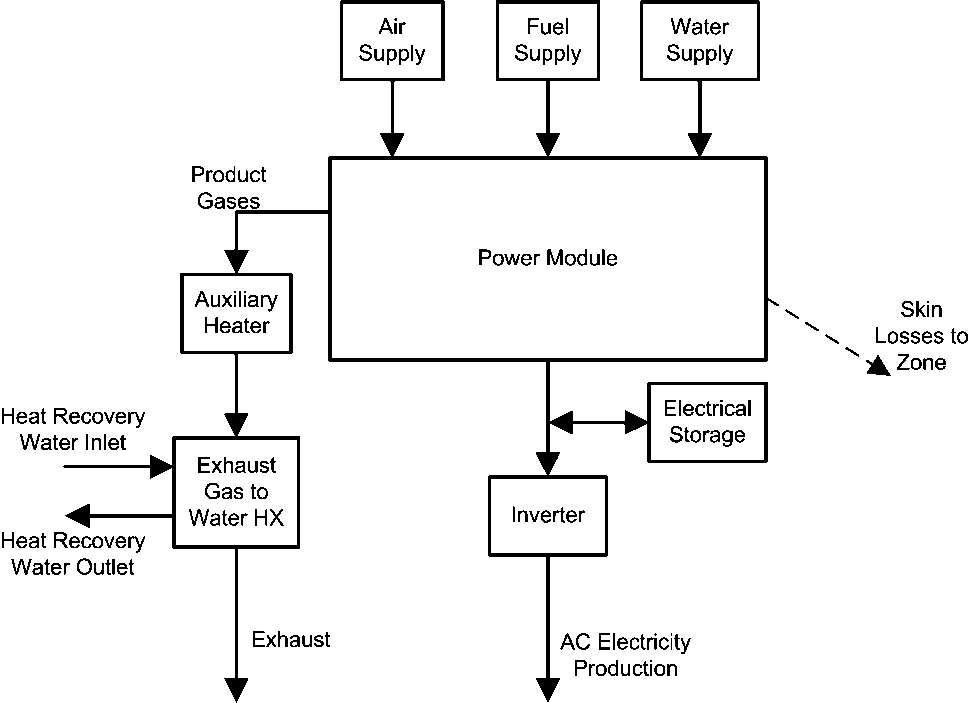
\includegraphics[width=0.9\textwidth, height=0.9\textheight, keepaspectratio=true]{media/image467.png}
\caption{Fuel cell subsystems. \protect \label{fig:fuel-cell-subsystems.}}
\end{figure}

Note that the FC model is formulated using the Lower Heating Value (LHV) of the fuel, whereas most other parts of EnergyPlus use the Higher Heating Value (HHV). LHV has important advantages over HHV in the context of the quality of heat recovered. While model coefficients for input performance descriptions are to be based on LHV, energy consumption and tariff calculations are also reported on HHV basis when using this model.

\subsubsection{Inputs}\label{inputs-12-003}

\paragraph{Field: Name}\label{field-name-13-002}

This field contains a unique name for the fuel cell.

\paragraph{Field: Power Module Name}\label{field-power-module-name}

This field contains the name of a \hyperref[generatorfuelcellpowermodule]{Generator:FuelCell:PowerModule} input object.

\paragraph{Field: Air Supply Name}\label{field-air-supply-name}

This field contains the name of a \hyperref[generatorfuelcellairsupply]{Generator:FuelCell:AirSupply} input object.

\paragraph{Field: Fuel Supply Name}\label{field-fuel-supply-name}

This field contains the name of a \hyperref[generatorfuelsupply]{Generator:FuelSupply} input object.

\paragraph{Field: Water Supply Name}\label{field-water-supply-name}

This field contains the name of a \hyperref[generatorfuelcellwatersupply]{Generator:FuelCell:WaterSupply} input object.

\paragraph{Field: Auxiliary Heater Name}\label{field-auxiliary-heater-name}

This field contains the name of a \hyperref[generatorfuelcellauxiliaryheater]{Generator:FuelCell:AuxiliaryHeater} input object.

\paragraph{Field: Heat Exchanger Name}\label{field-heat-exchanger-name-000}

This field contains the name of a \hyperref[generator-fuelcell-exhaustgastowaterheatexchanger]{Generator:FuelCell:ExhaustGasToWaterHeatExchanger} input object.

\paragraph{Field: Electrical Storage Name}\label{field-electrical-storage-name}

This field contains the name of a \hyperref[generatorfuelcellelectricalstorage]{Generator:FuelCell:ElectricalStorage} input object.

\paragraph{Field: Inverter Name}\label{field-inverter-name}

This field contains the name of a \hyperref[generatorfuelcellinverter]{Generator:FuelCell:Inverter} input object.

\paragraph{Field: Stack Cooler Name}\label{field-stack-cooler-name}

This field contains the name of a \hyperref[generatorfuelcellstackcooler]{Generator:FuelCell:StackCooler} input object. This is optional. The presence of a stack cooler distinguishes between SOFC and PEMFC with PEMFC operating at lower temperatures and requiring a separate subsystem to maintain stack temperatures.

An example input data file (IDF) entry for this object is provided below:

\begin{lstlisting}

Generator:FuelCell,
  FCT SOFC,                               !- Name
  FCT SOFC Power Module,     !- Power Module Name
  FCT SOFC Air Supply,         !- Air Supply Name
  FCT SOFC Fuel Supply,       !- Fuel Supply Name
  FCT SOFC Water Supply,     !- Water Supply Name
  FCT SOFC Auxiliary Heater,   !- Auxiliary Heater Name
  FCT SOFC Exhaust HX,         !- Heat Exchanger Name
  FCT SOFC Battery,               !- Electrical Storage Name
  FCT SOFC Inverter;             !- Inverter Name
\end{lstlisting}

\subsubsection{Outputs}\label{outputs-9-001}

The following output variables are available for the fuel cell model.

\begin{itemize}
\item
  Output:Variable,*,Generator Produced Electricity Rate,hourly; !- HVAC Average {[}W{]}
\item
  Output:Variable,*,Generator Produced Electricity Energy,hourly; !- HVAC Sum {[}J{]}
\item
  Output:Variable,*,Generator Produced Thermal Rate,hourly; !- HVAC Average {[}W{]}
\item
  Output:Variable,*,Generator Produced Thermal Energy,hourly; !- HVAC Sum {[}J{]}
\item
  Output:Variable,*,Generator Fuel HHV Basis Energy,hourly; !- HVAC Sum {[}J{]}
\item
  Output:Variable,*,Generator Fuel HHV Basis Rate,hourly; !- HVAC Average {[}W{]}
\item
  Output:Variable,*,Generator Fuel LHV Basis Energy,hourly; !- HVAC Sum {[}J{]}
\item
  Output:Variable,*,Generator Fuel Consumption Rate LHV Basis,hourly; !- HVAC Average {[}W{]}
\item
  Output:Variable,*,FuelCell Heat Loss Rate to Zone,hourly; !- HVAC Average {[}W{]}
\item
  Output:Variable,*,FuelCell Heat Loss Energy to Zone,hourly; !- HVAC Sum {[}J{]}
\item
  Output:Variable,*,FuelCell Convection Heat Loss Rate to Zone,hourly; !- HVAC Average {[}W{]}
\item
  Output:Variable,*,FuelCell Radiation Heat Loss Rate to Zone,hourly; !- HVAC Average {[}W{]}
\end{itemize}

\paragraph{Generator Produced Electricity Rate {[}W{]}}\label{generator-produced-electric-power-w-3}

This report is the net electrical power produced by the generator in watts.

\paragraph{Generator Produced Electricity Energy {[}J{]}}\label{generator-produced-electric-energy-j-3}

This report is the net electrical energy produced by the generator in joules. This output variable is also put on the meter for on-site production.

\paragraph{Generator Produced Thermal Rate {[}W{]}}\label{generator-produced-thermal-rate-w-3}

\paragraph{Generator Produced Thermal Energy {[}J{]}}\label{generator-produced-thermal-energy-j-3}

These are the rate and energy of thermal heat transferred from the engine to the heat recovery fluid in the coolant control volume.

\paragraph{Generator Fuel HHV Basis Energy {[}J{]}}\label{generator-fuel-hhv-basis-energy-j-3}

This is the energy used by the cogeneration device in terms of higher heating value in joules. This is the output variable is also put on the meter for natural gas.

\paragraph{Generator Fuel HHV Basis Rate {[}W{]}}\label{generator-fuel-hhv-basis-rate-w-3}

This is the rate of fuel energy use by the cogeneration device in terms of higher heating value in watts.

\paragraph{Generator Fuel LHV Basis Energy {[}J{]}}\label{generator-fuel-lhv-basis-energy-j-1}

This is the fuel energy used by the cogeneration device in terms of lower heating value in joules.

\paragraph{Generator Fuel Consumption Rate LHV Basis {[}W{]}}\label{generator-fuel-consumption-rate-lhv-basis-w}

This is the rate of fuel energy use by the cogeneration device in terms of lower heating value in watts.

\paragraph{Generator Zone Sensible Heat Transfer Rate {[}W{]}}\label{generator-zone-sensible-heat-transfer-rate-w-1}

This variable provides the results for the total rate of skin losses from the fuel cell to the surrounding zone.

\paragraph{Generator Zone Sensible Heat Transfer Energy {[}J{]}}\label{generator-zone-sensible-heat-transfer-energy-j-1}

This variable provides the results for the total energy in skin losses from the fuel cell to the surrounding zone.

\paragraph{Generator Zone Convection Heat Transfer Rate {[}W{]}}\label{generator-zone-convection-heat-transfer-rate-w-1}

This variable provides the results for the rate of skin losses in the form of surface convection heat transfer from the fuel cell to the surrounding zone.

\paragraph{Generator Zone Radiation Heat Transfer Rate {[}W{]}}\label{generator-zone-radiation-heat-transfer-rate-w-1}

This variable provides the results for the rate of skin losses in the form of radiation heat transfer from the fuel cell to the surrounding zone.

Using the FC model with DisplayAdvancedReportVariables (see Diagnostics object or use of operating system s environment variables) makes the following output variables available as listed in the RDD file. There are a large number of output variables that provide access to the inner workings of the model and individual subsystems that are not likely to be useful for the average user.

\begin{itemize}
\item
  HVAC,Average,Generator Air Inlet Temperature {[}C{]}
\item
  HVAC,Average,Generator Power Module Entering Air Temperature {[}C{]}
\item
  HVAC,Average,Generator Air Molar Flow Rate {[}kmol/s{]}
\item
  HVAC,Average,Generator Power Module Entering Air Enthalpy {[}W{]}
\item
  HVAC,Average,Generator Blower Electricity Rate {[}W{]}
\item
  HVAC,Sum,Generator Blower Electricity Energy {[}J{]}
\item
  HVAC,Average,Generator Blower Skin Heat Loss Rate {[}W{]}
\item
  HVAC,Average,Generator Fuel Inlet Temperature {[}C{]}
\item
  HVAC,Average,Generator Power Module Entering Fuel Temperature {[}C{]}
\item
  HVAC,Average,Generator Fuel Molar Flow Rate {[}kmol/s{]}
\item
  HVAC,Average,Generator Power Module Entering Fuel Enthalpy {[}W{]}
\item
  HVAC,Average,Generator Fuel Compressor Electricity Rate {[}W{]}
\item
  HVAC,Sum,Generator Fuel Compressor Electricity Energy {[}J{]}
\item
  HVAC,Average,Generator Fuel Compressor Skin Heat Loss Rate {[}W{]}
\item
  HVAC,Average,Generator Fuel Reformer Water Inlet Temperature {[}C{]}
\item
  HVAC,Average,Generator Power Module Entering Reforming Water Temperature {[}C{]}
\item
  HVAC,Average,Generator Fuel Reformer Water Molar Flow Rate {[}kmol/s{]}
\item
  HVAC,Average,Generator Fuel Reformer Water Pump Electricity Rate {[}W{]}
\item
  HVAC,Sum,Generator Fuel Reformer Water Pump Electricity Energy {[}J{]}
\item
  HVAC,Average,Generator Power Module Entering Reforming Water Enthalpy {[}W{]}
\item
  HVAC,Average,Generator Product Gas Temperature {[}C{]}
\item
  HVAC,Average,Generator Product Gas Enthalpy {[}W{]}
\item
  HVAC,Average,Generator Product Gas Molar Flow Rate {[}kmol/s{]}
\item
  HVAC,Average,Generator Product Gas Ar Molar Flow Rate {[}kmol/s{]}
\item
  HVAC,Average,Generator Product Gas CO2 Molar Flow Rate {[}kmol/s{]}
\item
  HVAC,Average,Generator Product Gas H2O Vapor Molar Flow Rate {[}kmol/s{]}
\item
  HVAC,Average,Generator Product Gas N2 Molar Flow Rate {[}kmol/s{]}
\item
  HVAC,Average,Generator Product Gas O2 Molar Flow Rate {[}kmol/s{]}
\item
  HVAC,Average,Generator Inverter Loss Power {[}W{]}
\item
  HVAC,Average,Generator Produced DC Electricity Rate {[}W{]}
\item
  HVAC,Average,Generator DC Power Efficiency {[]}
\item
  HVAC,Average,Generator Electric Storage Charge State {[}J{]}
\item
  HVAC,Average,Generator Produced DC Electricity Rate {[}W{]}
\item
  HVAC,Sum,Generator DC Storage Charging Energy {[}J{]}
\item
  HVAC,Average,Generator DC Storage Discharging Power {[}W{]}
\item
  HVAC,Sum,Generator DC Storage Discharging Energy {[}J{]}
\item
  HVAC,Average,Generator Ancillary AC Electricity Rate {[}W{]}
\item
  HVAC,Sum,Generator Ancillary AC Electricity Energy {[}J{]}
\item
  HVAC,Average,Generator Zone Sensible Heat Transfer Rate {[}W{]}
\item
  HVAC,Sum,Generator Zone Sensible Heat Transfer Energy {[}J{]}
\item
  HVAC,Average,Generator Zone Convection Heat Transfer Rate {[}W{]}
\item
  HVAC,Average,Generator Zone Radiation Heat Transfer Rate {[}W{]}
\item
  HVAC,Sum, Generator Fuel Cell Model Iteration Count {[]}
\item
  HVAC,Sum,Generator Root Solver Iteration Count {[]}
\end{itemize}

\paragraph{Generator Air Inlet Temperature {[}C{]}}\label{generator-air-inlet-temperature-c}

This variable provides the temperature of air supplied to the FC.

\paragraph{Generator Power Module Entering Air Temperature {[}C{]}}\label{generator-power-module-entering-air-temperature-c}

This variable provides the temperature of the air supplied to the power module after it has gone through the blower and received any heat recovered from other subsystems.

\paragraph{Generator Air Molar Flow Rate {[}kmol/s{]}}\label{generator-air-molar-flow-rate-kmols}

This variable provides the results for \({\dot N_{air}}\) , the flow rate of air into the FC.

\paragraph{Generator Power Module Entering Air Enthalpy {[}W{]}}\label{generator-power-module-entering-air-enthalpy-w}

This variable provides the results for \({\sum\limits_i {\left( {{{\dot N}_i} \cdot \left[ {{{\hat h}_i} - {\Delta_f}\hat h_i^0} \right]} \right)}_{air}}\) , which is the enthalpy flow in the air stream entering the power module relative to \SI{25}{\celsius}.

\paragraph{Generator Blower Electricity Rate {[}W{]}}\label{generator-blower-electric-power-w}

This variable provides the results for \({P_{blower - el}}\) , which is the electrical power used by the air supply blower.

\paragraph{Generator Blower Electricity Energy {[}J{]}}\label{generator-blower-electric-energy-j}

This variable provides the results for the energy used by the air supply blower. It is also added to the appropriate meters.

\paragraph{Generator Blower Skin Heat Loss Rate {[}W{]}}\label{generator-blower-skin-heat-loss-rate-w}

This variable provides the results for \({q_{blower - heat - loss}}\) , which is the rate of energy lost to the surroundings.

\paragraph{Generator Fuel Inlet Temperature {[}C{]}}\label{generator-fuel-inlet-temperature-c}

This variable provides the temperature of the fuel supplied to the FC.

\paragraph{Generator Power Module Entering Fuel Temperature {[}C{]}}\label{generator-power-module-entering-fuel-temperature-c}

This variable provides the temperature of the fuel supplied to the power module after it has gone through the compressor.

\paragraph{Generator Fuel Molar Flow Rate {[}kmol/s{]}}\label{generator-fuel-molar-flow-rate-kmols-1}

This variable provides the results for \({\dot N_{fuel}}\) , which is the flow rate of fuel into the FC.

\paragraph{Generator Power Module Entering Fuel Enthalpy {[}W{]}}\label{generator-power-module-entering-fuel-enthalpy-w}

This variable provides the results for \({\sum\limits_i {\left( {{{\dot N}_i} \cdot \left[ {{{\hat h}_i} - {\Delta_f}\hat h_i^0} \right]} \right)}_{fuel}}\) , which is the enthalpy flow in the fuel stream entering the power module relative to \SI{25}{\celsius}.

\paragraph{Generator Fuel Compressor Electricity Rate {[}W{]}}\label{generator-fuel-compressor-electric-power-w}

This variable provides the results for \({P_{comp - el}}\) , which is the electrical power used by the fuel supply compressor.

\paragraph{Generator Fuel Compressor Electricity Energy {[}J{]}}\label{generator-fuel-compressor-electric-energy-j}

This variable provides the results for the energy used by the fuel supply compressor. It is also added to the appropriate meters.

\paragraph{Generator Fuel Compressor Skin Heat Loss Rate {[}W{]}}\label{generator-fuel-compressor-skin-heat-loss-rate-w}

This variable provides the results for the rate of energy lost to the surroundings.

\paragraph{Generator Fuel Reformer Water Inlet Temperature {[}C{]}}\label{generator-fuel-reformer-water-inlet-temperature-c}

This variable provides the temperature of the water supplied to the FC for reforming.

\paragraph{Generator Power Module Entering Reforming Water Temperature {[}C{]}}\label{generator-power-module-entering-reforming-water-temperature-c}

This variable provides the temperature of the water supplied to the power module after it has gone through the pump.

\paragraph{Generator Fuel Reformer Water Molar Flow Rate {[}kmol/s{]}}\label{generator-fuel-reformer-water-molar-flow-rate-kmols}

This variable provides the results for \({\dot N_{water}}\) , which the flow rate of reforming water into the FC.

\paragraph{Generator Fuel Reformer Water Pump Electricity Rate {[}W{]}}\label{generator-fuel-reformer-water-pump-electric-power-w}

This variable provides the results for \({P_{pump - el}}\) , which is the electrical power used by the water pump.

\paragraph{Generator Fuel Reformer Water Pump Electricity Energy {[}J{]}}\label{generator-fuel-reformer-water-pump-electric-energy-j}

This variable provides the results for energy used by the water pump. It is also added to the appropriate meters.

\paragraph{Generator Power Module Entering Reforming Water Enthalpy {[}W{]}}\label{generator-power-module-entering-reforming-water-enthalpy-w}

This variable provides the results for \({\dot H_{liq - water}}\) which is the enthalpy flow of the water stream entering the power module relative to \SI{25}{\celsius}.

\paragraph{Generator Product Gas Temperature {[}C{]}}\label{generator-product-gas-temperature-c}

This variable provides the results for the temperature of the product gas stream leaving the fuel cell power module.

\paragraph{Generator Product Gas Enthalpy {[}W{]}}\label{generator-product-gas-enthalpy-w}

This variable provides the results for \({\sum\limits_i {\left( {{{\dot N}_i} \cdot \left[ {{{\hat h}_i} - {\Delta_f}\hat h_i^0} \right]} \right)}_{FCPM - cg}}\) , which is the enthalpy flow in the product gas stream leaving the power module relative to \SI{25}{\celsius}.

\paragraph{Generator Product Gas Molar Flow Rate {[}kmol/s{]}}\label{generator-product-gas-molar-flow-rate-kmols}

This variable provides the results for the flow rate of all the product gases leaving the fuel cell power module.

\paragraph{Generator Product Gas Ar Molar Flow Rate {[}kmol/s{]}}\label{generator-product-gas-ar-molar-flow-rate-kmols}

This variable provides the results for the flow rate of the argon gas leaving the fuel cell power module.

\paragraph{Generator Product Gas CO2 Molar Flow Rate {[}kmol/s{]}}\label{generator-product-gas-co2-molar-flow-rate-kmols}

This variable provides the results for the flow rate of the carbon dioxide gas leaving the fuel cell power module.

\paragraph{Generator Product Gas H2O Vapor Molar Flow Rate {[}kmol/s{]}}\label{generator-product-gas-h2o-vapor-molar-flow-rate-kmols}

This variable provides the results for the flow rate of the water gas leaving the fuel cell power module.

\paragraph{Generator Product Gas N2 Molar Flow Rate {[}kmol/s{]}}\label{generator-product-gas-n2-molar-flow-rate-kmols}

This variable provides the results for the flow rate of the nitrogen gas leaving the fuel cell power module.

\paragraph{Generator Product Gas O2 Molar Flow Rate {[}kmol/s{]}}\label{generator-product-gas-o2-molar-flow-rate-kmols}

This variable provides the results for the flow rate of the oxygen gas leaving the fuel cell power module.

\paragraph{Generator Inverter Loss Power {[}W{]}}\label{generator-inverter-loss-power-w}

This variable provides the results for the power losses associated with inefficiencies in the inverter.

\paragraph{Generator Produced DC Electricity Rate {[}W{]}}\label{generator-produced-dc-electric-power-w}

This variable provides the results for \({P_{el}}\) , which is the net DC electrical power produced by the fuel cell power module.

\paragraph{Generator DC Power Efficiency {[]}}\label{generator-dc-power-efficiency}

This variable provides the results for \({\varepsilon_{el}}\) , which is the electrical efficiency of the fuel cell power module.

\paragraph{Generator Electric Storage Charge State {[}J{]}}\label{generator-electric-storage-charge-state-j}

This variable provides the results for state of charge of the electrical storage device inside the fuel cell. Although the units are Joules, this is a state variable and is reported as an average rather than a sum.

\paragraph{Generator Produced DC Electricity Rate {[}W{]}}\label{generator-produced-dc-electric-power-w-1}

This variable provides the rate at which power was stored into the fuel cell's electrical storage subsystem.

\paragraph{Generator DC Storage Charging Energy {[}J{]}}\label{generator-dc-storage-charging-energy-j}

This variable provides the energy stored into the fuel cell's electrical storage subsystem.

\paragraph{Generator DC Storage Discharging Power {[}W{]}}\label{generator-dc-storage-discharging-power-w}

This variable provides the rate at which power was drawn from the fuel cell's electrical storage subsystem.

\paragraph{Generator DC Storage Discharging Energy {[}J{]}}\label{generator-dc-storage-discharging-energy-j}

This variable provides the energy drawn from the fuel cell's electrical storage subsystem.

\paragraph{Generator Ancillary AC Electricity Rate {[}W{]}}\label{generator-ancillary-ac-electric-power-w}

This variable provides the results for \({P_{el,ancillaries - AC}}\) , which is the rate at which ancillary devices within the power module use electricity supplied to the fuel cell by an external source.

\paragraph{Generator Ancillary AC Electricity Energy {[}J{]}}\label{generator-ancillary-ac-electric-energy-j}

This variable provides the results for the energy used by AC ancillaries. It is also added to the appropriate meters.

\paragraph{Generator Fuel Cell Model Iteration Count {[]}}\label{generator-fuel-cell-model-iteration-count}

This variable provides information on the numerical method used to calculate the FC model. EnergyPlus uses a sequential substitution iterative algorithm to solve the main heat balance equation for the FC model. This output variable indicates the number of iterations needed to converge.

\paragraph{Generator Root Solver Iteration Count {[]}}\label{generator-regula-falsi-iteration-count}

This variable provides information on the numerical method used to calculate product gas temperature as a function of the product gas's enthalpy. A root solver numerical method is used to invert the Shomate equation for enthalpy as a function of temperature. This output variable indicates the number of iterations needed for the root solver method to converge.

\paragraph{Generator Heat Recovery Exit Gas Temperature {[}C{]}}\label{generator-heat-recovery-exit-gas-temperature-c}

This is the temperature of the exiting gas for heat recovery in C.

\paragraph{Generator Heat Recovery Exit Gas H2O Vapor Fraction {[]}}\label{generator-heat-recovery-exit-gas-h2o-vapor-fraction}

This is the water vapor fraction in the exit gas.

\paragraph{Generator Heat Recovery Water Condensate Molar Flow Rate {[}kmol/s{]}}\label{generator-heat-recovery-water-condensate-molar-flow-rate-kmols}

This is the flow of condensed water in kmol/s.

\subsection{Generator:FuelCell:PowerModule}\label{generatorfuelcellpowermodule}

This object is used to describe the core power module subsystem of the FC. This includes the fuel cell stack, fuel reformer, and whatever ancillary devices are included inside. If the model has multiple FC generators that are of the exact same type, then only one of these objects is needed and all the \hyperref[generatorfuelcell]{Generator:FuelCell} can reference it. The model uses a number of curves to describe operating performance. Input data for specific models of FC are not yet available but will be produced by IEA Annex 42 and should be available in the future.

\subsubsection{Inputs}\label{inputs-13-003}

\paragraph{Field: Name}\label{field-name-14-001}

This field contains a unique name for the fuel cell power module subsystem.

\paragraph{Field: Efficiency Curve Mode}\label{field-efficiency-curve-mode}

This field is used to choose between different modes of inputting the electrical efficiency curve. There are two options available for this Field: Annex42 and Normalized . The Annex42 option indicates that the efficiency curves are not normalized and are used for the single size and type of FC product. The Normalized option indicates that the efficiency curves are normalized (as is standard practice in EnergyPlus) relative to a single rating point. In the Annex42 mode, the curves directly represent efficiency as a function of fuel use, but in the Normalized mode, the curves represent an efficiency modification that is applied to the efficiency at the rating point.

\paragraph{Field: Efficiency Curve Name}\label{field-efficiency-curve-name}

This field contains the name of a \hyperref[curvequadratic]{Curve:Quadratic} input object described elsewhere in the input file. The curve is a function of the net DC electric power, \({P_{el}}\) (W), produced by the power module and describes either the electrical efficiency or the how the efficiency is modified depending on the mode selected in the previous field. This quadratic curve is just one part of the entire parametric relation used to describe electrical efficiency \({\varepsilon_{el}}\) . For the Annex42 mode the full relation for efficiency is,

\begin{equation}
{\varepsilon_{el}} = \left[ {{\varepsilon_0} + {\varepsilon_1} \cdot {P_{el}} + {\varepsilon_2} \cdot P_{el}^2} \right] \cdot \left[ {1 - {N_{stops}} \cdot D} \right] \cdot \left[ {1 - (MAX(\int\limits_{} {dt - {t_{threshold}},0.0))}  \cdot L} \right]
\end{equation}

where the \hyperref[curvequadratic]{Curve:Quadratic} input object named in this field serves to define the quadratic portion in the first set of brackets. For the Normalized mode the full relation for efficiency is,

\begin{equation}
{\varepsilon_{el}} = \left[ {{\varepsilon_0} + {\varepsilon_1} \cdot \frac{{{P_{el}}}}{{{P_{nom}}}} + {\varepsilon_2} \cdot {{\left( {\frac{{{P_{el}}}}{{{P_{nom}}}}} \right)}^2}} \right] \cdot {\varepsilon_{nom}} \cdot \left[ {1 - {N_{stops}} \cdot D} \right] \cdot \left[ {1 - (MAX(\int\limits_0 {dt - {t_{threshold}},0.0))}  \cdot L} \right]
\end{equation}

where \({\varepsilon_{nom}}\) is the nominal electrical efficiency at the rating point \({P_{nom}}\) which are described in the next two fields. The Normalized mode may be more useful for a simulation study that needs to vary the capacity of the FC.

\paragraph{Field: Nominal Efficiency}\label{field-nominal-efficiency}

This field is used for the Normalized efficiency curve mode and provides the nominal efficiency \({\varepsilon_{nom}}\) (dimensionless) at the rating point. This field can be left blank if using the Annex42 mode.

\paragraph{Field: Nominal Electrical Power}\label{field-nominal-electrical-power}

This field is used for the Normalized efficiency curve mode and provides the nominal net DC electrical power produced \({P_{nom}}\) (W) at the rating point. This field can be left blank if using the Annex42 mode.

\paragraph{Field: Number of Stops at Start of Simulation}\label{field-number-of-stops-at-start-of-simulation}

This field is used to describe the number of times the FC has been cycled on and off prior to the start of the simulation. FC products might degrade as a result of starting and stopping the fuel cell stack, so the model includes terms to model the degradation effects of cycling FC units on and off. This is the initial value of the \({N_{stops}}\) \emph{\(_{}\)}term in the efficiency relation above.

\paragraph{Field: Cycling Performance Degradation Coefficient}\label{field-cycling-performance-degradation-coefficient}

This field is used to describe the fixed value representing the fractional performance degradation associated with each start and stop cycle. This is the value of \(D\) in the efficiency relations above. If there is no degradation from cycling, then D should be 0.0.

\paragraph{Field: Number of Run Hours at Beginning of Simulation}\label{field-number-of-run-hours-at-beginning-of-simulation}

This field is used to describe the amount of time the FC has been operating prior to the start of the simulation. FC products might degrade over time so the model includes terms to model the degradation effects of FC run time. This is the initial value of the integrated run time term \(\int\limits_0 {dt}\) .

\paragraph{Field: Accumulated Run Time Degradation Coefficient}\label{field-accumulated-run-time-degradation-coefficient}

This field is used to describe the fixed value representing the fractional performance degradation associated with the total amount of run time. This is the value of \(L\) in the efficiency relations above. If there is no degradation from run time, the L should be 0.0.

\paragraph{Field: Run Time Degradation Initiation Time Threshold}\label{field-run-time-degradation-initiation-time-threshold}

This field is used to describe the time period for which there is no degradation associated with the amount of run time. This provides the ability to model a system that initially operates without degradation for some period time before it starts to degrade. This is the value of \({t_{threshold}}\) in the efficiency relations above.

\paragraph{Field: Power Up Transient Limit}\label{field-power-up-transient-limit}

This field is used to describe the maximum allowable rate at which the fuel cell can increase the level of power it produces (W/s). This is a time derivative of the net DC electrical power used to limit how fast the FC can ramp up.

\paragraph{Field: Power Down Transient Limit}\label{field-power-down-transient-limit}

This field is used to describe the maximum allowable rate at which the fuel cell can decrease the level of power it produces (W/s). This is a time derivative of the net DC electrical power used to limit how fast the FC can ramp down.

\paragraph{Field: Start Up Time}\label{field-start-up-time}

This field is used to describe the length of time (seconds) of the start up period when the FC is turned on.

\paragraph{Field: Start Up Fuel}\label{field-start-up-fuel}

This field is used to describe the amount of fuel (kmol) used during the entire start up period. The fuel is the same type as what is described in the \hyperref[generatorfuelsupply]{Generator:FuelSupply} object elsewhere in the input file.

\paragraph{Field: Start Up Electricity Consumption}\label{field-start-up-electricity-consumption}

This field is used to describe the amount of electricity (Joules) used by ancillary equipment during the entire start up period.

\paragraph{Field: Start Up Electricity Produced}\label{field-start-up-electricity-produced}

This field is used to describe the amount of electricity (Joules) produced by the power module during the entire start up period.

\paragraph{Field: Shut Down Time}\label{field-shut-down-time}

This field is used to describe the length of time (seconds) of the shut down period.

\paragraph{Field: Shut Down Fuel}\label{field-shut-down-fuel}

This field is used to describe the amount of fuel (kmol) used during the entire shut down period. The fuel is the same type as what is described in the \hyperref[generatorfuelsupply]{Generator:FuelSupply} object elsewhere in the input file.

\paragraph{Field: Shut Down Electricity Consumption}\label{field-shut-down-electricity-consumption}

This field is used to describe the amount of electricity (J) used by ancillary equipment during the entire shut down period.

\paragraph{Field: Ancillary Electricity Constant Term}\label{field-ancillary-electricity-constant-term}

This field is used to describe the constant term, \(an{c_0}\) , in a relation that describes the AC electrical power used by ancillary equipment located inside the power module, \({P_{el,ancillaries - AC}}\) . The model uses this relation,

\begin{equation}
{P_{el,ancillaries - AC}} = an{c_0} + an{c_1} \cdot {\dot N_{fuel}}
\end{equation}

where \({\dot N_{fuel}}\) is the rate of fuel use in the power module (kmol/s).

\paragraph{Field: Ancillary Electricity Linear Term}\label{field-ancillary-electricity-linear-term}

This field is used to describe the linear term, \(an{c_1}\) , in the relation shown in the previous field.

\paragraph{Field: Skin Loss Calculation Mode}\label{field-skin-loss-calculation-mode}

This field is used to select the mode for how skin losses are modeled. Skin losses are heat energy lost from the power module and transferred to the surrounding thermal zone named in the following field. There are three alpha options to choose from: ConstantRate , UAForProcessGasTemperature , or QuadraticFunctionOfFuelRate. Enter ConstantRate in this field to model skin losses using a constant rate, e.g.~100 watts. Enter UAForProcessGasTemperature to model skin losses using a UA-Delta-T calculation method with the temperature difference determined by the power module's product gas temperature and the surrounding zone. Enter QuadraticFunctionOfFuelRate to model skin losses as a function of the rate of fuel use.

\paragraph{Field: Zone Name}\label{field-zone-name-8-000}

This field is used to describe the thermal zone that will receive skin and other heat losses from the FC. This should be the name of a Zone input object declared elsewhere in the input file.

\paragraph{Field: Skin Loss Radiative Fraction}\label{field-skin-loss-radiative-fraction-1}

This field is used to describe the portion of skin losses that are in the form of thermal radiation. This controls the radiative/convective split for the energy transferred to the zone by the FC.

\paragraph{Field: Constant Skin Loss Rate}\label{field-constant-skin-loss-rate}

This field is used to describe the constant rate of skin losses (W). This field is used with the ConstantRate mode. It can be left blank for other skin loss modes.

\paragraph{Field: Skin Loss U-Factor Times Area Term}\label{field-skin-loss-u-factor-times-area-term}

This field is used to describe the UA term (W/K). This field is used with the UAForProcessGasTemperature mode. It can be left blank for other skin loss modes. UA is the product of the overall heat transfer coefficient U and the area A.

\paragraph{Field: Skin Loss Quadratic Curve Name}\label{field-skin-loss-quadratic-curve-name}

This field is used to refer to the name of a quadratic curve object defined elsewhere in the input file. The quadratic curve should define skin heat loss rate as a function of the fuel use rate (kmol/s) so that,

\begin{equation}
{q_{skin - loss}} = {s_0} + {s_1} \cdot {\dot N_{fuel}} + {s_2} \cdot \dot N_{fuel}^2
\end{equation}

\paragraph{Field: Dilution Air Flow Rate}\label{field-dilution-air-flow-rate}

This field is used to describe the rate of dilution air (kmol/sec) drawn into, or through, the power module. This air stream may not be present in all FC products. It is used for limiting skin and stack heat losses and for strategies that mitigate potential safety issue were fuel gases to escape the stack.

\paragraph{Field: Stack Heat loss to Dilution Air}\label{field-stack-heat-loss-to-dilution-air}

This field is used to describe the rate at which the fuel cell stack adds energy to the dilution air stream. It is entered as a constant heat rate (W).

\paragraph{Field: Dilution Inlet Air Node Name}\label{field-dilution-inlet-air-node-name}

This field is used to describe the air node where the dilution air is drawn from. This would typically be the name of the air node associated with the thermal zone where the FC is located.

\paragraph{Field: Dilution Outlet Air Node Name}\label{field-dilution-outlet-air-node-name}

This field is used to describe the air node where the dilution air is exhausted to. This could be the inlets to a heat recovery ventilator or an exhaust node.

\paragraph{Field: Minimum Operating Point}\label{field-minimum-operating-point}

This field is used to describe the minimum operating point for the net DC electric power, \({P_{el}}\) (W).

\paragraph{Field: Maximum Operating Point}\label{field-maximum-operating-point}

This field is used to describe the maximum operating point for the net DC electric power, \({P_{el}}\) (W).

An example input data file (IDF) entry for this object is provided below:

\begin{lstlisting}

Generator:FuelCell:PowerModule,
  FCT SOFC Power Module,     !- Name
  Annex42,                                 !- Efficiency Curve Mode
  FCT Power Curve,                 !- Efficiency Curve Name
  0.354,                                     !- Nominal Efficiency
  3400,                                       !- Nominal Electrical Power {W}
  0,                                             !- Number of Stops at Start of Simulation
  0.0,                                         !- Cycling Performance Degradation Coefficient
  0,                                             !- Number of Run Hours at Beginning of Simulation {hr}
  0.0,                                         !- Accumulated Run Time Degradation Coefficient
  10000,                                     !- Run Time Degradation Initiation Time Threshold {hr}
  1.4,                                         !- Power Up Transient Limit {W/s}
  0.2,                                         !- Power Down Transient Limit {W/s}
  0.0,                                         !- Start Up Time {s}
  0.2,                                         !- Start Up Fuel {kmol}
  ,                                               !- Start Up Electricity Consumption {J}
  0.0,                                         !- Start Up Electricity Produced {J}
  0.0,                                         !- Shut Down Time {s}
  0.2,                                         !- Shut Down Fuel {kmol}
  ,                                               !- Shut Down Electricity Consumption {J}
  0.0,                                         !- Ancillary Electricity Constant Term
  0.0,                                         !- Ancillary Electricity Linear Term
  ConstantRate,                       !- Skin Loss Calculation Mode
  ZN_1_FLR_1_SEC_5,               !- Zone Name
  0.6392,                                   !- Skin Loss Radiative Fraction
  729,                                         !- Constant Skin Loss Rate {W}
  0.0,                                         !- Skin Loss U-Factor Times Area Term {W/K}
  ,                                               !- Skin Loss Quadratic Curve Name
  6.156E-3,                               !- Dilution Air Flow Rate {kmol/s}
  2307,                                       !- Stack Heat loss to Dilution Air {W}
  SOFC Air HR Inlet,             !- Dilution Inlet Air Node Name
  SOFC Air HR Outlet,           !- Dilution Outlet Air Node Name
  3010,                                       !- Minimum Operating Point {W}
  3728;                                       !- Maximum Operating Point {W}
\end{lstlisting}

\subsection{Generator:FuelCell:StackCooler}\label{generatorfuelcellstackcooler}

This object is optional and is used to define details needed to model the stack cooler on PEMFC.

\subsubsection{Field: Name}\label{field-name-15-001}

This field contains a unique name for the PEM fuel cell stack cooler

\subsubsection{Field: Heat Recovery Water Inlet Node Name}\label{field-heat-recovery-water-inlet-node-name-1}

This field contains the node name for the water inlet to the stack cooler.

\subsubsection{Field: Heat Recovery Water Outlet Node Nane}\label{field-heat-recovery-water-outlet-node-nane}

This field contains the node name for the water outlet from the stack cooler.

\subsubsection{Field: Nominal Stack Temperature}\label{field-nominal-stack-temperature}

This field contains the nominal stack operating temperature for the PEMFC, \(T_{stack}^o\) . This field and the next five provide values for use in the empirical equation for the rate of heat extracted from the fuel cell power module by the stack cooler using the following relation

\begin{equation}
{q_{s - cool}} = \left[ {{r_0} + {r_1}\left( {{T_{stack}} - T_{stack}^o} \right)} \right] \cdot \left[ {1 + {r_2}{P_{el}} + {r_3}P_{el}^2} \right]
\end{equation}

\subsubsection{Field: Actual Stack Temperature{]}}\label{field-actual-stack-temperature}

This field contains the actual stack operating temperature for the PEMFC, \({T_{stack}}\) .

\subsubsection{Field: Coefficient r0}\label{field-coefficient-r0}

This field contains the coefficient r\(_{0}\) in the equation above.

\subsubsection{Field: Coefficient r1}\label{field-coefficient-r1}

This field contains the coefficient r\(_{1}\) in the equation above.

\subsubsection{Field: Coefficient r2}\label{field-coefficient-r2}

This field contains the coefficient r\(_{2}\) in the equation above.

\subsubsection{Field: Coefficient r3}\label{field-coefficient-r3}

This field contains the coefficient r\(_{3}\) in the equation above.

\subsubsection{Field: Stack Coolant Flow Rate}\label{field-stack-coolant-flow-rate}

The stack cooler is assumed to have a closed water circulation loop that is used to extract heat from the stack and move it to a cogeneration heat exchanger and/or an air cooler. This field is used to enter the mass flow rate of coolant in this loop in kg/s.

\subsubsection{Field: Stack Cooler U-Factor Times Area Value}\label{field-stack-cooler-u-factor-times-area-value}

This is the heat transfer coefficient between the stack and the coolant in W/K.

\subsubsection{Field: Fs-cogen Adjustment Factor}\label{field-fs-cogen-adjustment-factor}

This field provides the value for an adjustment factor, \({F_{s - cogen}}\) , used in the following relation for the cogeneration heat transfer coefficient, \({\left( {UA} \right)_{s - cogen}}\) :

\begin{equation}
{\left( {UA} \right)_{s - cogen}} = {\left[ {\frac{1}{{{{\left( {hA} \right)}_{s - cogen}}}} + {F_{s - cogen}}} \right]^{ - 1}}
\end{equation}

\subsubsection{Field: Stack Cogeneration Exchanger Area}\label{field-stack-cogeneration-exchanger-area}

This field provides the value for the cogeneration heat exchanger area, \({A_{s - cogen}}\) in m2.

\subsubsection{Field: Stack Cogeneration Exchanger Nominal Flow Rate}\label{field-stack-cogeneration-exchanger-nominal-flow-rate}

This field provides the value in kg/s for \(\dot N_{s - cogen}^0\) in the following relation for the cogeneration heat exchanger convection coefficient, \({h_{s - cogen}}\) :

\begin{equation}
{h_{s - cogen}} = h_{s - cogen}^0 \cdot {\left( {\frac{{{{\dot N}_{s - cogen}}}}{{\dot N_{s - cogen}^0}}} \right)^{{n_s}}}
\end{equation}

\subsubsection{Field: Stack Cogeneration Exchanger Nominal Heat Transfer Coefficient}\label{field-stack-cogeneration-exchanger-nominal-heat-transfer-coefficient}

This field provides the value for \(h_{s - cogen}^0\) in the relation above for the cogeneration heat exchanger convection coefficient, \({h_{s - cogen}}\) in W/m2-K.

\subsubsection{Field: Stack Cogeneration Exchanger Nominal Heat Transfer Coefficient Exponent}\label{field-stack-cogeneration-exchanger-nominal-heat-transfer-coefficient-exponent}

This field provides the value for \({n_s}\) is the relation above for the cogeneration heat exchanger convection coefficient, \({h_{s - cogen}}\) .

\subsubsection{Field: Stack Cooler Pump Power}\label{field-stack-cooler-pump-power}

This field is the power used by the stack cooler's circulating pump in Watts. It is a constant power draw whenever the stack cooler is active.

\subsubsection{Field: Stack Cooler Pump Heat Loss Fraction}\label{field-stack-cooler-pump-heat-loss}

This field is the fraction of the pump power consumption that is lost to the surround zone.

\subsubsection{Field: Stack Air Cooler Fan Coefficient f0}\label{field-stack-air-cooler-fan-coefficient-f0}

This field and the next two are used to define coefficients for the following relation for the power used by the air-cooler's fan to dump excess heat into the surrounding zone:

\begin{equation}
{P_{s - air - el}} = {f_0} + {f_1} \cdot {q_{s - air}} + {f_2} \cdot q_{s - air}^2
\end{equation}

\subsubsection{Field: Stack Air Cooler Fan Coefficient f1}\label{field-stack-air-cooler-fan-coefficient-f1}

This field provides a value for the coefficient \emph{f\(_{1}\)} in the relation above.

\subsubsection{Field: Stack Air Cooler Fan Coefficient f2}\label{field-stack-air-cooler-fan-coefficient-f2}

This field provides a value for the coefficient \emph{f\(_{2}\)} in the relation above.

\subsection{Generator:FuelCell:AirSupply}\label{generatorfuelcellairsupply}

This object is used to define details of the air supply subsystem.

\subsubsection{Inputs}\label{inputs-14-003}

\paragraph{Field: Name}\label{field-name-16-001}

This field contains a unique name for the fuel cell air supply subsystem.

\paragraph{Field: Air Inlet Node Name}\label{field-air-inlet-node-name-1-000}

This field is used to define the air node where the inlet air stream is drawn from. If the FC uses outdoor air then the node named here should be designated an outdoor air node. If the FC draws air from its surroundings, then this would be the name of the air node associated with the thermal zone containing the FC.

\paragraph{Field: Blower Power Curve Name}\label{field-blower-power-curve-name}

This field contains the name of a \hyperref[curvecubic]{Curve:Cubic} input object described elsewhere in the input file. The curve provides the power used by the air blower (W) as a cubic function of the rate of air supply (kmol/s).

\begin{equation}
{P_{blower - el}} = {b_0} + {b_1} \cdot {\dot N_{air}} + {b_2} \cdot \dot N_{air}^2 + {b_3} \cdot \dot N_{air}^3
\end{equation}

\paragraph{Field: Blower Heat Loss Factor}\label{field-blower-heat-loss-factor}

This field describes the portion of blower electrical power that is lost to the surroundings. The rest of the energy is added to the air stream. A heat loss factor of 1.0 indicates that all the heat is lost to the surroundings and no energy is added to the air inlet stream.

\paragraph{Field: Air Supply Rate Calculation Mode}\label{field-air-supply-rate-calculation-mode}

This field describes how the model will calculate the air supply rate. There are three options to choose from: AirRatiobyStoics , QuadraticFunctionofElectricPower , and QuadraticFunctionofFuelRate. The choice will determine how the model calculates the rate of air and will depend on the formulations used to develop model input data. The choices are described in the next four fields.

\paragraph{Field: Stoichiometric Ratio}\label{field-stoichiometric-ratio}

This field describes the excess air ratio beyond stoichiometric air supply. This field is only used if the air supply rate calculation mode is AirRatiobyStoics. The total air supply ratio will be the value entered here plus 1.0. Thus if 1.0 is entered in this field, the total air flow will be 2.0 times what is needed to exactly match stoichiometry with the fuel supply.

\paragraph{Field: Air Rate Function of Electric Power Curve Name}\label{field-air-rate-function-of-electric-power-curve-name}

This field contains the name of a QuadraticCurve input object described elsewhere in the input file. This field is only used if the air supply rate calculation mode is QuadraticFunctionofElectricPower. The quadratic curve named here describes the first part of the relation below used to calculate the rate of inlet air, \({\dot N_{air}}\) (kmol/s). It is a quadratic function of the net DC electrical power, \({P_{el}}\) (W).

\begin{equation}
{\dot N_{air}} = \left[ {{a_0} + {a_1} \cdot {P_{el}} + {a_2} \cdot P_{el}^2} \right].\left[ {1 + {a_3} \cdot {T_{air}}} \right]
\end{equation}

\paragraph{Field: Air Rate Air Temperature Coefficient}\label{field-air-rate-air-temperature-coefficient}

This field is used to describe the air temperature coefficient, \({a_3}\), used to adjust inlet air flow rate in the relations for inlet air rate.

\paragraph{Field: Air Rate Function of Fuel Rate Curve Name}\label{field-air-rate-function-of-fuel-rate-curve-name}

This field contains the name of a \hyperref[curvequadratic]{Curve:Quadratic} input object described elsewhere in the input file. This field is only used if the air supply rate calculation mode is QuadraticFunctionofFuelRate. The quadratic curve named here describes the first part of the relation used to calculate the rate of inlet air, \({\dot N_{air}}\) (kmol/s). It is a quadratic function of the fuel flow rate, \({\dot N_{fuel}}\) .

 \({\dot N_{air}} = \left[ {{a_0} + {a_1} \cdot {{\dot N}_{fuel}} + {a_2} \cdot \dot N_{fuel}^2} \right].\left[ {1 + {a_3} \cdot {T_{air}}} \right]\)

\paragraph{Field: Air Intake Heat Recovery Mode}\label{field-air-intake-heat-recovery-mode}

This field is used to control how heat losses from three other subsystems within the FC may or may not be recovered by the air inlet. There are six possible choices for what to use in this Field: NoRecovery RecoverBurnerInverterStorage RecoverAuxiliaryBurner RecoverInverterandStorage RecoverInverter and RecoverElectricalStorage . If heat is recovered then that means that energy losses from those subsystems are added to the inlet air and fed back into the FC power module. The following table clarifies the meaning of the six possible choices.

% table 32
\begin{longtable}[c]{p{1.5in}p{1.5in}p{1.5in}p{1.5in}}
\caption{Air Intake Heat Recovery Mode Choices \label{table:air-intake-heat-recovery-mode-choices}} \tabularnewline
\toprule
Field Choice & Inverter Heat Losses Recovered? & Electrical Storage Heat Losses Recovered? & Auxiliary Heater Losses Recovered? \tabularnewline
\midrule
\endfirsthead

\caption[]{Air Intake Heat Recovery Mode Choices} \tabularnewline
\toprule
Field Choice & Inverter Heat Losses Recovered? & Electrical Storage Heat Losses Recovered? & Auxiliary Heater Losses Recovered? \tabularnewline
\midrule
\endhead

NoRecovery & No & No & No \tabularnewline
RecoverBurnerInverterStorage & Yes & Yes & Yes \tabularnewline
RecoverAuxiliaryBurner & No & No & Yes \tabularnewline
RecoverInverterandStorage & Yes & Yes & No \tabularnewline
RecoverInverter & Yes & No & No \tabularnewline
RecoverElectricalStorage & No & Yes & No \tabularnewline
\bottomrule
\end{longtable}

\paragraph{Field: Air Supply Constituent Mode}\label{field-air-supply-constituent-mode}

This field is used to choose between two different modes for describing the make up of the inlet air stream. There are two possible choices: AmbientAir or UserDefinedConstituents. Choosing the AmbientAir mode will automatically set the composition of air to be usual at: 77.28\% nitrogen, 20.73\% oxygen, 1.04\% water, 0.92\% argon, and 0.03\% carbon dioxide. Choosing UserDefinedConstituents allows the user to customize the make up the inlet air in the remaining fields.

\paragraph{Field: Number of UserDefined Constituents}\label{field-number-of-userdefined-constituents}

This field is used to describe the number of constituents in the inlet air. This field is only used if the air supply constituent mode is set to UserDefinedConstituents. The maximum number is 5.

The remaining fields in this object are repeating pairs of fields with one pair for each constituent and the same number as described in the previous field. The pairs consist of the name of the constituent followed by the molar fraction of that constituent.

\paragraph{Field: Constituent 1-5 Name}\label{field-constituent-1-5-name}

These fields describe the air stream constituents by name. The name field for each pair must be filled with one of these choices: CarbonDioxide , Nitrogen, Oxygen, Water, or Argon.

\paragraph{Field: Molar Fraction 1-5}\label{field-molar-fraction-1-5}

These fields describe the molar fraction of the air stream constituents. It is very important that the sum of the molar fractions add up to 1.0.

An example input data file (IDF) entry for this object is provided below:

\begin{lstlisting}

Generator:FuelCell:AirSupply,
  FCT SOFC Air Supply,         !- Name
  SOFC Air Inlet Node,         !- Air Inlet Node Name
  FCT Blower Power Curve,   !- Blower Power Curve Name
  1.0,                                         !- Blower Heat Loss Factor
  QuadraticFunctionofElectricPower,   !- Air Supply Rate Calculation Mode
  ,                                               !- Stoichiometric Ratio
  FCT Excess Air Ratio Curve,   !- Air Rate Function of Electric Power Curve Name
  2.83507E-3,                           !- Air Rate Air Temperature Coefficient
  ,                                               !- Air Rate Function of Fuel Rate Curve Name
  NoRecovery,                           !- Air Intake Heat Recovery Mode
  UserDefinedConstituents,   !- Air Supply Constituent Mode
  5,                                             !- Number of UserDefined Constituents
  Nitrogen,                               !- Constituent 1 Name
  0.7728,                                   !- Molar Fraction 1
  Oxygen,                                   !- Constituent 2 Name
  0.2073,                                   !- Molar Fraction 2
  Water,                                     !- Constituent 3 Name
  0.0104,                                   !- Molar Fraction 3
  Argon,                                     !- Constituent 4 Name
  0.0092,                                   !- Molar Fraction 4
  CarbonDioxide,                     !- Constituent 5 Name
  0.0003;                                   !- Molar Fraction 5
\end{lstlisting}

\subsection{Generator:FuelCell:WaterSupply}\label{generatorfuelcellwatersupply}

This object is used to provide details of the water supply subsystem. This water is used for steam reforming of the fuel and is not the same as the water used for thermal heat recovery.

\begin{lstlisting}
Generator:FuelCell:WaterSupply,
   A1, \field Name
           \required-field
           \reference FCWaterSupNames
   A2, \field Reformer Water Flow Rate Function of Fuel Rate Curve Name
           \type object-list
           \object-list QuadraticCurves
   A3, \field Reformer Water Pump Power Function of Fuel Rate Curve Name
           \type object-list
           \object-list QubicCurves
   N1, \field Pump Heat Loss Factor
   A4, \field Water Temperature Modeling Mode
           \type choice
           \key TemperatureFromAirNode
           \key TemperatureFromWaterNode
           \key TemperatureFromSchedule
           \key MainsWaterTemperature
   A5, \field Water Temperature Reference Node Name
   A6; \field Water Temperature Schedule Name
           \type object-list
           \object-list ScheduleNames
\end{lstlisting}

\subsubsection{Inputs}\label{inputs-15-003}

\paragraph{Field: Name}\label{field-name-17-000}

This field contains a unique name for the fuel cell water supply subsystem.

\paragraph{Field: Reformer Water Flow Rate Function of Fuel Rate Curve Name}\label{field-reformer-water-flow-rate-function-of-fuel-rate-curve-name}

This field contains the name of a \hyperref[curvequadratic]{Curve:Quadratic} input object described elsewhere in the input file. The curve provides the rate of water flow (kmol/sec) as a function of fuel flow rate (kmol/sec).

\begin{equation}
{\dot N_{liq - water}} = {w_0} + {w_1} \cdot {\dot N_{fuel}} + {w_2} \cdot \dot N_{fuel}^2
\end{equation}

If the unit does not use water for reforming then use a null quadratic where all the coefficients are 0.0.

\paragraph{Field: Reformer Water Pump Power Function of Fuel Rate Curve Name}\label{field-reformer-water-pump-power-function-of-fuel-rate-curve-name}

This field contains the name of a \hyperref[curvecubic]{Curve:Cubic} input object described elsewhere in the input file. The curve provides the power used by the water pump (W) as a cubic function of the rate of water supply (kmol/s).

\begin{equation}
{P_{pump - el}} = {p_0} + {p_1} \cdot {\dot N_{water}} + {p_2} \cdot \dot N_{water}^2 + {p_3} \cdot \dot N_{water}^3
\end{equation}

If the unit does not use water for reforming then use a null cubic where all the coefficients are 0.0.

\paragraph{Field: Pump Heat Loss Factor}\label{field-pump-heat-loss-factor}

This field describes the portion of pump electrical power that is lost to the surroundings. The rest of the energy is added to the water stream. A heat loss factor of 1.0 indicates that all the heat is lost to the surroundings and no energy is added to the water inlet stream.

\paragraph{Field: Water Temperature Modeling Mode}\label{field-water-temperature-modeling-mode}

This field describes how the model will determine the inlet temperature of the water stream. There are four options to choose from: TemperatureFromAirNode, TemperatureFromWaterNode, TemperatureFromSchedule, and MainsWaterTemperature. For the first two options, the temperature of the water inlet is determined by the temperature at the node named in the next field. For the third option, the temperature is determined by the schedule in the last field. Using the MainsWaterTemperature option requires also defining a separate \hyperref[sitewatermainstemperature]{Site:WaterMainsTemperature} input object elsewhere in the input file.

\paragraph{Field: Water Temperature Reference Node Name}\label{field-water-temperature-reference-node-name}

This field is used to define the node where the temperature of the inlet water stream is obtained. This can be either an air node or a water node.

\paragraph{Field: Water Temperature Schedule Name}\label{field-water-temperature-schedule-name}

This field is used to define the name of a schedule, defined elsewhere in the input file, that will be used to determine the temperature of the water inlet stream when using the TemperatureFromSchedule mode.

An example input data file (IDF) entry for this object is provided below:

\begin{lstlisting}

Generator:FuelCell:WaterSupply,
  FCT SOFC Water Supply,     !- Name
  Null Quadratic,                   !- Reformer Water Flow Rate Function of Fuel Rate Curve Name
  Null Cubic,                           !- Reformer Water Pump Power Function of Fuel Rate Curve Name
  0.0,                                         !- Pump Heat Loss Factor
  TemperatureFromAirNode,   !- Water Temperature Modeling Mode
  SOFC Air Inlet Node,         !- Water Temperature Reference Node Name
  ;                                               !- Water Temperature Schedule Name

  Curve:Quadratic,
  Null Quadratic,                   !- Name
  0.0,                                         !- Coefficient1 Constant
  0.0,                                         !- Coefficient2 x
  0.0,                                         !- Coefficient3 x**2
  -1.0E+10,                               !- Minimum Value of x
  1.0E+10;                                 !- Maximum Value of x

  Curve:Cubic,
  Null Cubic,                           !- Name
  0.0,                                         !- Coefficient1 Constant
  0.0,                                         !- Coefficient2 x
  0.0,                                         !- Coefficient3 x**2
  0.0,                                         !- Coefficient4 x**3
  -1.0E+10,                               !- Minimum Value of x
  1.0E+10;                                 !- Maximum Value of x
\end{lstlisting}

\subsection{Generator:FuelCell:AuxiliaryHeater}\label{generatorfuelcellauxiliaryheater}

This object is intended for modeling an auxiliary heater, however this portion of the model is not yet available in EnergyPlus. An auxiliary heater may be present in fuel cell products so that the unit can meet much higher thermal loads than would be possible using only cogeneration. This portion of the model will be added in the future once suitable cogeneration control capabilities are also available. The input fields are described for future reference but may change. The program still requires one of these objects be included even though the data are not yet used (so that internal data structures can be allocated).

\subsubsection{Inputs}\label{inputs-16-002}

\paragraph{Field: Name}\label{field-name-18-000}

This field contains a unique name for the fuel cell auxiliary heater subsystem.

\paragraph{Field: Excess Air Ratio}\label{field-excess-air-ratio}

This field describes the excess air ratio beyond stoichiometric air supply for the heater. The total air supply ratio will be the value entered here plus 1.0. Thus if 1.0 is entered in this field, the total air flow will be 2.0 times what is needed to exactly match stoichiometry with the fuel supply.

\paragraph{Field: Ancillary Power Constant Term}\label{field-ancillary-power-constant-term}

This field describes the constant term, \({x_0}\) , used to model the auxiliary burner's ancillary devices such as fans and ignition controls. The electrical power for ancillaries is calculated using,

\begin{equation}
{P_{el,aux - ancillaries}} = {x_0} + {x_1} \cdot {\dot N_{aux - fuel}}
\end{equation}

\paragraph{Field: Ancillary Power Linear Term}\label{field-ancillary-power-linear-term}

This field describes the linear term, \({x_1}\) , used to model the auxiliary burner's ancillary devices.

\paragraph{Field: Skin Loss U-Factor Times Area Value}\label{field-skin-loss-u-factor-times-area-value-1}

This field describes the UA term (W/K) for calculating skin losses in the auxiliary burner. UA is the product of the overall heat transfer coefficient U and the area A. The skin heat losses are calculated using,

\begin{equation}
{q_{aux - skin - losses}} = {(UA)_{aux}} \cdot ({T_{aux - mix}} - {T_{room}})
\end{equation}

where, \({T_{aux - mix}}\) is temperature of product gases leaving the auxiliary burner and includes the mixing of the product gases from the fuel cell power module. Thus, the input for UA should reflect this choice of reference temperature rather than an exterior surface temperature of the auxiliary burner.

\paragraph{Field: Skin Loss Destination}\label{field-skin-loss-destination}

This field describes the user's choice for what happens to the skin losses. There are two options: SurroundingZone and AirInletForFuelCell . Entering SurroundingZone will direct the model to put the lost energy into the surrounding thermal Zone named in the next field. Entering AirInletForFuelCell will direct the model to put the lost energy into the air inlet stream for the fuel cell to preheat that air.

\paragraph{Field: Zone Name to Receive Skin Losses}\label{field-zone-name-to-receive-skin-losses}

This field is used to determine the zone that will receive the skin losses. Enter the name of a Zone declared elsewhere in the input file. This field is only used if the SurroundingZone mode is used in the previous field.

\paragraph{Field: Heating Capacity Units}\label{field-heating-capacity-units}

This field describes the user's choice for how the capacity of the auxiliary heater will be defined. There are two options: Watts or kmol/s. Entering Watts will direct the program to use the next two fields to determine the maximum and minimum heating capacity. Entering kmol/s will direct the program to use the last two fields to determine the maximum and minimum heating capacities.

\paragraph{Field: Maximum Heating Capacity in Watts}\label{field-maximum-heating-capacity-in-watts}

This field is used to describe the maximum heating capacity of the auxiliary burner (W).

\paragraph{Field: Minimum Heating Capacity in Watts}\label{field-minimum-heating-capacity-in-watts}

This field is used to describe the minimum heating capacity of the auxiliary burner (W).

\paragraph{Field: Maximum Heating Capacity in Kmol per Second}\label{field-maximum-heating-capacity-in-kmol-per-second}

This field is used to describe the maximum fuel use rate for the auxiliary burner (kmol/s).

\paragraph{Field: Minimum Heating Capacity in Kmol per Second}\label{field-minimum-heating-capacity-in-kmol-per-second}

This field is used to describe the minimum fuel use rate for the auxiliary burner (kmol/s).

An example input data file (IDF) entry for this object is provided below:

\begin{lstlisting}

Generator:FuelCell:AuxiliaryHeater,
  FCT SOFC Auxiliary Heater,   !- Name
  0.0,                                         !- Excess Air Ratio
  0.0,                                         !- Ancillary Power Constant Term
  0.0,                                         !- Ancillary Power Linear Term
  0.5,                                         !- Skin Loss U-Factor Times Area Value
  SurroundingZone,                 !- Skin Loss Destination
  ZN_1_FLR_1_SEC_5,               !- Zone Name to Receive Skin Losses
  Watts,                                     !- Heating Capacity Units
  0.0,                                         !- Maximum Heating Capacity in Watts
  0.0,                                         !- Minimum Heating Capacity in Watts
  ,                                               !- Maximum Heating Capacity in Kmol per Second
  ;                                               !- Minimum Heating Capacity in Kmol per Second
\end{lstlisting}

\subsection{Generator:FuelCell:ExhaustGasToWaterHeatExchanger}\label{generator-fuelcell-exhaustgastowaterheatexchanger}

This object is used to describe the exhaust gas heat exchanger subsystem of the FC used to recovery thermal energy.

\paragraph{Field: Name}\label{field-name-19-000}

This field contains a unique name for the fuel cell power module subsystem.

\paragraph{Field: Heat Recovery Water Inlet Node Name}\label{field-heat-recovery-water-inlet-node-name-2}

This field contains the name of the node that connects the heat exchanger's inlet to the plant loop. This water is used for heat recovery.

\paragraph{Field: Heat Recovery Water Outlet Node Name}\label{field-heat-recovery-water-outlet-node-name-1}

This field contains the name of the node that connects the heat exchanger's outlet to the plant loop.

\paragraph{Field: Heat Recovery Water Maximum Flow Rate}\label{field-heat-recovery-water-maximum-flow-rate}

This field describes the design maximum flow rate of the heat recovery water (m\(^{3}\)/s). The value should match the design flow rate of the plant loop connected to the FC.

\paragraph{Field: Exhaust Outlet Air Node Name}\label{field-exhaust-outlet-air-node-name}

This field is used to determine which node will receive the exhaust air stream leaving the FC. This node will usually be outside and not be referenced elsewhere. However, if the exhaust stream is used in a heat recovery ventilator (as described in section 11 of the Annex 42 specification) then the node would be reference in the heat recovery ventilator object.

\paragraph{Field: Heat Exchanger Calculation Method}\label{field-heat-exchanger-calculation-method}

This field is used to direct how EnergyPlus will calculate heat exchanger performance. The Annex 42 model provides for four different methods of modeling the heat exchanger. The choices available for this field are: FixedEffectiveness (method 1 in Annex 42 specification), EmpiricalUAeff (method 2), FundementalUAeff (method 3), or Condensing (method 4). The remaining fields provide input data for the different methods. The heat exchanger correlations are described below.

\paragraph{Field: Method 1 Heat Exchanger Effectiveness}\label{field-method-1-heat-exchanger-effectiveness}

This field describes constant heat exchanger effectiveness, \({\varepsilon_{HX}}\) . This field is only used with the FixedEffectiveness mode, which corresponds to method 1 in the Annex 42 specification. For this mode, the heat exchange between the exhaust gases and the heat recovery water are calculated using,

\begin{equation}
{q_{HX}} = {\varepsilon_{HX}} \cdot {\left( {\dot N{{\hat c}_p}} \right)_{\min }} \cdot \left( {{T_{aux - mix}} - {T_{water,in}}} \right)
\end{equation}

where, \({\left( {\dot N{{\hat c}_p}} \right)_{\min }}\) is the minimum value of \({\left( {\dot N{{\hat c}_p}} \right)_{aux - mix}}\) and \({\left( {\dot N{{\hat c}_p}} \right)_{water}}\) .

\paragraph{Field: Method 2 Parameter hxs0}\label{field-method-2-parameter-hxs0}

This field describes the value of \(h{x_{s,0}}\) in the relation below for effective UA. This field is used with the EmpiricalUAeff mode, which corresponds to method 2 in the Annex 42 specification and with the Condensing mode, which corresponds to method 4 . This method uses the log mean temperature difference (LMTD) approach to calculate the heat exchange:

\begin{equation}
{q_{HX}} = {\left( {UA} \right)_{eff}} \cdot \frac{{\left( {{T_{aux - mix}} - {T_{water,out}}} \right) - \left( {{T_{HX - exh}} - {T_{water,in}}} \right)}}{{\ln \left( {\frac{{{T_{aux - mix}} - {T_{water,out}}}}{{{T_{HX - exh}} - {T_{water,in}}}}} \right)}}
\end{equation}

The user input in this field, and the next four fields, describe coefficients in an empirical relation for \({\left( {UA} \right)_{eff}}\) :

\begin{equation}
{\left( {UA} \right)_{eff}} = h{x_{s,0}} + h{x_{s,1}} \cdot {\dot N_{water}} + h{x_{s,2}} \cdot \dot N_{water}^2 + h{x_{s,3}} \cdot {\dot N_{aux - mix}} + h{x_{s,4}} \cdot \dot N_{aux - mix}^2
\end{equation}

\paragraph{Field: Method 2 Parameter hxs1}\label{field-method-2-parameter-hxs1}

This field describes the value of \(h{x_{s,1}}\) in the relation above for effective UA. This field is used with the EmpiricalUAeff mode, which corresponds to method 2 in the Annex 42 specification and with the Condensing mode, which corresponds to method 4 .

\paragraph{Field: Method 2 Parameter hxs2}\label{field-method-2-parameter-hxs2}

This field describes the value of \(h{x_{s,2}}\) in the relation above for effective UA. This field is used with the EmpiricalUAeff mode, which corresponds to method 2 in the Annex 42 specification and with the Condensing mode, which corresponds to method 4 .

\paragraph{Field: Method 2 Parameter hxs3}\label{field-method-2-parameter-hxs3}

This field describes the value of \(h{x_{s,3}}\) in the relation above for effective UA. This field is used with the EmpiricalUAeff mode, which corresponds to method 2 in the Annex 42 specification and with the Condensing mode, which corresponds to method 4 .

\paragraph{Field: Method 2 Parameter hxs4}\label{field-method-2-parameter-hxs4}

This field describes the value of \(h{x_{s,4}}\) in the relation above for effective UA. This field is used with the EmpiricalUAeff mode, which corresponds to method 2 in the Annex 42 specification and with the Condensing mode, which corresponds to method 4 .

\paragraph{Field: Method 3 h0Gas Coefficient}\label{field-method-3-h0gas-coefficient}

This field describes the value of \(h_{gas}^0\) in the relation below. This field is only used with the FundementalUAeff mode, which corresponds to method 3 in the Annex 42 specification. For this mode, the heat exchange is calculated using the LMTD method, but the effective UA is determined using:

\begin{equation}
{\left( {UA} \right)_{eff}} = {\left[ {\frac{1}{{{{\left( {hA} \right)}_{gas}}}} + \frac{1}{{{{(hA)}_{water}}}} + {F_{HX}}} \right]^{ - 1}}
\end{equation}

where,

\({F_{HX}}\) is an adjustment factor,

\({h_{gas}} = h_{gas}^0 \cdot {\left( {\frac{{{{\dot N}_{gas}}}}{{\dot N_{gas}^0}}} \right)^n}\) ,

\begin{equation}
{h_{water}} = h_{water}^0 \cdot {\left( {\frac{{{{\dot N}_{water}}}}{{\dot N_{water}^0}}} \right)^m}
\end{equation}

\paragraph{Field: Method 3 NdotGasRef Coefficient}\label{field-method-3-ndotgasref-coefficient}

This field describes the value of \(\dot N_{gas}^0\) in the relation above. This field is only used with the FundementalUAeff mode, which corresponds to method 3 in the Annex 42 specification.

\paragraph{Field: Method 3 n Coefficient}\label{field-method-3-n-coefficient}

This field describes the value of \(n\) in the relation above. This field is only used with the FundementalUAeff mode, which corresponds to method 3 in the Annex 42 specification.

\paragraph{Field: Method 3 Gas Area}\label{field-method-3-gas-area}

This field describes the value of \({A_{gas}}\) in the relation above. This field is only used with the FundementalUAeff mode, which corresponds to method 3 in the Annex 42 specification.

\paragraph{Field: Method 3 h0 Water Coefficient}\label{field-method-3-h0-water-coefficient}

This field describes the value of \(h_{water}^0\) in the relation above. This field is only used with the FundementalUAeff mode, which corresponds to method 3 in the Annex 42 specification.

\paragraph{Field: Method 3 N dot Water ref Coefficient}\label{field-method-3-n-dot-water-ref-coefficient}

This field describes the value of \(\dot N_{water}^0\) in the relation above. This field is only used with the FundementalUAeff mode, which corresponds to method 3 in the Annex 42 specification.

\paragraph{Field: Method 3 m Coefficient}\label{field-method-3-m-coefficient}

This field describes the value of \(m\) in the relation above. This field is only used with the FundementalUAeff mode, which corresponds to method 3 in the Annex 42 specification.

\paragraph{Field: Method 3 Area Water Coefficient}\label{field-method-3-area-water-coefficient}

This field describes the value of \({A_{water}}\) in the relation above. This field is only used with the FundementalUAeff mode, which corresponds to method 3 in the Annex 42 specification.

\paragraph{Field: Method 3 F Adjustment Factor}\label{field-method-3-f-adjustment-factor}

This field describes the value of \({F_{HX}}\) in the relation above. This field is only used with the FundementalUAeff mode, which corresponds to method 3 in the Annex 42 specification.

\paragraph{Field: Method 4 hxl1 Coefficient}\label{field-method-4-hxl1-coefficient}

This field describes the value of \(h{x_{l,1}}\) in the relation below for the rate of condensation of water from the gas stream, \({\dot N_{{H_2}O - cond}}\) . This field is only used with the Condensing mode, which corresponds to method 4 in the Annex 42 specification. This method uses a modified version of the LMTD approach to calculate heat exchange:

\begin{equation}
{q_{HX}} = {\left( {UA} \right)_{eff}} \cdot \frac{{\left( {{T_{aux - mix}} - {T_{water,out}}} \right) - \left( {{T_{HX - exh}} - {T_{water,in}}} \right)}}{{\ln \left( {\frac{{{T_{aux - mix}} - {T_{water,out}}}}{{{T_{HX - exh}} - {T_{water,in}}}}} \right)}} + {\dot N_{{H_2}O - cond}} \cdot {\hat h_{fg}}
\end{equation}

where,

\begin{equation}
{\dot N_{{H_2}O - cond}} = \left( {{T_{cond - threshold}} - {T_{water,in}}} \right) \cdot \left[ {h{x_{l,1}} \cdot \left( {\frac{{{{\dot N}_{{H_2}O}}}}{{{{\dot N}_{aux - mix}}}}} \right) + h{x_{l,2}} \cdot {{\left( {\frac{{{{\dot N}_{{H_2}O}}}}{{{{\dot N}_{aux - mix}}}}} \right)}^2}} \right]
\end{equation}

\paragraph{Field: Method 4 hxl2 Coefficient}\label{field-method-4-hxl2-coefficient}

This field describes the value of \(h{x_{l,2}}\) in the relation above for the rate of condensation of water from the gas stream, \({\dot N_{{H_2}O - cond}}\) . This field is only used with the Condensing mode, which corresponds to method 4 in the Annex 42 specification.

\paragraph{Field: Method 4 Condensation Threshold}\label{field-method-4-condensation-threshold}

This field describes the value of \({T_{cond - threshold}}\) in the relation above for the rate of condensation of water from the gas stream, \({\dot N_{{H_2}O - cond}}\) . This field is only used with the Condensing mode, which corresponds to method 4 in the Annex 42 specification.

An example input data file (IDF) entry for this object is provided below:

\begin{lstlisting}

Generator:FuelCell:ExhaustGasToWaterHeatExchanger,
  FCT SOFC Exhaust HX,         !- Name
  Small SOFC Heat Rec Inlet Node,   !- Heat Recovery Water Inlet Node Name
  Small SOFC Heat Rec Outlet Node,   !- Heat Recovery Water Outlet Node Name
  0.0004,                                   !- Heat Recovery Water Maximum Flow Rate {m3/s}
  SOFC Air Outlet Node,       !- Exhaust Outlet Air Node Name
  CONDENSING,                           !- Heat Exchanger Calculation Method
  ,                                               !- Method 1 Heat Exchanger Effectiveness
  83.1,                                       !- Method 2 Parameter hxs0
  4798,                                       !- Method 2 Parameter hxs1
  -138E+3,                                 !- Method 2 Parameter hxs2
  -353.8E+3,                             !- Method 2 Parameter hxs3
  5.15E+8,                                 !- Method 2 Parameter hxs4
  ,                                               !- Method 3 h0Gas Coefficient
  ,                                               !- Method 3 NdotGasRef Coefficient
  ,                                               !- Method 3 n Coefficient
  ,                                               !- Method 3 Gas Area
  ,                                               !- Method 3 h0 Water Coefficient
  ,                                               !- Method 3 N dot Water ref Coefficient
  ,                                               !- Method 3 m Coefficient
  ,                                               !- Method 3 Area Water Coefficient
  ,                                               !- Method 3 F Adjustment Factor
  -1.96E-4,                               !- Method 4 hxl1 Coefficient
  3.1E-3,                                   !- Method 4 hxl2 Coefficient
  35.0;                                       !- Method 4 Condensation Threshold {C}
\end{lstlisting}

\subsection{Generator:FuelCell:ElectricalStorage}\label{generatorfuelcellelectricalstorage}

This object is used to describe the electrical storage subsystem for the FC. The electrical storage model is a very simple constrained bucket model. Future developments made add additional models for battery systems. Note that this electrical storage is embedded within the FC device.

\subsubsection{Inputs}\label{inputs-17-000}

\paragraph{Field: Name}\label{field-name-20}

This field contains a unique name for the fuel cell electrical storage subsystem.

\paragraph{Field: Choice of Model}\label{field-choice-of-model}

This field is used to direct how EnergyPlus will model electrical storage. The only choice currently available is SimpleEfficiencyWithConstraints, which should be entered in this field. Future developments may expand the number of models available for electrical storage.

\paragraph{Field: Nominal Charging Energetic Efficiency}\label{field-nominal-charging-energetic-efficiency}

This field describes the value of \({\varepsilon_{charge}}\) in the relation for the State of Charge, \(Q_{battery}^{t + \Delta t}\) :

\begin{equation}
Q_{battery}^{t + \Delta t} = Q_{battery}^t + {P_{battery - charge}} \cdot {\varepsilon_{charge}} \cdot \Delta t
\end{equation}

This is the energetic efficiency of charging the storage device. A value of 1.0 means that the storage device does not lose any energy when charging. Note that the model can recover the lost energy into the air supply intake.

\paragraph{Field: Nominal Discharging Energetic Efficiency}\label{field-nominal-discharging-energetic-efficiency-1}

This field describes the value of \({\varepsilon_{discharge}}\) in the relation for the State of Charge, \(Q_{battery}^{t + \Delta t}\) :

\begin{equation}
Q_{battery}^{t + \Delta t} = Q_{battery}^t + \frac{{{P_{battery - discharge}} \cdot \Delta t}}{{{\varepsilon_{discharge}}}}
\end{equation}

This is the energetic efficiency of discharging the storage device. A value of 1.0 means that the storage device does not lose any energy when discharging. Note that the model can recover the lost energy into the air supply intake.

\paragraph{Field: Simple Maximum Capacity}\label{field-simple-maximum-capacity}

This field describes the maximum amount of electrical energy that can be stored in the device (J).

\paragraph{Field: Simple Maximum Power Draw}\label{field-simple-maximum-power-draw}

This field describes the maximum rate at which electrical power can be discharged from the storage device (W).

\paragraph{Field: Simple Maximum Power Store}\label{field-simple-maximum-power-store}

This field describes the maximum rate at which electrical power can charge the storage device (W).

\paragraph{Field: Initial Charge State}\label{field-initial-charge-state}

This field describes the value for the initial state of charge (J). This allows the storage device to contain some amount of stored electricity at the beginning of the simulation period.

An example input data file (IDF) entry for this object is provided below:

\begin{lstlisting}

Generator:FuelCell:ElectricalStorage,
  FCT SOFC Battery,               !- Name
  SimpleEfficiencyWithConstraints,   !- Choice of Model
  1.0,                                         !- Nominal Charging Energetic Efficiency
  1.0,                                         !- Nominal Discharging Energetic Efficiency
  0,                                             !- Simple Maximum Capacity {J}
  0,                                             !- Simple Maximum Power Draw {W}
  0,                                             !- Simple Maximum Power Store {W}
  0;                                             !- Initial Charge State {J}
\end{lstlisting}

\subsection{Generator:FuelCell:Inverter}\label{generatorfuelcellinverter}

This object is used to describe the power condition unit subsystem of the FC. This object models an inverter system contained within a fuel cell system that converts from direct current (DC) to alternating current (AC).

\subsubsection{Inputs}\label{inputs-18-000}

\paragraph{Field: Name}\label{field-name-21}

This field contains a unique name for the fuel cell inverter subsystem.

\paragraph{Field: Inverter Efficiency Calculation Mode}\label{field-inverter-efficiency-calculation-mode}

This field is used to direct how EnergyPlus will calculate the inverter efficiency. There are two possible choices: Constant or Quadratic .

\paragraph{Field: Inverter Efficiency}\label{field-inverter-efficiency-1}

This field describes the value for inverter efficiency when using the \textbf{Constant} mode.

\paragraph{Field: Efficiency Function of DC Power Curve Name}\label{field-efficiency-function-of-dc-power-curve-name}

This field names a \hyperref[curvequadratic]{Curve:Quadratic} object defined elsewhere in the input file. The curve determines inverter efficiency as a function of the DC power entering the inverter as follows:

\begin{equation}
{\eta_{PCU}} = {u_0} + {u_1} \cdot {P_{PCU - in}} + {u_2} \cdot P_{PCU - in}^2
\end{equation}

An example input data file (IDF) entry for this object is provided below:

\begin{lstlisting}

Generator:FuelCell:Inverter,
  FCT SOFC Inverter,             !- Name
  Quadratic,                             !- Inverter Efficiency Calculation Mode
  ,                                               !- Inverter Efficiency
  FCT Inverter Quadratic;   !- Efficiency Function of DC Power Curve Name


  Curve:Quadratic,
  FCT Inverter Quadratic,   !- Name
  0.560717,                               !- Coefficient1 Constant
  1.24019E-4,                           !- Coefficient2 x
  -2.01648E-8,                         !- Coefficient3 x**2
  -1.0E+10,                               !- Minimum Value of x
  1.0E+10;                                 !- Maximum Value of x
\end{lstlisting}

\subsection{Generator:FuelSupply}\label{generatorfuelsupply}

This object is used to define details of the fuel supply for certain generators. This object allows the user to describe a wide array of possible fuel mixtures. The program contains data and internal methods to calculate the properties of the various mixtures of gaseous fuels. The program will calculate the Lower Heating Value (LHV), Higher Heating Value (HHV), and molecular weight for the fuel mixture. The fuel properties are then use by both fuel cell and Micro CHP models. Results of the gas phase thermochemistry modeling are also reported in the EIO file.

In addition to gaseous mixtures, the Micro CHP model is able to use generic liquid fuels and this object is used to describe the properties.

Note that the fuel consumption metering is currently handled by the Natural Gas meter. So no matter what fuel mixture is defined in this object, the aggregated reports from EnergyPlus meters for (natural) Gas will include the fuel used for the generator (with the Joule content based on HHV).

\subsubsection{Inputs}\label{inputs-19-000}

\paragraph{Field: Name}\label{field-name-22}

This field contains a unique name for the fuel cell fuel supply subsystem.

\paragraph{Field: Fuel Temperature Modeling Mode}\label{field-fuel-temperature-modeling-mode}

This field describes how the model will determine the temperature of the fuel. There are two options for this field to choose from: TemperatureFromAirNode and Scheduled. If this field contains TemperatureFromAirNode then the fuel is modeled as having the same temperature as the air node that is named in the next field. If this field contains Scheduled then the fuel is modeled as having the temperature described in a schedule defined elsewhere in the input file.

\paragraph{Field: Fuel Temperature Reference Node Name}\label{field-fuel-temperature-reference-node-name}

This field contains the name of the air node used to obtain the inlet temperature of the fuel. This field is only used if the Fuel Temperature Modeling Mode is set to TemperatureFromAirNode.

\paragraph{Field: Fuel Temperature Schedule Name}\label{field-fuel-temperature-schedule-name}

This field contains the name of a temperature schedule defined elsewhere in the input file. This field is only used if the Fuel Temperature Modeling Mode is set to Scheduled. The temperature of the fuel inlet will be obtained from the schedule.

\paragraph{Field: Compressor Power Function of Fuel Rate Curve Name}\label{field-compressor-power-function-of-fuel-rate-curve-name}

This field contains the name of a \hyperref[curvecubic]{Curve:Cubic} input object described elsewhere in the input file. The curve provides the electrical power used by the fuel compressor (W) as a cubic function of the rate of fuel supply (kmol/s).

\begin{equation}
{P_{comp - el}} = {c_0} + {c_1} \cdot {\dot N_{fuel}} + {c_2} \cdot \dot N_{fuel}^2 + {c_3} \cdot \dot N_{fuel}^3
\end{equation}

\paragraph{Field: Compressor Heat Loss Factor}\label{field-compressor-heat-loss-factor}

This field describes the portion of the compressor electrical power that is lost to the surroundings. The rest of the energy is added to the fuel stream. A heat loss factor of 1.0 indicates that all the heat is lost to the surroundings and no energy is added to the fuel inlet stream.

\paragraph{Field: Fuel Type}\label{field-fuel-type-3}

Choose between GaseousConstituents or LiquidGeneric .

\paragraph{Field: Liquid Generic Fuel Lower Heating Value}\label{field-liquid-generic-fuel-lower-heating-value}

For fuel type LiquidGeneric, this field is used to enter the lower heating value of the fuel in units of kJ/kg.

\paragraph{Field: Liquid Generic Fuel Higher Heating Value}\label{field-liquid-generic-fuel-higher-heating-value}

For fuel type LiquidGeneric, this field is used to enter the higher heating value of the fuel in units of kJ/kg.

\paragraph{Field: Liquid Generic Fuel Molecular Weight}\label{field-liquid-generic-fuel-molecular-weight}

For fuel type LiquidGeneric, this field is used to enter the molecular weight of the fuel in units of g/mol.

\paragraph{Field: Liquid Generic Fuel CO2 Emission Factor}\label{field-liquid-generic-fuel-co2-emission-factor}

This field is not used. This part of the Annex 42 model was not implemented in EnergyPlus; see the \hyperref[fuelfactors]{FuelFactors} object.

\paragraph{Field: Number of Constituents in Gaseous Constituent Fuel Supply}\label{field-number-of-constituents-in-gaseous-constituent-fuel-supply}

This field is used to describe the number of constituents in the inlet fuel supply. The maximum number of different types of constituents is currently set to 12.

The remaining fields in this object are repeating pairs of fields with one pair for each constituent and the same number as described in the previous field. The field set pairs consist of the name of the constituent followed by the molar fraction of that constituent.

\paragraph{Field: Constituent 1-12 Name}\label{field-constituent-1-12-name}

These fields describe the fuel stream constituents by name. The name field for each pair must be filled with one of these 14 choices: CarbonDioxide , Nitrogen , Oxygen , Water , Argon , Hydrogen , Methane , Ethane , Propane , Butane , Pentane , Hexane , Methanol , and Ethanol . No other fuel constituents can currently be modeled. The properties of the constituents are already contained inside the program as provided in the Annex 42 model specification.

\paragraph{Field: Constituent 1-12 Molar Fraction}\label{field-constituent-1-12-molar-fraction}

These fields describe the molar fraction of the fuel stream constituents. It is very important that the sum of the molar fractions add up to 1.0.

\subsubsection{Outputs}\label{outputs-10-001}

In addition to the following output variables, the resulting fuel heating values are also reported to the eio file.

HVAC,Average,Generator Fuel Compressor Electricity Rate {[}W{]}

HVAC,Sum,Generator Fuel Compressor Electricity Energy {[}J{]}

HVAC,Average,Generator Fuel Compressor Skin Heat Loss Rate {[}W{]}

\paragraph{Generator Fuel Compressor Electricity Rate {[}W{]}}\label{generator-fuel-compressor-electric-power-w-1}

This is the rate of energy use by the gas compressor, if any, that provides fuel at a higher pressure.

\paragraph{Generator Fuel Compressor Electricity Energy {[}J{]}}\label{generator-fuel-compressor-electric-energy-j-1}

This is the energy used by the gas compressor, if any, that provides fuel at a higher pressure.

\paragraph{Generator Fuel Compressor Skin Heat Loss Rate {[}W{]}}\label{generator-fuel-compressor-skin-heat-loss-rate-w-1}

Convective heat gains to zone from gas compressor, if any, that provides fuel at a higher pressure.

\subsection{Photovoltaic Generators}\label{photovoltaic-generators}

EnergyPlus offers different options for predicting the electricity produced by solar electric photovoltaic (PV) panels. The three different options are Simple , Equivalent One-Diode and Sandia and the choice will determine the mathematical models used to determine energy production. The first allows the user to input an arbitrary efficiency. The other two models use empirical relationships to predict PV operating performance based on many environmental variables such as cell temperature. The PV models can be used with either normal PV modules or as part of a hybrid photovoltaic/thermal (PVT) flat plat collector.

The generator is connected to an Electric Load Center. The PV models refer to surface input objects defined elsewhere in the input file. This object describes an array that is attached to a surface object in order to describe its orientation and to access results of the solar insolation calculations. These can be either Heat Transfer or Shading objects (see Surfaces). This will define the orientation of the solar panel for the detailed models and also the area for the simple model. The exposure of that surface to incident solar radiation is calculated using the full set of models in EnergyPlus that are used to account for solar thermal loads arising from building windows and walls. Therefore the incident solar radiation is calculated to include the effects of shading and reflections from other surfaces declared in the input file. In addition to the output variables associated with PV models, there are numerous related output variables available for the surfaces including: `Surface Outside Face Sunlit Area', `Surface Outside Face Sunlit Fraction', `Surface Outside Face Incident Solar Radiation Rate per Area', `Surface Outside Face Incident Beam Solar Radiation Rate per Area', `Surface Outside Face Incident Sky Diffuse Solar Radiation Rate per Area', `Surface Outside Face Incident Ground Diffuse Solar Radiation Rate per Area', `Surface Outside Face Beam Solar Incident Angle Cosine Value', `Surface Outside Face Incident Sky Diffuse Ground Reflected Solar Radiation Rate per Area', `Surface Outside Face Incident Sky Diffuse Surface Reflected Solar Radiation Rate per Area', `Surface Outside Face Incident Beam To Beam Reflected From Surfaces Solar Radiation Rate per Area', `Surface Outside Face Incident Beam To Diffuse Surface Reflected Solar Radiation Rate per Area', and 'Surface Outside Face Incident Beam To Diffuse Ground Reflected Solar Radiation Rate per Area. Note that it is possible to define a PV array area that doesn't conform to the surface area (i.e. model a PV array area that is larger or smaller than what is available on the surface) so it is the users responsibility to not over-specify area when determining how many modules will fit onto a surface. However this type of input is allowed.

EnergyPlus does not include models for ancillary equipment for a PV array including charge controllers or power-point trackers. The operation of the entire electrical system that must go along with a PV array is not currently modeled in EnergyPlus and is therefore assumed to operate in ideal ways. The PV production models do not resolve voltage and current, only power (and energy). Electricity production is metered based on the output of the inverter. Output results are available before and after the inverter. One assumption is that the array is assumed to be always operating at the maximum power point. Energy production is based on the assumption that the quasi-steady power prediction is constant and continuous over the simulation timestep.

For a variety of reasons, actual installations of photovoltaics are often observed to exhibit system-level problems that significantly reduce electricity production. Therefore this modeling should be considered a method of bracketing the upper end of electricity production rather than an accurate prediction of what the panels will produce. Also note that the model predictions are closely related to the solar radiation data (typically of TMY2 origin) in the EnergyPlus weather file, that the solar data in these is usually from a model rather than direct measurements, and that solar resources encountered by a real installation in a given year are likely to differ from the weather data file.

\subsection{Generator:Photovoltaic}\label{generatorphotovoltaic-000}

This object is used to describe an array of PV modules and how they are to be modeled. A series of different PV arrays can be connected to a single electric load center (and inverter) by listing them all in an ElectricLoadCenter:Generator object.

\subsubsection{Inputs}\label{inputs-20-000}

\paragraph{Field: Name}\label{field-name-23}

This field is a unique name for the PV array.

\paragraph{Field: Surface Name}\label{field-surface-name-001}

This field is the name of a surface that defines the location and geometry of the array.

\paragraph{Field: Photovoltaic Performance Object Type}\label{field-photovoltaic-performance-object-type}

This field is the type of PV performance model. The choices are the class names for the three modeling options:

\begin{itemize}
\item
  \hyperref[photovoltaicperformancesimple]{PhotovoltaicPerformance:Simple}
\item
  \hyperref[photovoltaicperformanceequivalentone-diode]{PhotovoltaicPerformance:EquivalentOne-Diode}
\item
  \hyperref[photovoltaicperformancesandia]{PhotovoltaicPerformance:Sandia}.
\end{itemize}

\paragraph{Field: Module Performance Name}\label{field-module-performance-name}

This is the name of the PV performance object define elsewhere (corresponding to the object type listed in the previous field)

\paragraph{Field: Heat Transfer Integration Mode}\label{field-heat-transfer-integration-mode}

The PV model allows for different ways of integrating with other EnergyPlus heat transfer surfaces and models and calculating cell temperature. For Building Integrated PV (BIPV), the Integrated options allow for the PV modeling to be coupled to the surface heat transfer models elsewhere in EnergyPlus. The user must select one of these options for this field:

\begin{itemize}
\item
  \textbf{Decoupled.} The cell temperature of modules in the array is computed based on a energy balance relative to NOCT conditions. The input fields for Module Heat Capacity and Module Heat Loss Coefficient are ignored.
\item
  \textbf{DecoupledUllebergDynamic} the cell temperature is calculated based on a dynamic model developed by Ulleberg\protect\hyperlink{ux5fftn1}{{[}1{]}}. The input fields for Module Heat Capacity and Module Heat Loss Coefficient are required.
\item
  \textbf{IntegratedSurfaceOutsideFace} The cell temperature is obtained from the outside face of the Surface:Heat Transfer named in the previous field. Energy exported by the module is removed from the heat transfer surface (at the position determined by the associated Construction with Internal Source). The input fields for Module Heat Capacity and Module Heat Loss Coefficient are ignored.
\item
  \textbf{IntegratedTranspiredCollector} The cell temperature is obtained from the collector surface temperature in the unglazed transpired collector model. Energy exported by the module is removed from the collector surface. The input fields for Module Heat Capacity and Module Heat Loss Coefficient are ignored.
\item
  \textbf{IntegratedExteriorVentedCavity} The cell temperature is obtained from the exterior baffle temperature in the naturally ventilated exterior cavity model. Energy exported by the module is removed from the exterior baffle surface. The input fields for Module Heat Capacity and Module Heat Loss Coefficient are ignored.
\item
  \textbf{PhotovoltaicThermalSolarCollector} The cell temperature is obtained from the photovoltaic/thermal solar collector model. If the PV layer is inside the collector, then the incident solar is modified by the photovoltaic/thermal solar collector model.
\end{itemize}

\paragraph{Field: Number of Series Strings in Parallel}\label{field-number-of-series-strings-in-parallel}

This field is the number of series-wired strings of PV modules that are in parallel to form the PV array. The product of this field and the next field should equal the total number of modules in the array.

\paragraph{Field: Number of Modules in Series}\label{field-number-of-modules-in-series}

This field is the number of modules wired in series (on each string) to form the PV array. The product of this field and the previous field should equal the total number of modules in the array.

\subsubsection{Outputs}\label{outputs-11-001}

Using the Generator:PV:Simple object makes a number of output variables available.\textbackslash{}

\begin{itemize}
\item
  HVAC,Average,Generator Produced DC Electricity Rate {[}W{]}
\item
  HVAC,Sum,Generator Produced DC Electricity Energy {[}J{]}
\item
  HVAC,Average,Generator PV Cell Temperature {[}C{]}
\item
  HVAC,Average,Generator PV Short Circuit Current {[}A{]}
\item
  HVAC,Average,Generator PV Open Circuit Voltage {[}V{]}
\item
  HVAC,Average,Generator PV Array Efficiency {[]}
\end{itemize}

\paragraph{Generator Produced DC Electricity Rate {[}W{]}}\label{generator-produced-dc-electric-power-w-2}

This output variable is the power of DC electricity produced by the PV array in Watts..

\paragraph{Generator Produced DC Electricity Energy {[}J{]}}\label{generator-produced-dc-electric-energy-j}

This output variable is the energy in DC electricity produced by the PV array, in Joules.

\paragraph{Generator PV Array Efficiency {[]}}\label{generator-pv-array-efficiency}

This output variable is the resulting efficiency of the PV array .

The two more detailed PV models also have the following output variables.

\paragraph{Generator PV Cell Temperature {[} \SI{}{\celsius}{]}}\label{generator-pv-cell-temperature-c}

This output variable represents the temperature of the solar cell used in the calculation of cell performance.

\paragraph{Generator PV Short Circuit Current {[}A{]}}\label{generator-pv-short-circuit-current-a}

This output variable represents the short circuit current of the PV array, in Amps. This is provided to describe the I-V characteristics.

\paragraph{Generator PV Open Circuit Voltage {[}V{]}}\label{generator-pv-open-circuit-voltage-v}

This output variable represents the open circuit voltage of the PV array, in Volts. This is provided to describe the I-V characteristics.

\subsection{PhotovoltaicPerformance:Simple}\label{photovoltaicperformancesimple}

The PhotovoltaicPerformance:Simple object describes a simple model of photovoltaics that may be useful for early phase design analysis. In this model the user has direct access to the efficiency with which surfaces convert incident solar radiation to electricity and need not specify arrays of specific modules. The full geometric model for solar radiation is used, including shading and reflections, to determine the incident solar resource. This model is intended to be useful for design purposes to quickly get an idea of the levels for annual production and peak power. The model can also accept arbitrary conversion efficiencies and does not require actual production units be tested to obtain performance coefficients.

\subsubsection{Inputs}\label{inputs-21-000}

\paragraph{Field: Name}\label{field-name-24}

This field is the name of the PV array. The name is only used as an identifier. Multiple instances need have unique names.

\paragraph{Field: Fraction of Surface Area with Active Solar Cells}\label{field-fraction-of-surface-area-with-active-solar-cells}

This field is the user defined fraction for the area of surface named in the parent PV object that will have active PV cells on it. The area actually covered with solar cells will be the net area of the surface (gross area less any subsurfaces like windows) times the fraction entered here. This fraction includes the difference between PV module area and active cells within it and any losses for how closely packed modules can be arranged on surface. The value should be between 0.0 and 1.0.

\paragraph{Field: Conversion Efficiency Input Mode}\label{field-conversion-efficiency-input-mode}

This field specifies how the PV array efficiency values are input. There are two choices, \textbf{Fixed} and \textbf{Scheduled}. If this field is set to Fixed then the PV array always has the efficiency value specified in the next field. If this field is set to Scheduled then the efficiency is determined by a user defined schedule named in the second field to follow.

\paragraph{Field: Value for Cell Efficiency if Fixed}\label{field-value-for-cell-efficiency-if-fixed}

This field specifies the efficiency with which solar incident energy is converted to electricity. Efficiency = (electrical power generated {[}W{]})/(power of incident solar{[}W{]}). These efficiency values are dimensionless and should be between 0.0 and 1.0.

\paragraph{Field: Efficiency Schedule Name}\label{field-efficiency-schedule-name}

This field should be set to the name of schedule defined elsewhere in the input file. This schedule should specify dimensionless efficiency values between 0.0 and 1.0. This could be used for example to vary the efficiency to match results computed with more detailed models.

An example idf instance of this object follows:

\begin{lstlisting}

PhotovoltaicPerformance:Simple,
  Simple PV Flat, !- Name
  0.1044 , !- Fraction of Surface area that has active solar cells
  FIXED ,   !- Conversion efficiency input mode
  0.12 ,     !- Value for cell efficiency if fixed
  ;           !- Name of Schedule that Defines Efficiency
\end{lstlisting}

\subsection{PhotovoltaicPerformance:EquivalentOne-Diode}\label{photovoltaicperformanceequivalentone-diode}

This object describes the performance characteristics of Photovoltaic (PV) modules to be modeled using an equivalent one-diode circuit. This model is also known at the 4- or 5-parameter TRNSYS model for photovoltaics.

The following table shows several sample PV array types with their input values.

% table 33
\begin{longtable}[c]{p{0.6in}p{0.6in}p{0.6in}p{0.6in}p{0.6in}p{0.6in}p{0.6in}p{0.6in}p{0.6in}p{0.6in}}
\caption{Photovoltaics Array Types with Values \label{table:photovoltaics-array-types-with-values}} \tabularnewline
\toprule
 & Short Circuit Current & Open Circuit Voltage & Voltage at Maximum Power & Current at Maximum Power & Temperature Coefficient of Short Circuit Current & Temperature Coefficient of Open Circuit Voltage & Number of Cells in Series per Module & Cell Temperature at NOCT Conditions & Module Area \tabularnewline
\midrule
\endfirsthead

\caption[]{Photovoltaics Array Types with Values} \tabularnewline
\toprule
 & Short Circuit Current & Open Circuit Voltage & Voltage at Maximum Power & Current at Maximum Power & Temperature Coefficient of Short Circuit Current & Temperature Coefficient of Open Circuit Voltage & Number of Cells in Series per Module & Cell Temperature at NOCT Conditions & Module Area \tabularnewline
\midrule
\endhead

Units: & [A] & [V] & [V] & [A] & [A/K] & [V/K] & [-] & [K] & [m2] \tabularnewline
ASE 300-DFG/50 & 6.2 & 60 & 50.5 & 5.6 & 0.001 & -0.0038 & 216 & 318 & 2.43 \tabularnewline
BPsolar 275 & 4.75 & 21.4 & 17 & 4.45 & 0.00065 & -0.08 & 36 & 320 & 0.63 \tabularnewline
BPsolar 3160 & 4.8 & 44.2 & 35.1 & 4.55 & 0.00065 & -0.16 & 72 & 320 & 1.26 \tabularnewline
BPsolar 380 & 4.8 & 22.1 & 17.6 & 4.55 & 0.00065 & -0.08 & 36 & 320 & 0.65 \tabularnewline
BPsolar 4160 & 4.9 & 44.2 & 35.4 & 4.52 & 0.00065 & -0.16 & 72 & 320 & 1.26 \tabularnewline
BPsolar 5170 & 5 & 44.2 & 36 & 4.72 & 0.00065 & -0.16 & 72 & 320 & 1.26 \tabularnewline
BPsolar 585 & 5 & 22.1 & 18 & 4.72 & 0.00065 & -0.08 & 36 & 320 & 0.65 \tabularnewline
Shell SM110-12 & 6.9 & 21.7 & 17.5 & 6.3 & 0.0028 & -0.076 & 36 & 318 & 0.86856 \tabularnewline
Shell SM110-24 & 3.45 & 43.5 & 35 & 3.15 & 0.0014 & -0.152 & 72 & 318 & 0.86856 \tabularnewline
Shell SP70 & 4.7 & 21.4 & 16.5 & 4.25 & 0.002 & -0.076 & 36 & 318 & 0.6324 \tabularnewline
Shell SP75 & 4.8 & 21.7 & 17 & 4.4 & 0.002 & -0.076 & 36 & 318 & 0.6324 \tabularnewline
Shell SP140 & 4.7 & 42.8 & 33 & 4.25 & 0.002 & -0.152 & 72 & 318 & 1.320308 \tabularnewline
Shell SP150 & 4.8 & 43.4 & 34 & 4.4 & 0.002 & -0.152 & 72 & 318 & 1.320308 \tabularnewline
Shell S70 & 4.5 & 21.2 & 17 & 4 & 0.002 & -0.076 & 36 & 317 & 0.7076 \tabularnewline
Shell S75 & 4.7 & 21.6 & 17.6 & 4.2 & 0.002 & -0.076 & 36 & 317 & 0.7076 \tabularnewline
Shell S105 & 4.5 & 31.8 & 25.5 & 3.9 & 0.002 & -0.115 & 54 & 317 & 1.037 \tabularnewline
Shell S115 & 4.7 & 32.8 & 26.8 & 4.2 & 0.002 & -0.115 & 54 & 317 & 1.037 \tabularnewline
Shell ST40 & 2.68 & 23.3 & 16.6 & 2.41 & 0.00035 & -0.1 & 16 & 320 & 0.424104 \tabularnewline
UniSolar PVL-64 & 4.8 & 23.8 & 16.5 & 3.88 & 0.00065 & -0.1 & 40 & 323 & 0.65 \tabularnewline
UniSolar PVL-128 & 4.8 & 47.6 & 33 & 3.88 & 0.00065 & -0.2 & 80 & 323 & 1.25 \tabularnewline
\bottomrule
\end{longtable}

Where:

\begin{itemize}
\item
  Shunt Resistance: the value of shunt resistance is finite only if the PV Module being modeled is a thin film variety. For all crystaline silicon modules the value is essentially infinite
\item
  Shunt Resistance value: 1,000,000 W (ohms)
\item
  Module Heat Loss Coefficient: this value is dependent more on the array configuration than on the module itself.
\item
  Module Heat Loss Coefficient value: 30 W/m2-K
\item
  Module Heat Capacity: this is a typical value for a silicon based sandwich construction framed PV panel.
\item
  Module Heat Capacity Value: 50,000 J/m2-K
\item
  Reference Temperature: 298K (25C)
\item
  Insolation at Reference Conditions: 1000 W/m2
\item
  Ambient Temperature at NOCT conditions: 293K (20C)
\item
  Insolation at NOCT Conditions: 800 W/m2
\item
  Average tau-alpha Product: .9
\item
  Semiconductor Bandgap: 1.12 eV
\end{itemize}

\subsubsection{Field: Name}\label{field-name-25}

This field contains the unique name for the photovoltaic module performance data. The name is only used as an identifier.

\subsubsection{Field: Cell Type}\label{field-cell-type}

This field is used to describe the type of technology used in the PV module. There are two options available, \textbf{CrystallineSilicon} and \textbf{AmorphousSilicon}. The choice affects the modeling.

\subsubsection{Field: Number of Cells in Series}\label{field-number-of-cells-in-series}

This field is an integer representing the number of individual cells wired in series to make up a single module. The typical number for a 12V crystalline silicon PV module is 36.

\subsubsection{Field: Active Area}\label{field-active-area}

This field is the active area of the PV module in m\(^{2}\).

\subsubsection{Field: Transmittance Absorptance Product}\label{field-transmittance-absorptance-product}

This field indicates the transmittance-absorptance product at normal incidence angles for the PV modules. If the ta product is positive, that value will be used for all angles of incidence. If the value specified is negative, then the magnitude of the given value will be used for normal incidence and the IAM modifier correlation will be used for all other angles.

\subsubsection{Field: Semiconductor Bandgap}\label{field-semiconductor-bandgap}

This field is the semiconductor bandgap for the PV material. The bandgap for silicon is 1.12 eV (electron volts).

\subsubsection{Field: Shunt Resistance}\label{field-shunt-resistance}

This field is the shunt (parallel) resistance (in W) in the single diode electrical model of the PV. The shunt resistance is effectively infinite for crystalline silicon based PV modules and is finite for thin film and exotic metal modules.

\subsubsection{Field: Short Circuit Current}\label{field-short-circuit-current}

This field is the short circuit current (in Amps) for an individual module in the PV array at reference conditions.

\subsubsection{Field: Open Circuit Voltage}\label{field-open-circuit-voltage}

This field is the open circuit voltage (in Volts) for an individual module in the PV array at reference conditions.

\subsubsection{Field: Reference Temperature}\label{field-reference-temperature-000}

This field is the ambient temperature (in Kelvin) at reference conditions. The value is usually 298K

\subsubsection{Field: Reference Insolation}\label{field-reference-insolation}

This field is the radiation level (in W/m\(^{2}\)) at reference conditions. The value is usually 1000 W/m\(^{2}\).

\subsubsection{Field: Module Current at Maximum Power}\label{field-module-current-at-maximum-power}

This field is module current (in Amps) at the maximum power point and reference conditions.

\subsubsection{Field: Module Voltage at Maximum Power}\label{field-module-voltage-at-maximum-power}

This field is module voltage (in Volts) at the maximum power point and reference conditions.

\subsubsection{Field: Temperature Coefficient of Short Circuit Current}\label{field-temperature-coefficient-of-short-circuit-current}

This field accounts for the fact that the module short circuit current is temperature dependent. The coefficient is given in Amps/Kelvin.

\subsubsection{Field: Temperature Coefficient of Open Circuit Voltage}\label{field-temperature-coefficient-of-open-circuit-voltage}

This field accounts for the fact that the module open circuit voltage is temperature dependent. The coefficient is given in Volts/Kelvin.

\subsubsection{Field: Nominal Operating Cell Temperature Test Ambient Temperature}\label{field-nominal-operating-cell-temperature-test-ambient-temperature}

This field is the ambient temperature (in Kelvin) from the Nominal Operating Cell Temperature (NOCT) test. The value is usually 293 K

\subsubsection{Field: Nominal Operating Cell Temperature Test Cell Temperature}\label{field-nominal-operating-cell-temperature-test-cell-temperature}

This field is the cell temperature (in Kelvin) from the Nominal Operating Cell Temperature (NOCT) test.

\subsubsection{Field: Nominal Operating Cell Temperature Test Insolation}\label{field-nominal-operating-cell-temperature-test-insolation}

This field is the insolation level (in W/m\(^{2}\)) from the Nominal Operating Cell Temperature (NOCT) test. The value is usually 800 W/m\(^{2}\).

\subsubsection{Field: Module Heat Loss Coefficient}\label{field-module-heat-loss-coefficient}

This field is the heat loss coefficient (in W/m\(^{2}\).K) for the array. The heat loss coefficient is dependent upon measures taken to actively or passively promote airflow over the array surface. The heat loss coefficient value is used only if the Integration and Cell Temperature Mode is set to Decoupled Ulleberg Dynamic.

\subsubsection{Field: Total Heat Capacity}\label{field-total-heat-capacity}

This field is the heat capacity (in J/m\(^{2}\).K) of the modules in the array. It describes the module's ability to store incident solar radiation internally. Such energy storage is manifested as a temperature increase in the modules that is considered to be undesirable. The total heat capacity value is used only if the Integration and Cell Temperature Mode is set to Decoupled Ulleberg Dynamic.

An IDF example:

\begin{lstlisting}

PhotovoltaicPerformance:EquivalentOne-Diode,
  Siemens, ! Name
  CrystallineSilicon, !cell Type
  36,           !cells in series [-]
  1.0,         !module area [m2]
  0.9,         !tau alpha product at normal incidence [-]
  1.12,       !electron bandgap [eV]
  1000000, !shunt resistance [ohms]
  6.5,         !short circuit current at reference conditions [A/K]
  21.6,       !open circuit voltage at reference conditions [V/K]
  25,           !temperature at reference conditions [C]
  1000,       !radiation at reference conditions [W/m2]
  5.9,         !current at max power
  17,           !voltage at max power
  0.002,     !temperature coefficient of short circuit current
  -0.079,   !temperature coefficient of open circuit voltage
  20,           !ambient temperature at NOCT [C]
  45,           !cell temperature at NOCT [C]
  800,         !radiation at NOCT [W/m2]
  30,           !heat loss coefficient [W/m2.K]
  50000;     !total heat capacity (only used in TC mode 1)
\end{lstlisting}

\subsection{PhotovoltaicPerformance:Sandia}\label{photovoltaicperformancesandia}

This PhotovoltaicPerformance:Sandia object describes the performance of a single type of module. The model used with this object for predicting the electricity generated by photovoltaics is referred to as the Sandia model. This model is based on work done at Sandia National Lab, Albuquerque, NM by David King -- with the help of many others.

This object describes performance input data needed for specific makes and models of production PV panels using the empirical coefficients assembled by Sandia National Laboratory. There are a large number of empirical coefficients required to use the Sandia model. These data are obtained after extensive measurements and data reduction. This testing has been performed for some types of production panels and Sandia publishes a database of module and array performance parameters on the web at www.sandia.gov/pv. The entries in the database as of January 15, 2004 were converted to idf segments and are included with the EnergyPlus release in the library file SandiaPVData.imf. There are more than hundred different module types included in the library and identified by the manufacturer's model names listed at the beginning of the file SandiaPVData.imf. This data library file is arranged for use with EpMacro but the user can also copy .idf segments directly from the macro data set.

The Sandia model itself can aggregate multiple PV modules. Therefore, an instance of a PhotovoltaicPerformance:Sandia object could actually represent an array of modules as well as the more usual single module. These can be can be thought of as simple larger modules and used by Generator:PV:Sandia objects in the usual manner.

The many empirical coefficients for the model are listed below and are described in more more detail in the EnergyPlus engineering documentation EngineeringDoc.pdf.

The field descriptions below focus on providing the parameter's variable name as identified in the Sandia database. See the EngineeringDoc.pdf for details on how the input fields are used in the correlations. The user generally would not need to worry about the details of the fields since he/she is not likely to generate the data on their own.

\subsubsection{Inputs}\label{inputs-22}

\paragraph{Field: Name}\label{field-name-26}

This field provides a unique name for the PV module. This is often the manufacturer's identifier for a particular model of a PV module.

\paragraph{Field: Active Area}\label{field-active-area-1}

Units m\(^{2}\) , real number, area of active solar electric cell for the entire module.

\paragraph{Field: Number of Cells in Series}\label{field-number-of-cells-in-series-1}

Series\_Cells in Sandia Database.

\paragraph{Field: Number of Cells in Parallel}\label{field-number-of-cells-in-parallel}

Parallel\_Cells in Sandia Database

\paragraph{Field: Short-Circuit Current}\label{field-short-circuit-current-1}

Isco in Sandia Database. Short-circuit current is a basic parameter Typically supplied by manufacturers at Standard Report Conditions. (Amps)

\paragraph{Field: Open-Circuit Voltage}\label{field-open-circuit-voltage-1}

Voco in Sandia Database, Open-circuit voltage is a basic parameter typically provided by manufacturers a t Standard Report Conditions. (Volts)

\paragraph{Field: Current at Maximum Power Point}\label{field-current-at-maximum-power-point}

Impo in Sandia Database. Current at maximum powerpoint is a basic parameter provided by manufacturers at Standard Report Conditions. (Amps)

\paragraph{Field: Voltage at Maximum PowerPoint}\label{field-voltage-at-maximum-powerpoint}

Vmpo in Sandia Database. Voltage at maximum powerpoint is a a basic parameter typically provided by manufacturers a t Standard Report Conditions. (Volts)

\paragraph{Field: Sandia Database Parameter aIsc}\label{field-sandia-database-parameter-aisc}

aIsc in Sandia Database (1/degC)

\paragraph{Field: Sandia Database Parameter aImp}\label{field-sandia-database-parameter-aimp}

aImp in Sandia Database (1/degC)

\paragraph{Field: Sandia Database Parameter c0}\label{field-sandia-database-parameter-c0}

C0 in Sandia Database, (non-dimensional)

\paragraph{Field: Sandia Database Parameter c1}\label{field-sandia-database-parameter-c1}

C1 in Sandia Database (non-dimensional)

\paragraph{Field: Sandia Database Parameter Bvoc0}\label{field-sandia-database-parameter-bvoc0}

Bvoco in Sandia Database (Volts/degC)

\paragraph{Field: Sandia Database Parameter mBVoc}\label{field-sandia-database-parameter-mbvoc}

mBVoc in Sandia Database (Volts/degC)

\paragraph{Field: Sandia Database Parameter BVmp0}\label{field-sandia-database-parameter-bvmp0}

Bvmpo in Sandia Database (Volts/degC)

\paragraph{Field: Sandia Database Parameter mBVmp}\label{field-sandia-database-parameter-mbvmp}

mBVmp in Sandia Database (Volts/degC)

\paragraph{Field:Diode Factor}\label{fielddiode-factor}

n in Sandia Database (non-dimensional)

\paragraph{Field: Sandia Database Parameter c2}\label{field-sandia-database-parameter-c2}

C2 in Sandia Database (non-dimensional)

\paragraph{Field: Sandia Database Parameter c3}\label{field-sandia-database-parameter-c3}

C3 in Sandia Database (non-dimensional)

\paragraph{Field: Sandia Database Parameter a0}\label{field-sandia-database-parameter-a0}

A0 in Sandia Database (non-dimensional)

\paragraph{Field: Sandia Database Parameter a1}\label{field-sandia-database-parameter-a1}

A1 in Sandia Database (non-dimensional)

\paragraph{Field: Sandia Database Parameter a2}\label{field-sandia-database-parameter-a2}

A2 in Sandia Database (non-dimensional)

\paragraph{Field: Sandia Database Parameter a3}\label{field-sandia-database-parameter-a3}

A3 in Sandia Database (non-dimensional)

\paragraph{Field: Sandia Database Parameter a4}\label{field-sandia-database-parameter-a4}

A4 in Sandia Database (non-dimensional)

\paragraph{Field: Sandia Database Parameter b0}\label{field-sandia-database-parameter-b0}

B0 in Sandia Database (non-dimensional)

\paragraph{Field: Sandia Database Parameter b1}\label{field-sandia-database-parameter-b1}

B1 in Sandia Database (non-dimensional)

\paragraph{Field: Sandia Database Parameter b2}\label{field-sandia-database-parameter-b2}

B2 in Sandia Database (non-dimensional)

\paragraph{Field: Sandia Database Parameter b3}\label{field-sandia-database-parameter-b3}

B3 in Sandia Database (non-dimensional)

\paragraph{Field: Sandia Database Parameter b4}\label{field-sandia-database-parameter-b4}

B4 in Sandia Database (non-dimensional)

\paragraph{Field: Sandia Database Parameter b5}\label{field-sandia-database-parameter-b5}

B5 in Sandia Database (non-dimensional)

\paragraph{Field: Sandia Database Parameter Delta(TC)}\label{field-sandia-database-parameter-deltatc}

d(Tc) in Sandia Database (deg C)

\paragraph{Field: Sandia Database Parameter fd}\label{field-sandia-database-parameter-fd}

fd in Sandia Database (non-dimensional)

\paragraph{Field: Sandia Database Parameter a}\label{field-sandia-database-parameter-a}

a in Sandia Database (non-dimensional)

\paragraph{Field: Sandia Database Parameter b}\label{field-sandia-database-parameter-b}

b in Sandia Database (non-dimensional)

\paragraph{Field: Sandia Database Parameter c4}\label{field-sandia-database-parameter-c4}

C4 in Sandia Database (non-dimensional)

\paragraph{Field: Sandia Database Parameter c5}\label{field-sandia-database-parameter-c5}

C5 in Sandia Database (non-dimensional)

\paragraph{Field: Sandia Database Parameter Ix0}\label{field-sandia-database-parameter-ix0}

Ix0 in Sandia Database (Amps)

\paragraph{Field: Sandia Database Parameter Ixx0}\label{field-sandia-database-parameter-ixx0}

Ixx0 in Sandia Database (Amps)

\paragraph{Field: Sandia Database Parameter c6}\label{field-sandia-database-parameter-c6}

C6 in Sandia Database (non-dimensional)

\paragraph{Field: Sandia Database Parameter c7}\label{field-sandia-database-parameter-c7}

C7 in Sandia Database (non-dimensional)

An example of the object follows:

\begin{lstlisting}

PhotovoltaicPerformance:Sandia,
  ASE-50-ATF-17_45, ! Module Name (production Name)
  0.43, ! field Active Area Acoll {m2}, single module
  36, ! NcellSer {unitless}
  1, ! NparSerCells
  2.90, ! Isc0 {Amps}
  20.70, ! Voc0 {Volts}
  2.65, ! Imp0 {Amps}
  17.00, ! Vmp0 {Volts}
  7.8e-04, ! aIsc {1/degC}
  1.0e-04, ! aImp {1/degC}
  0.99, ! C0 {unitless}
  3.0e-03, ! C1 {unitless}
  -0.07, ! BVoc0 {Volts/degC}
  0.00, ! mBVoc {Volts/degC}
  -0.07, ! BVmp0 {Volts/degC}
  0.00, ! mBVmp {Volts/degC}
  1.29, ! Diode Factor (n) {Unitless}


  0.20, ! C2 {Unitless}
  -8.60, ! C3 {Unitless}
  0.93, ! A0 {Unitless}
  0.05, ! A1 {Unitless}
  -7.9402e-03, ! A2 {Unitless}
  5.2228e-04, ! A3 {Unitless}
  -1.3142e-05, ! A4 {Unitless}
  1.00, ! B0 {Unitless}
  -2.438e-03, ! B1 {Unitless}
  3.103e-04, ! B2 {Unitless}
  -1.246e-05, ! B3 {Unitless}
  2.112e-07, ! B4 {Unitless}
  -1.359e-09, ! B5 {Unitless}
  3.00, ! dT0 {degC}
  1.00, ! fd {Unitless}
  -3.47, ! a {Unitless}
  -0.05, ! b {Unitless}
  0.98, ! C4 {Unitless}
  0.01, ! C5 {Unitless}
  2.86, ! Ix0 {Amps}
  1.85, ! Ixx0 {Amps}
  1.13, ! C6 {Unitless}
  -0.13, ! C7 {Unitless}
  -1.359e-09, ! B5 {Unitless}
  3.00, ! dT0 {degC}
  1.00; ! fd {Unitless}
\end{lstlisting}

When using EpMacro with a typical installation of EnergyPlus, the above entry can be included in an input file by adding the following two lines to an input macro file (*.imf).

\#\#include C:\textbackslash{}EnergyPlus\textbackslash{}MacroDataSets\textbackslash{}SandiaPVdata.imf ASE-50-ATF-17\_45{[]}

\subsection{Generator:PVWatts}\label{generatorpvwatts}

PVWatts is a web application and module in NREL's System Advisor Model (SAM) software that estimates the electricity production of a grid-connected photovoltaic system based on a few simple inputs. This object brings the same calculations from PVWatts into an EnergyPlus whole building simulation without the need to call the web application API or SAM SDK. It provides a good alternative to the \hyperref[generatorphotovoltaic-000]{Generator:Photovoltaic} object when detailed information about the PV array is not available such as in a first pass analysis or when the desire is to achieve comparable results to PVWatts outside of EnergyPlus. To get comparable results to PVWatts, it should be used with the \hyperref[electricloadcenterinverterpvwatts]{ElectricLoadCenter:Inverter:PVWatts}.

\subsubsection{Inputs}\label{input-description}

\paragraph{Field: Name}\label{generatorpvwatts-field-name}

This field is a unique name for the PV array.

\paragraph{Field: PVWatts Version}\label{field-pvwatts-version}

The version of the PVWatts calculations to use. Available Options:

\begin{itemize}
\tightlist
\item
  \texttt{5}
\end{itemize}

\paragraph{Field: DC System Capacity}\label{field-dc-system-capacity}

DC nameplate capacity of the system in W.

\paragraph{Field: Module Type}\label{field-module-type}

One of:

\begin{itemize}
\tightlist
\item
  \texttt{Standard} - typical poly- or mono-crystalline silicon modules
  with efficiencies in the range of 14-17\%
\item
  \texttt{Premium} - high efficiency (18-20\%) monocrystalline silicon
  modules that have anti-reflective coatings and lower temperature
  coefficients
\item
  \texttt{ThinFilm} - low efficiency (11\%) and a significantly lower
  temperature coefficient which is representative of most installed thin
  film modules
\end{itemize}

\paragraph{Field: Array Type}\label{field-array-type}

One of:

\begin{itemize}
\tightlist
\item
  \texttt{FixedOpenRack} - use for ground mounted arrays, assumes air
  flows freely around the array.
\item
  \texttt{FixedRoofMounted} - use for typical residential arrays mounted
  on the roof, assumes limited airflow around the modules
\item
  \texttt{OneAxis} - tilt and azimuth are fixed, the panels can rotate
  as shown below
\item
  \texttt{OneAxisBacktracking} - Backtracking is a tracking algorithm
  that rotates the array toward the horizontal during early morning and
  late evening hours to reduce the effect of self shading. The one-axis
  tracking algorithm assumes a rotation limit of ±45 degrees from the
  horizontal.
\item
  \texttt{TwoAxis} - tilt and azimuth track the sun
\end{itemize}

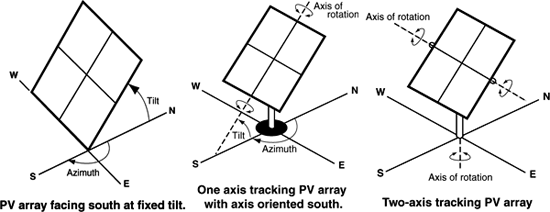
\includegraphics{pvwatts_tracking.png}

\paragraph{Field: System Losses}\label{field-system-losses}

Fraction of the system output lost due to losses in a real system that
are not explicitly calculated by the PVWatts model equations.

Default: 0.14.

\paragraph{Field: Array Geometry
Type}\label{field-array-geometry-type}

One of:

\begin{itemize}
\tightlist
\item
  \texttt{TiltAzimuth} - The tilt and azimuth angles are specified in
  the next two fields. An unshaded array is assumed.
\item
  \texttt{Surface} - The array geometry (tilt and azimuth) as well as
  shading is determined from surface referenced.
\end{itemize}

\paragraph{Field: Tilt Angle}\label{field-tilt-angle}

The tilt angle is the angle from horizontal of the photovoltaic modules
in the array. For a fixed array, the tilt angle is the angle from
horizontal of the array where \SI{0}{\degree} = horizontal, and \SI{90}{\degree} = vertical. For
arrays with one-axis tracking, the tilt angle is the angle from
horizontal of the tracking axis. The tilt angle does not apply to arrays
with two-axis tracking.

Default: \SI{20}{\degree}

\paragraph{Field: Azimuth Angle}\label{field-azimuth-angle}

For a fixed array, the azimuth angle is the angle clockwise from true
north describing the direction that the array faces. An azimuth angle of
\SI{180}{\degree} is for a south-facing array, and an azimuth angle of \SI{0}{\degree}
is for a north-facing array.

For an array with one-axis tracking, the azimuth angle is the angle
clockwise from true north of the axis of rotation. The azimuth angle
does not apply to arrays with two-axis tracking.

Default: \SI{180}{\degree}

\paragraph{Field: Surface Name}\label{generatorpvwatts-field-surface-name}

This is the name of a surface that defines the location and geometry of
the array. Required if Array Geometry Type is \texttt{Surface}. Shading
will be calculated for this surface regardless of whether the array has
1- or 2-axis tracking.

\paragraph{Field: Ground Coverage
Ratio}\label{field-ground-coverage-ratio}

The ground coverage ratio (GCR) applies only to arrays with one-axis
tracking, and is the ratio of module surface area to the area of the
ground or roof occupied by the array. A GCR of 0.5 means that when the
modules are horizontal, half of the surface below the array is occupied
by the array. An array with wider spacing between rows of modules has a
lower GCR than one with narrower spacing. A GCR of 1 would be for an
array with no space between modules, and a GCR of 0 for infinite spacing
between rows. Typical values range from 0.3 to 0.6.

Default: 0.4

\subsubsection{Outputs Description}\label{outputs-description}

\begin{itemize}
\item
  HVAC,Average,Generator Produced DC Electricity Rate {[}W{]}
\item
  HVAC,Sum,Generator Produced DC Electricity Energy {[}J{]}
\item
  HVAC,Average,Plane of Array Irradiance $\left [\frac{\text{W}}{\text{m}^2} \right ]$
\item
  HVAC,Average,Generator PV Cell Temperature {[}C{]}
\end{itemize}


\subsection{Generator:WindTurbine}\label{generatorwindturbine}

A wind turbine is a component that converts the kinetic energy of the surrounding airstream into electricity. This model is intended to calculate the electrical power that a wind turbine system produces. The performance of wind turbine systems is dependent on the local environmental conditions such as wind speed and density of air at the height of the systems. An analysis of these conditions is necessary to accurately estimate power output. The model obtains the weather information from the weather data file in EnergyPlus and then determines the wind speed and air density at the specific height of the system. It also requires the user to input the annual average wind speed measured at the local site and the height of the measurement so that it factors in differences between the weather file wind data and the local wind data.

The model employs the general kinetic energy equation to calculate the performance characteristics of the horizontal axis wind turbine (HAWT) systems. It provides a simple approximation algorithm when the power coefficient, Cp, is available which represents the efficiency of the wind turbine in the wind power extraction from the ambient air stream. It also allows the user to input experimental constants so that the power coefficient can precisely be determined according to the characteristic of the airfoil of the system. As for the vertical axis wind turbine (VAWT) systems, it employs the general mathematical equations for straight-bladed Darrieus-type VAWT systems, which are common to VAWT systems. Various types of VAWT systems such as the Savonius-type and the curved-blade (or Egg-beater) type may be simulated with this same model.

It includes two different types of dynamic power control: FixedSpeedFixedPitch (FSFP) and VariableSpeedFixedPitch (VSFP). Currently, it does not include an algorithm for modeling pitch control such as FixedSpeedVariablePitch (FSVP) and VariableSpeedVariablePitch (VSVP). If the control type of the wind turbine is either FSVP or VSVP, the control type of VSFP will be assumed. In addition, constant power generation is assumed when the ambient wind speed is between the rated wind speed and the cut out wind speed, if the user specifies one of the last three options. The model also has the ability to account for transient losses associate with the power produced during dynamic control by a user-specified fraction.

The model does not include detailed algorithms for generators and inverters due to concerns for computational convergence, time, and usability. Instead, all conversion losses of these subsystems are included by applying a user-supplied total system efficiency to the maximum power extraction of the wind turbine. The field of the total system efficiency must be specified by the user.

\subsubsection{Inputs}\label{inputs-23}

\paragraph{Field: Name}\label{field-name-27}

A unique user assigned name for a particular wind turbine system. Any reference to this unit by another object will use this name.

\paragraph{Field: Availability Schedule Name}\label{field-availability-schedule-name-8-000}

The name of the schedule (ref: Schedule) that denotes whether the wind turbine system can run during a given time period. A schedule value greater than 0 (usually 1 is used) indicates that the unit can be on during the time period. A value less than or equal to 0 (usually 0 is used) denotes that the unit is off and will not operate for the time period. If this field is blank, the schedule has values of 1 for all time periods.

\paragraph{Field: Rotor Type}\label{field-rotor-type}

This field is the type of axis of the wind turbine. The user specifies either a horizontal axis wind turbine or a vertical axis wind turbine. Each type of wind turbine employs a different algorithm for the calculation of the electrical power output of the wind turbine. The default value is HorizontalAxisWindTurbine.

\paragraph{Field: Power Control}\label{field-power-control}

This field is the type of rotor control for the wind turbine. This protects the system against the overloading for a system with no speed or pitch control and also to maximize the energy yield for the system. Four different control types are classified in the literature: FixedSpeedFixedPitch (FSFP), FixedSpeedVariablePitch (FSVP), VariableSpeedFixedPitch (VSFP), and VariableSpeedVariablePitch (VSVP). Currently, FSFP and VSFP types can be modeled in EnergyPlus. The other two types will be modeled as VSFP. If the first FSFP control type is chosen, the model assumes the maximum power at a fixed rotor speed when the power output predicted is greater than the maximum until the rotor speed reaches the maximum wind speed (see next field). If one of the last three control options is chosen, the model assumes that the system produces a constant power at the rated wind speed when the wind speed is between the rated wind speed and cut-out wind speed. The default value is VariableSpeedFixedPitch (VSFP).

\paragraph{Field: Rated Rotor Speed}\label{field-rated-rotor-speed}

This field is the maximum rotational speed of the rotor at the rated power of the wind turbine in rev/min (revolution per minute). It is used to determine the tip speed ratio of the rotor and relative flow velocity incident on a single blade of the VAWT systems.

\paragraph{Field: Rotor Diameter}\label{field-rotor-diameter}

This field is the diameter of the rotor in meters. Note that this field is not the height of the blade, but the diameter of the perpendicular circle from the vertical pole in the VAWT systems. It determines the swept area of the rotor of the HAWT systems and the chordal velocity of the VAWT systems.

\paragraph{Field: Overall Height}\label{field-overall-height}

This field is the height of the hub of the HAWT system, or of the pole of the VAWT system in meters. It is necessary to estimate local air density and the wind speed at this particular height where the wind turbine system is installed.

\paragraph{Field: Number of Blades}\label{field-number-of-blades}

This field is the number of blades of the wind turbine. The azimuth angle of the rotor of the VAWT system is determined by dividing 360 degree by this field so that the model determines the chordal velocity component and the normal velocity component of the system. The default value is 3.

\paragraph{Field: Rated Power}\label{field-rated-power}

This field is the nominal power output of the wind turbine system at the rated wind speed in Watts. Note that the user should input the maximum power of the system with no control, i.e., FSFP control type, can physically produce. Manufacturers data also indicates it as peak power or rated capacity . If the local wind speed is greater than the rated wind speed, the model assumes constant power output of this field.

\paragraph{Field: Rated Wind Speed}\label{field-rated-wind-speed}

This field is the wind speed that the wind turbine system indicates the peak in the power curve in m/s. The system produces the maximum power at this speed and the speed of the rotor is managed based on this wind speed.

\paragraph{Field: Cut In Wind Speed}\label{field-cut-in-wind-speed}

This field is the lowest wind speed where the wind turbine system can be operated in m/s. No power generation is achieved as long as the ambient wind speed is lower than this speed.

\paragraph{Field: Cut Out Wind Speed}\label{field-cut-out-wind-speed}

This field is the greatest wind speed in m/s. When the wind speed exceeds this value, the wind turbine system needs to be stopped because of inefficiencies in the system. All systems that have either pitch or speed control must be stopped when the ambient wind speed exceeds this speed. Note that the user should input a wind speed above which physical damage to the system might be caused in the case of a FSFP system. It appears as extreme/survival/design wind speed in the literature. The system will be turned off when the ambient wind speed is over this speed.

\paragraph{Field: Fraction System Efficiency}\label{field-fraction-system-efficiency}

This field is the overall system efficiency of the wind turbine system. It includes all the conversion losses as well as transient losses during the dynamic control when the ambient wind speed is between the rated wind speed and cut-out wind speed (see previous fields). The user also has the ability to specify delivery losses from the system to the local area. If the user does not enter a fraction, the model assumes the default value of 0.835. Note that the fraction must be between zero and one.

\paragraph{Field: Maximum Tip Speed Ratio}\label{field-maximum-tip-speed-ratio}

This field is the maximum tip speed ratio between the rotor velocity and ambient wind velocity. The rotor speed varies with this ratio to maximize the power output when the rotor control types are variable speed ones. This field allows the user to adjust the power output from the particular system or to find the optimal tip speed ratio of the system. Optimal tip speed ratio is dependent on the number of blades. It is typically about 6, 5, and 3 for two-bladed, three-bladed, and four-bladed rotor, respectively. For the vertical axis wind turbine, it is smaller than horizontal axis wind turbine, and varies with the chord area. The default and maximum values are 5.0 and 12.0.

\paragraph{Field: Maximum Power Coefficient}\label{field-maximum-power-coefficient}

This field is the maximum fraction of power extraction from ambient wind. If the user inputs this field, the simple approximation model is assumed. The model simply employs the value of this field into the general kinetic energy equation, so that the power output is obtained. The user can obtain this field with a simple calculation from the power curve published in almost all manufacturers' specifications by using the kinetic energy equation as:

\begin{equation}
{C_p} = \frac{P}{{0.5\rho A{V^3}}}
\end{equation}

where

\emph{P} = power production at the rated wind speed {[}W{]}

\emph{ρ} = density of air {[}kg/m3{]}

\emph{A} = swept area of rotor {[}m2{]}

\emph{V} = rated wind speed {[}m/s{]}

\emph{C\(_{p}\)} = power coefficient

The maximum and default values are 0.59 and 0.35.

\paragraph{Field: Annual Local Average Wind Speed}\label{field-annual-local-average-wind-speed}

This field is the local annual average wind speed that represents a representative wind profile at the location of the system in m/s. It is used to factor the difference in wind speed between the weather file wind data and the locally measured wind data so that the model minimizes uncertainties caused by improper wind data at the particular location. Considerable differences between the weather file wind data and the local wind data typically appear. The user thus needs to enter this field in order to obtain accurate local wind data. The model internally determines a multiplier and it is multiplied by the weather file wind data adjusted at the height of the system. If this field is not entered, then the model will use the wind speed from the design day or weather file information with only adjustment at the height of the rotor.

\paragraph{Field: Height for Local Average Wind Speed}\label{field-height-for-local-average-wind-speed}

This field is the height that the local wind speed is measured in meters. The annual average wind speed (see previous field) input by the user is internally recalculated by existing EnergyPlus functions at the height of the local station. This modified wind speed is then factored and applied to the weather file wind data. If the annual local average wind speed is not entered, this field is then assumed as zero. The minimum and default values are zero and 50 meters.

\paragraph{Field: Blade Chord Area}\label{field-blade-chord-area}

This field is the blade chord area of a single blade of VAWT system in m2. It is necessary to determine the net tangential and normal forces of a single blade.

\paragraph{Field: Blade Drag Coefficient}\label{field-blade-drag-coefficient}

This field is the blade drag coefficient for a specific blade. It is for determining the tangential and normal force coefficients with the blade lift coefficient (see next field) so that the model can calculate the power output from the system. The user should be able to obtain this parameter for a specific blade from the manufacturers data. This field is only valid for VAWT systems.

\paragraph{Field: Blade Lift Coefficient}\label{field-blade-lift-coefficient}

This field is the blade lift coefficient for a specific blade. It is for determining the tangential and normal force coefficients with the blade drag coefficient (see previous field) so that the model can calculate the power output from the system. The user should also be able to obtain it for a specific blade from the manufacturers data. This field is only valid for VAWT systems.

\paragraph{Field: Power Coefficient Parameter \textless{}x\textgreater{}}\label{field-power-coefficient-parameter-x}

These six fields are the parameters for the power coefficient equation shown below. These fields are used to determine the power coefficient of the system. The analytical approximation model of the power coefficient in EnergyPlus is:

\begin{equation}
{C_p} = {C_1}(\frac{{{C_2}}}{{{\lambda_i}}} - {C_3}\theta  - {C_4}{\theta ^x} - {C_5}){e^{ - \frac{{{C_6}(\lambda ,\theta )}}{{{\lambda_i}}}}}
\end{equation}

with

\begin{equation}
\frac{1}{{{\lambda_i}}} = \frac{1}{{\lambda  + 0.08\theta }} - \frac{{0.035}}{{{\theta ^3} + 1}}
\end{equation}

where

\(C_p\) = power coefficient

\(C_{1-6}\) = empirical power coefficient parameters

\(\lambda\) = tip speed ratio (often known as TSR)

\(\lambda_i\) = tip speed ratio at ith time step

\(\theta\) = azimuth angle of the pitch, 0 {[}degree{]}

If the user does not input any field of these parameters, the simple approximation model for the power coefficient will be used (see previous maximum power coefficient field). That is, the analytical approximation model of the power coefficient will be chosen only if the user inputs all these six parameters. The user also has the ability to modify each parameter when the specific value of the system is available. The default values are given in the table below.

\begin{longtable}[c]{@{}llllll@{}}
\toprule
C & C & C & C & C & C \tabularnewline
\midrule
\endfirsthead

\toprule
C & C & C & C & C & C \tabularnewline
\midrule
\endhead

0.5176 & 116 & 0.4 & 0.0 & 5.0 & 21 \tabularnewline
\bottomrule
\end{longtable}

These fields are only valid for HAWT systems.

An example input for the wind turbine is shown in below.

\begin{lstlisting}

Generator:WindTurbine,
  WT1,                     ! Name
  WT Schedule,     ! Availability Schedule Name
  HorizontalAxisWindTurbine,     ! Rotor type
  FixedSpeedVariablePitch,         ! Power control type
  41,                       ! Maximum rotational speed of the rotor {rev/min}
  19.2,                   ! Diameter of the rotor {m}
  30.5,                   ! Overall height of the system {m}
  3,                         ! Number of blades
  55000,                 ! Rated power output at the rated wind speed {W}
  11,                       ! Rated wind speed {m/s}
  3.5,                     ! Cut In wind speed {m/s}
  25,                       ! Cut Out wind speed {m/s}
  0.835,                 ! Overall wind turbine system efficiency
  8,                         ! Maximum tip speed ratio
  0.4,                     ! Maximum power coefficient
  6.4,                     ! Annual local wind speed {m/s}
  50,                       ! Height of local meteorological station {m}
  ,                           ! Blade chord area {m2}
  ,                           ! Blade drag coefficient
  ,                           ! Blade lift coefficient
  0.5176,               ! Power Coefficient C1
  116,                     ! Power Coefficient C2
  0.4,                     ! Power Coefficient C3
  0,                         ! Power Coefficient C4
  5,                         ! Power Coefficient C5
  21;                       ! Power Coefficient C6
\end{lstlisting}

\subsubsection{Outputs}\label{outputs-12-001}

\begin{itemize}
\item
  HVAC,Average, Generator Produced Electricity Rate {[}W{]}
\item
  HVAC,Sum, Generator Produced Electricity Energy {[}J{]}
\item
  HVAC,Average, Generator Turbine Local Wind Speed {[}m/s{]}
\item
  HVAC,Average, Generator Turbine Local Air Density {[}kg/m3{]}
\item
  HVAC,Average, Generator Turbine Power Coefficient {[]}
\item
  HVAC,Average, Generator Turbine Tip Speed Ratio {[]}
\item
  HVAC,Average, Generator Turbine Chordal Component Velocity {[}m/s{]}
\item
  HVAC,Average, Generator Turbine Normal Component Velocity {[}m/s{]}
\item
  HVAC,Average, Generator Turbine Relative Flow Velocity {[}m/s{]}
\item
  HVAC,Average, Generator Turbine Attack Angle {[}deg{]}
\end{itemize}

\paragraph{Generator Produced Electricity Rate {[}W{]}}\label{generator-produced-electric-power-w-4}

This report is the electric power that the wind turbine system produces.

\paragraph{Generator Produced Electricity Energy {[}J{]}}\label{generator-produced-electric-energy-j-4}

This report is the electric energy that the wind turbine system produces.

\paragraph{Generator Turbine Local Wind Speed {[}m/s{]}}\label{generator-turbine-local-wind-speed-ms}

This report is the local wind speed at the specific height of the wind turbine.

\paragraph{Generator Turbine Local Air Density {[}kg/m3{]}}\label{generator-turbine-local-air-density-kgm3}

This report is the local density of the air at the specific height of the wind turbine.

\paragraph{Generator Turbine Tip Speed Ratio {[]}}\label{generator-turbine-tip-speed-ratio}

This report is the ratio between the rotational speed of the tip of the blades and the ambient wind speed at the height of the hub or pole of the wind turbine.

\paragraph{Generator Turbine Power Coefficient {[]}}\label{generator-turbine-power-coefficient}

This report represents the efficiency of the power extraction from the ambient wind of the wind turbine. It is function of the tip speed ratio and pitch angle. It is only valid for HAWT systems.

\paragraph{Generator Turbine Chordal Component Velocity {[}m/s{]}}\label{generator-turbine-chordal-component-velocity-ms}

This report is the axial velocity component along the chord of the wind turbine system. It is only valid for VAWT systems.

\paragraph{Generator Turbine Normal Component Velocity {[}m/s{]}}\label{generator-turbine-normal-component-velocity-ms}

This report is the axial velocity component of the rotor of the wind turbine system. It is only valid for VAWT systems.

\paragraph{Generator Turbine Relative Flow Velocity {[}m/s{]}}\label{generator-turbine-relative-flow-velocity-ms}

This report is the local relative flow velocity that represents actual direction and velocity incident on the blades. It is the square root of the sum of both chordal velocity component and normal velocity component. It is only valid for VAWT systems.

\paragraph{Generator Turbine Attack Angle {[}deg{]}}\label{generator-turbine-attack-angle-deg}

This report is the azimuth angle between the relative flow velocity and the plane of chord. It varies as the wind speed increases, so that the lift and drag forces change.

\begin{center}\rule{0.5\linewidth}{0.4pt}\end{center}

\protect\hyperlink{ux5fftnref1}{{[}1{]}} Ulleberg Ø . (1997) Simulation of autonomous PV-H2 systems: analysis of the PHOEBUS plant design, operation and energy management. In \emph{Proceedings of ISES 1997 Solar World Congress}, August 24-30, Taejon, Korea.

Ulleberg Ø . (1998) \emph{Stand-Alone Power Systems for the Future: Optimal Design, Operation \& Control of Solar-Hydrogen Energy Systems}. PhD thesis, Norwegian University of Science and Technology, Trondheim.
